\documentclass[12pt, a4paper,oneside]{book}
% Подключение библиотеки
\usepackage{/Users/vladbelousov/Desktop/Semestr_4-FP-NSU/Настройка/library}

\begin{document}

\begin{titlepage}
    \thispagestyle{empty}  % Отключаем нумерацию страницы на титульном листе
    \centering
    \vspace*{1cm}  % Отступ сверху

    \textbf{\huge Конспект лекций по дисциплине}  \\[1.5cm]  % Название
    \textbf{\huge Электродинамика и оптика }  \\[2cm]   % Название дисциплины (оставьте пустым для добавления вручную)
    \textbf{\Large Новосибирский государственный университет} \\[0.5cm]
    \textbf{\large Физический факультет} \\[0.5cm]
    \textbf{\large 4-й семестр} \\[0.5cm]
    \textbf{\large 2025 год} \\[10cm]

    \begin{flushright}
        \large Студент: Б.В.О \\[0.5cm]  % Ваше имя
        Преподаватель: Синицкий Станислав Леонидович  % Ф.И.О. преподавателя
    \end{flushright}
\end{titlepage}

\tableofcontents  % Создание оглавления

\def\mainfile{}  % Определяем макрос для основного файла
%Февраль
% Условная компиляция для самостоятельной работы
\ifdefined\mainfile
    % Если это часть основного файла, не добавляем начало и конец документа
\else
    \documentclass[12pt, a4paper]{report}
    \usepackage{/Users/vladbelousov/Desktop/Semestr_4-FP-NSU/Настройка/library}
    \usepackage[utf8]{inputenc} % Подключение поддержки UTF-8
    \begin{document}
\fi

%%-------------------------------%%

\chapter{Электромагнитные волны.}

\section{Свободное электромагнитное поле. Волновое уравнение.  }

\begin{definition}[Свободное]   
означает без токов и зарядов \( \Rightarrow \rho =0 , \vec{j}= 0   \) 
\end{definition}

\[ 
\begin{aligned}
    \begin{cases}
         \displaystyle \mathrm{rot} \vec{ E} =-\frac{1}{c}\frac{\partial\vec{B}}{\partial t}, \quad \mathrm{div} \vec{B}=0 \\
        \displaystyle \mathrm{rot} \vec{H} =\frac{1}{c}\frac{\partial\vec{D}}{\partial t}, \quad \mathrm{div} \vec{D}=0     
    \end{cases} 
    + \text{Грани. условия} 
    \text{ } 
    \begin{cases}
        (B_n)| = 0 \quad (E_{\tau} )= 0 \\ 
        (D_n)| = 0 \quad (H_{\tau} )= 0 
    \end{cases}
\end{aligned}
 \] 

 \textit{Два типа векторных полей:} 

 1. Вихревые: \( \mathrm{div}\vec{F}= 0    \)  (нет источников истоков этого поля \( \Rightarrow  \) силовые линии либо замкнуты, либо уходят на бесконечность)

\begin{center}
    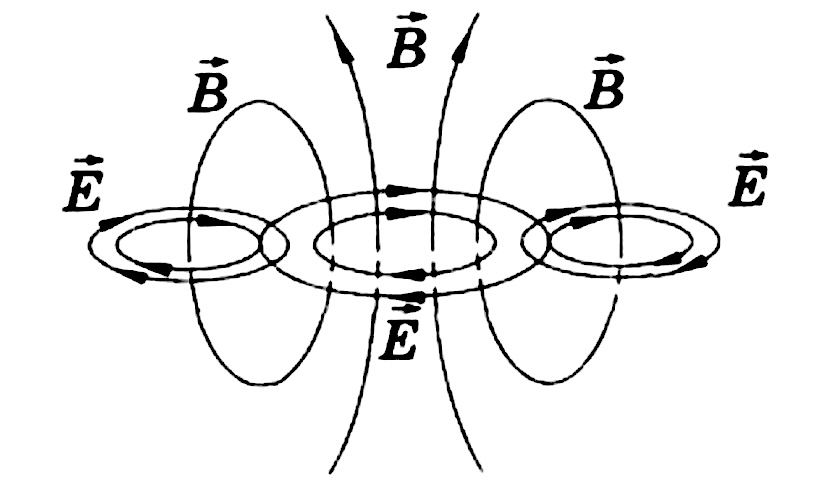
\includegraphics[width=0.3\textwidth]{/Users/vladbelousov/Desktop/Semestr_4-FP-NSU/ЭиО/Лекции_по_дням/image/1.jpeg}
\end{center}

 2. Потенциальные: \( \mathrm{rot} \vec{F} =0 \). Силовые линии выходят или входят в области стоков и истоков (где \( \mathrm{div} \vec{F} \neq 0     \)) или на бесконечности. 

\begin{center}
    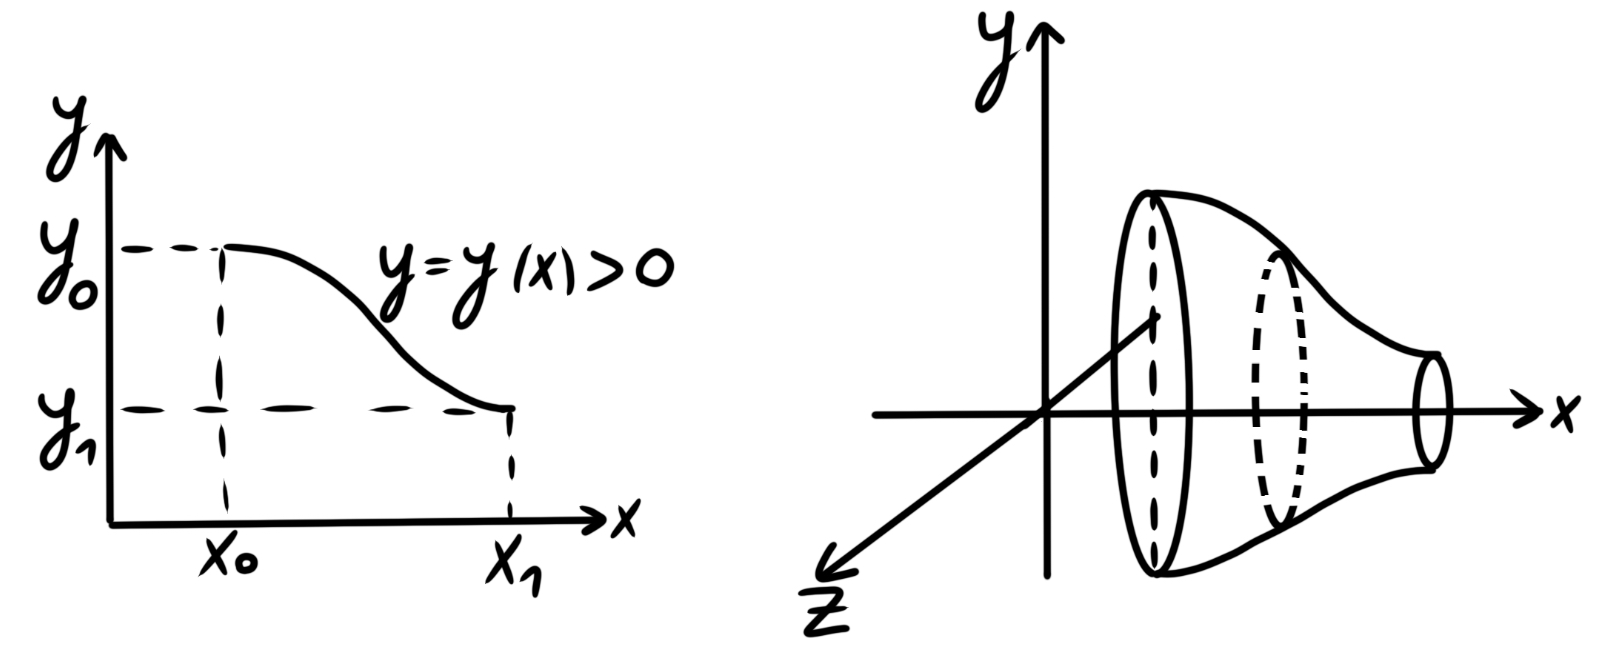
\includegraphics[width=0.5\textwidth]{/Users/vladbelousov/Desktop/Semestr_4-FP-NSU/ЭиО/Лекции_по_дням/image/2.png}
\end{center}

Далее мы будем рассматривать только вихревые поля (т.е. \( \mathrm{div} \vec{B} = 0 ,\mathrm{div} \vec{D} = 0  \))

Неизвестные 3 компоненты каждого поля: \( \vec{E},\vec{D},\vec{B},\vec{H}\) - 12 неизвестные функций. Мы можем решить эту систему при помощи уравнений Максвелла \( + \)  материальные уравнения: \( \vec{B}=\vec{B}(H), \vec{E}=\vec{E}(D) \).

Простая модель среды: \( \vec{B}=\mu\vec{H}, \vec{D}=\varepsilon \vec{E} \), где \( \mu = \mathrm{const}  , \varepsilon =\mathrm{const}   \), годится для вакуума (\(\mu=1, \varepsilon=1  \)) и для многих других сред/материалов при низких значения полей \( \vec{E}, \vec{B} \)  и при невысоких частотах \( f < 10^8 \) Гц. 
 
\newpage

\textit{Волновое уравнение:} 

Рассмотрим \(  \displaystyle  \mathrm{rot} (\mathrm{rot} \vec{E}  )= -\frac{\mu}{c}  \frac{\partial}{\partial t} \mathrm{rot } \vec{H}= - \frac{\mu \varepsilon}{ c ^2} \frac{\partial ^2}{\partial t ^2}     \vec{E} \\ \) 

Распишем чему равен \( \mathrm{rot}(\mathrm{rot}\vec{E}  )   \) :

\[         \displaystyle \mathrm{rot} (\mathrm{rot} \vec{E}  )= \nabla \underbrace{\mathrm{div} \vec{E}}_{\frac{1}{\varepsilon} \mathrm{div}\vec{D}=0   }    - \Delta \vec{E}   \] 

Получаем нашу систему:

\[
\begin{aligned}
    \begin{cases}
        \displaystyle \Delta \vec{E}- \frac{\mu \varepsilon}{c ^2} \frac{\partial ^2 \vec{E}}{\partial t ^2} =0 \\
        \displaystyle \mathrm{div}   \vec{E}=0 
    \end{cases} 
    \quad \quad  (1)
\end{aligned} 
\] 

Так же делаем с \( \mathrm{rot }(\mathrm{rot}\vec{B})\) и получаем: 

\[
\begin{aligned}
    \begin{cases}
        \displaystyle  \Delta \vec{B} - \frac{\mu \varepsilon}{c ^2} \frac{\partial ^2 \vec{B}}{\partial t ^2} =0 \\
        \displaystyle \mathrm{div}   \vec{B}=0
    \end{cases}
    \quad \quad  (2)
\end{aligned} 
\]

Согласование решений (1) и (2): 

1) Решаем (1) и \( \vec{E} \)  подстваляем в уравнение Максвелла \( \to  \vec{B} \);

2) Решаем (2) и \( \vec{B} \)  подстваляем в уравнение Максвелла \( \to  \vec{E} \);

Различные простейшие решения волнового уравнения: 

1) Плоские волны: все ненулевые компоненты полей \( \vec{ E} ,\vec{ B} \) завися от одной координаты (например от z)  и времени t; 

\begin{center}
    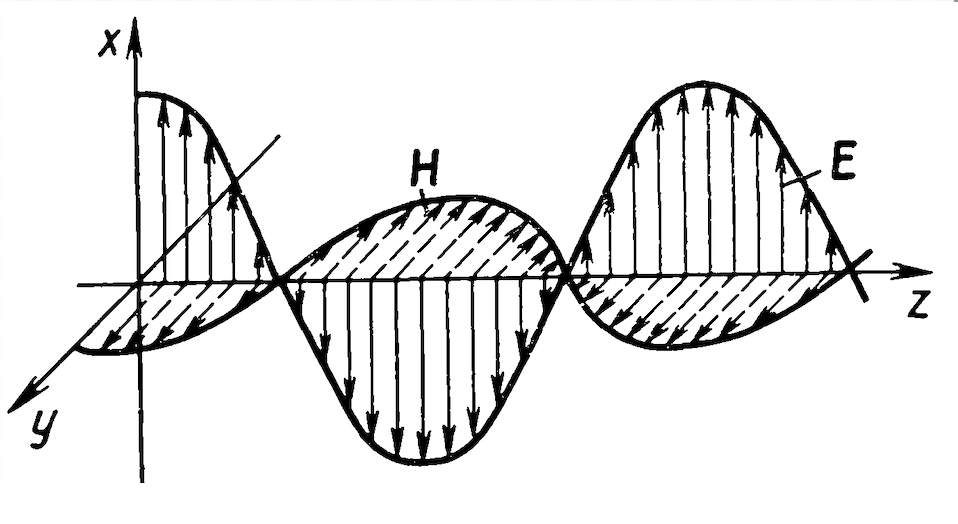
\includegraphics[width=0.3\textwidth]{/Users/vladbelousov/Desktop/Semestr_4-FP-NSU/ЭиО/Лекции_по_дням/image/3.png}
\end{center}


2) Цилиндрические волны: все ненулевые компоненты полей \( \vec{ E} ,\vec{ B} \) зависят от \( \vec{ r}  \)  - расстояния от точки наблюдения до некоторой оси (центра волны) и от времени t; 

3) Сферическая волна: все ненулевые компоненты полей \( \vec{ E} ,\vec{ B} \) зависят от \( \vec{r}  \)  - расстояния от точки наблюдения до центра волны.

\begin{center}
    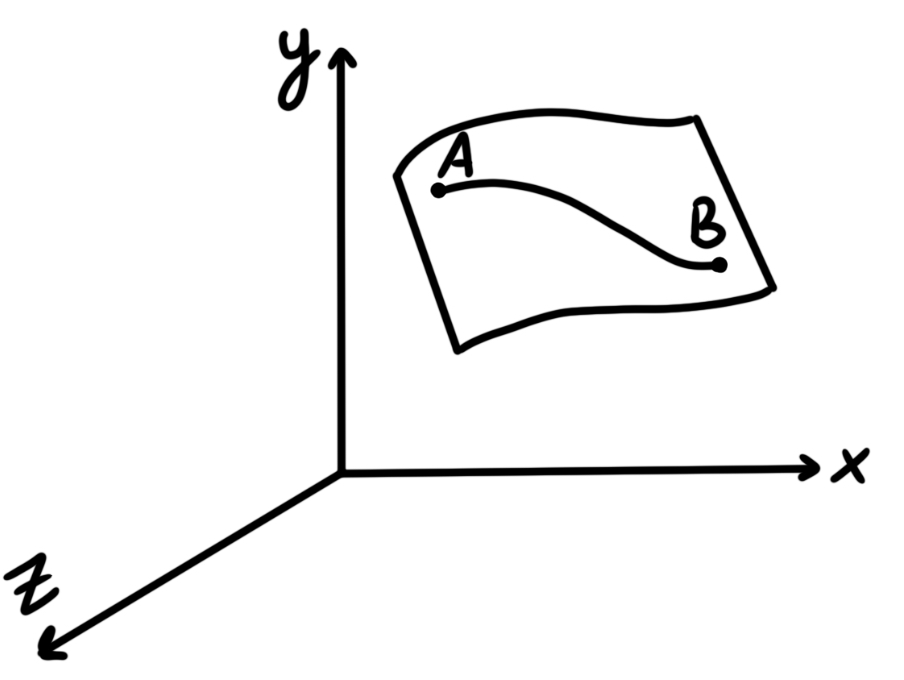
\includegraphics[width=0.3\textwidth]{/Users/vladbelousov/Desktop/Semestr_4-FP-NSU/ЭиО/Лекции_по_дням/image/4.png}
\end{center}

\newpage

\section{Плоские волны. }

\[ \frac{\partial ^2 }{\partial t^2 } \vec{E} - \frac{\mu \varepsilon}{c ^2} \frac{\partial ^2 \vec{ E}}{\partial t ^2 } =0 \text{ , для примера }  E_x : \left( \frac{\partial}{\partial z} - \frac{\sqrt{\mu \varepsilon} }{c} \frac{\partial}{\partial t }   \right) \left( \frac{\partial}{\partial z} + \frac{\sqrt{\mu \varepsilon} }{c} \frac{\partial}{\partial t } \right) E_x = 0  \quad  (*)  \] 

Под f подразумевается \( E_x  \) или \( E_y \)  

\begin{gather*}
    \xi = z - \frac{c t}{ \sqrt{\mu \varepsilon} }, \quad \eta = z + \frac{c t}{ \sqrt{\mu \varepsilon} } \quad ( \text{замена переменных} )  \\
    \frac{\partial}{\partial z } f ( \xi ( z,t), \eta(z,t) ) = \frac{\partial f}{\partial \xi }  \underbrace{\frac{\partial \xi }{\partial z }}_{=1} + \frac{\partial f }{\partial \eta  }   \underbrace{\frac{\partial \eta }{\partial z }}_{=1}= \frac{\partial f}{\partial \xi } + \frac{\partial f}{ \partial \eta } \\
    \frac{\sqrt{\mu \varepsilon}}{c}  \frac{\partial f }{\partial t}      = \frac{\sqrt{\mu \varepsilon}}{c} \left( \frac{\partial f }{\partial \xi } \left( - \frac{c}{\sqrt{\mu \varepsilon}}\right) + \frac{\partial f}{\partial \eta } \left( \frac{c}{\sqrt{\mu \varepsilon}}  \right)  \right)=- \frac{\partial f}{\partial \xi } + \frac{\partial f}{ \partial \eta }  \\ 
    \frac{\partial}{\partial z } \to  \frac{\partial}{\partial \xi } + \frac{\partial}{\partial \eta }, \quad \frac{\sqrt{\mu \varepsilon}}{c}\frac{\partial}{\partial t} \to \frac{\partial}{\partial \eta }- \frac{\partial }{\partial \xi } \\
\end{gather*} 
Подставляем в (*):

\[     \left( \frac{\partial }{\partial \xi  }+ \cancel{\frac{\partial}{\partial \eta }}  - \cancel{\frac{\partial}{\partial \eta }}  + \frac{\partial}{\partial \xi  }     \right) \left( \cancel{\frac{\partial}{\partial \xi }}  +\frac{\partial}{\partial \eta } +\frac{\partial}{\partial \eta } - \cancel{\frac{\partial}{\partial \xi }}  \right) E_x ( \varepsilon,\mu)= 0 \Rightarrow  4 \cdot \frac{\partial}{ \partial\mu \partial\varepsilon}E_x ( \varepsilon,\mu)= 0  \] 

Так как смешанные производные коммутируют ( \(\displaystyle  \frac{\partial}{\partial \mu \partial \varepsilon}= \frac{\partial}{\partial \varepsilon \partial \mu}   \)) и уравнение равно нулю, то \( \vec{E_x} \) можно представить в виде суммы двух функций.

\[     E_x (z,t) = f \left(z- \frac{c}{\sqrt{ \mu \varepsilon }}   \right)+ g \left(  z+ \frac{c}{\sqrt{ \mu \varepsilon }} \right) \\ 
\] 

Так же решения являются произвольные функции от своих аргументов: \( f(\xi) , f(\eta) \). В этом убеждают значения соответствующих вторых производных:

\[ \frac{\partial ^2 f(\xi \backslash \eta )}{ \partial z ^2} = \frac{ d ^2 f(\xi \backslash \eta )}{d (\xi \backslash \eta ) ^2}, \text{ } \frac{\partial ^2 f(\xi \backslash \eta ) }{ \partial t ^2} = \left( \pm \frac{c}{\sqrt{\mu \varepsilon}}  \right) ^2\frac{ d ^2 f(\xi \backslash \eta)}{d (\xi \backslash \eta)  ^2}   \] 

Физически это отражает принцип суперпозиции волн: любое решение может быть представлено в виде комбинации волн, движущихся в противоположных направлениях.

По аналогии можем записать \( \vec{E_y} \) :

\[ \displaystyle     E_y (z,t) = p \left(z- \frac{c}{\sqrt{ \mu \varepsilon }}   \right)+ h \left(  z+ \frac{c}{\sqrt{ \mu \varepsilon }} \right) \\ 
, \text{ где } \forall p,h  \] 


Свойства плоских волн: 

1) Из определения, что плоские волны поперечные, то-есть перпендикулярны к направлению своего движения: \( E_z = 0 , B_z =0  \).

\begin{proof}
    \[ \displaystyle  \mathrm{div}\vec{D}=\varepsilon \mathrm{div}\vec{E} =0 = \varepsilon \left( \underbrace{\frac{\partial E_x }{\partial x }}_{=0} + \underbrace{\frac{\partial E_y }{\partial y }}_{=0}+\frac{\partial E_z }{\partial z }  \right) \Rightarrow \frac{\partial \vec{E_z} }{\partial z }=0        \]

\begin{gather*}
    \mathrm{rot } \vec{H}= \frac{\varepsilon}{c} \frac{\partial \vec{E}}{\partial t} \Rightarrow \underbrace{\frac{\partial \vec{H_x}}{\partial x }}_{=0}  - \underbrace{\frac{\partial \vec{H_y}}{\partial y }}_{=0}   = \frac{\varepsilon}{c} \frac{\partial \vec{E_z} }{\partial t} \Rightarrow  \frac{\partial \vec{E_z} }{\partial t}=0
\end{gather*}

То есть все сводится к тому, что наше поле \( \vec{E_z} =E_0= \mathrm{const}\), но такое неизменное во времени однородное поле к волне отношения не имеет. Следовательно можно положить \( \vec{E_z}=0\), аналогично для \( \vec{B_z}=0 \).
\end{proof}



Пример: 

\begin{center}
    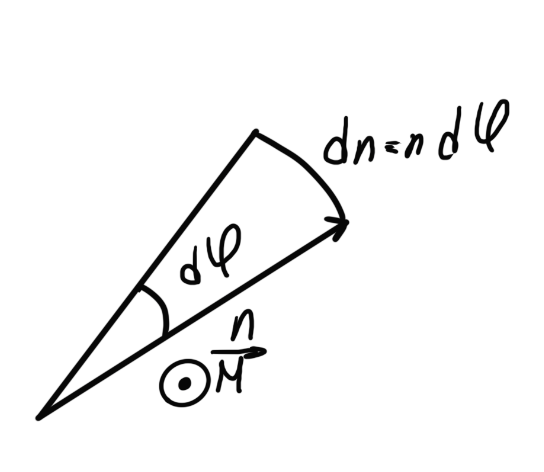
\includegraphics[width=0.7\textwidth]{/Users/vladbelousov/Desktop/Semestr_4-FP-NSU/ЭиО/Лекции_по_дням/image/5.png}
\end{center}

В максимуме \( \displaystyle z - \frac{c t}{ \sqrt{ \mu \varepsilon}} = 0   \) 

\[ \displaystyle \frac{\partial}{\partial t} \text{аргумент}=   \underbrace{\frac{dz}{dt} }_{V_{\Phi }  }- \frac{c}{\sqrt{ \mu \varepsilon}}=0   \] 

2) Связь поперечных полей в плоской волне: 

Рассмотрим бегущую волну в направлении оси z. В такой волне все величины являются функциями только от \(\displaystyle  \xi= z- \frac{c}{\sqrt{\mu \varepsilon } }t = z- ut   \) 

\[ \vec{E}= \vec{E}(\xi ) , \quad \vec{H}=\vec{H}(\xi ) \] 

Пусть \( \vec{E}= \vec{E}(\xi ) \)  произвольная функция, тогда  \(  H=H(\xi ) \) определяется из уравнения \( \displaystyle \mathrm{rot}\vec{E}= - \frac{\mu}{c} \frac{\partial \vec{H}}{\partial t}    \). Распишем левую и правую части уравнения:

\[ \mathrm{rot} \vec{E}(\xi )= \left[ \mathrm{grad} \xi \times  \frac{d \vec{E}}{d \xi }     \right]= [\vec{e_z}\times \frac{d \vec{E}}{d \xi }] = \frac{d}{d \xi  } [\vec{e_z}\times  \vec{E}(\xi )]   \] 

\[ \frac{\partial \vec{H}(\xi )}{\partial\xi }= \frac{d \vec{H}}{d\xi } \frac{\partial \xi }{\partial t}   = - u \frac{d \vec{H}}{d \xi } \] 

Подставляем это в уравнение:

\[ 
\frac{d}{d \xi} [\vec{e_z} \times \vec{E}(\xi)] = \frac{\mu}{c} u \frac{d \vec{H}}{d \xi} 
\]

Проинтегрировав по \( \xi \) получаем и подставив \( \displaystyle u=\frac{c}{\sqrt{\mu \varepsilon }} \) 


\[ \displaystyle  \sqrt{\varepsilon} \vec{E} = \sqrt{ \mu} [\vec{H}\times \vec{n}], \quad \sqrt{\mu} \vec{H} = \sqrt{ \varepsilon} [\vec{n}\times \vec{E}] \]

где \( \vec{n } \) - единичный вектор направления движения волны (\(  \vec{E} \perp \vec{B} \perp \vec{n} \)). 

3) \( \displaystyle \varepsilon E ^2 = \mu [ \displaystyle \vec{H}\times  \vec{n }] ^2 = \mu H ^2 n ^2 = \mu H ^2 | : 8 \pi \Rightarrow W_E = \frac{\varepsilon E ^2 }{8 \pi} =\frac{\mu B ^2 }{8 \pi} = W_B  \) 

4) \( \displaystyle \vec{S}= \frac{c}{4 \pi}   [ \vec{E}\times \vec{H }] \) - плотность потока энергии (вектор Умова-Пойтинга). 

\begin{gather*}
    \displaystyle \vec{S} = \frac{c}{4 \pi} [\vec{E } \times  \sqrt{\frac{\varepsilon}{\mu} }[\vec{n }\times  \vec{E}]]= \frac{c \varepsilon}{4 \pi \sqrt{ \mu \varepsilon}} \left( \vec{n}( \vec{E}\vec{E}) - \underbrace{\vec{E}( \vec{n }\vec{E})}_{=0}   \right)= \frac{c}{\sqrt{ \mu \varepsilon}} \vec{n} \left( \underbrace{\frac{\varepsilon E ^2 }{8 \pi}}_{W_E}  +\underbrace{\frac{\mu B ^2 }{8 \pi}  }_{W_B}  \right)   
\end{gather*}

\section{Плоские монохроматические волные (ПМВ).}

\( E_x, E_y, B_x, B_y \sim e^{-i \omega t}   \) 

\text{ }

\begin{minipage}{0.5\textwidth}
    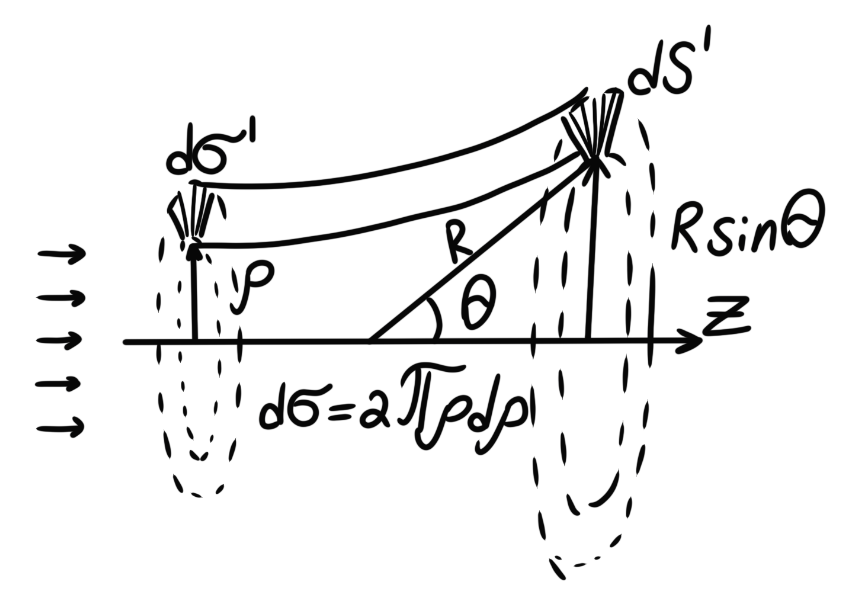
\includegraphics[width=0.5\textwidth]{/Users/vladbelousov/Desktop/Semestr_4-FP-NSU/ЭиО/Лекции_по_дням/image/6.png}
\end{minipage}
\begin{minipage}{0.5\textwidth}
    \text{В плоскости } \( z = z_0 , \vec{E}( z_0,t )= \vec{E_0}e^{-i \omega t} \Rightarrow  \) 
\end{minipage}

\begin{gather*}
    \displaystyle  \Rightarrow  \vec{E}( z,t)= \vec{E_0} e^{\frac{i \omega \sqrt{ \mu \varepsilon}}{c} \left( z- \frac{c}{\sqrt{\mu \varepsilon}} t -z_0  \right) }= \underbrace{\vec{E_0}e^{-\frac{i \omega \sqrt{ \mu \varepsilon}}{c}z_0} }_{\vec{E_{00}}} \cdot \underbrace{e^{\frac{i \omega \sqrt{ \mu \varepsilon}}{c} \left( z - \frac{c}{\sqrt{ \mu \varepsilon}}t  \right)} } _{f (z - \frac{c}{\sqrt{ \mu \varepsilon}}t)}   
\end{gather*}

\( \vec{E_0 } \perp \vec{n} = \vec{e_z} \Rightarrow \vec{E_0}=c_1 \vec{e_x}+ c_2 \vec{e_y}, c_1 \text{ и } c_2   \) - произвольные комплексные числа. 

\begin{definition}
    Волновое число \( k = \frac{\omega \sqrt{ \mu \varepsilon}}{c} = \frac{\omega}{V_{\text{волн.} } }   \) 
\end{definition}

\[ \displaystyle \vec{E}= \vec{E_{00}}e^{ikz- i \omega t } - \text{ для волны с } \vec{n} = \vec{e_z}, \qquad \vec{E}= \vec{E_{000}}e^{-ikz- i \omega t } - \text{ для волны с } \vec{n} = \vec{-e_z}  \] 

Универсальная запись полей ПМВ: 

\begin{center}
    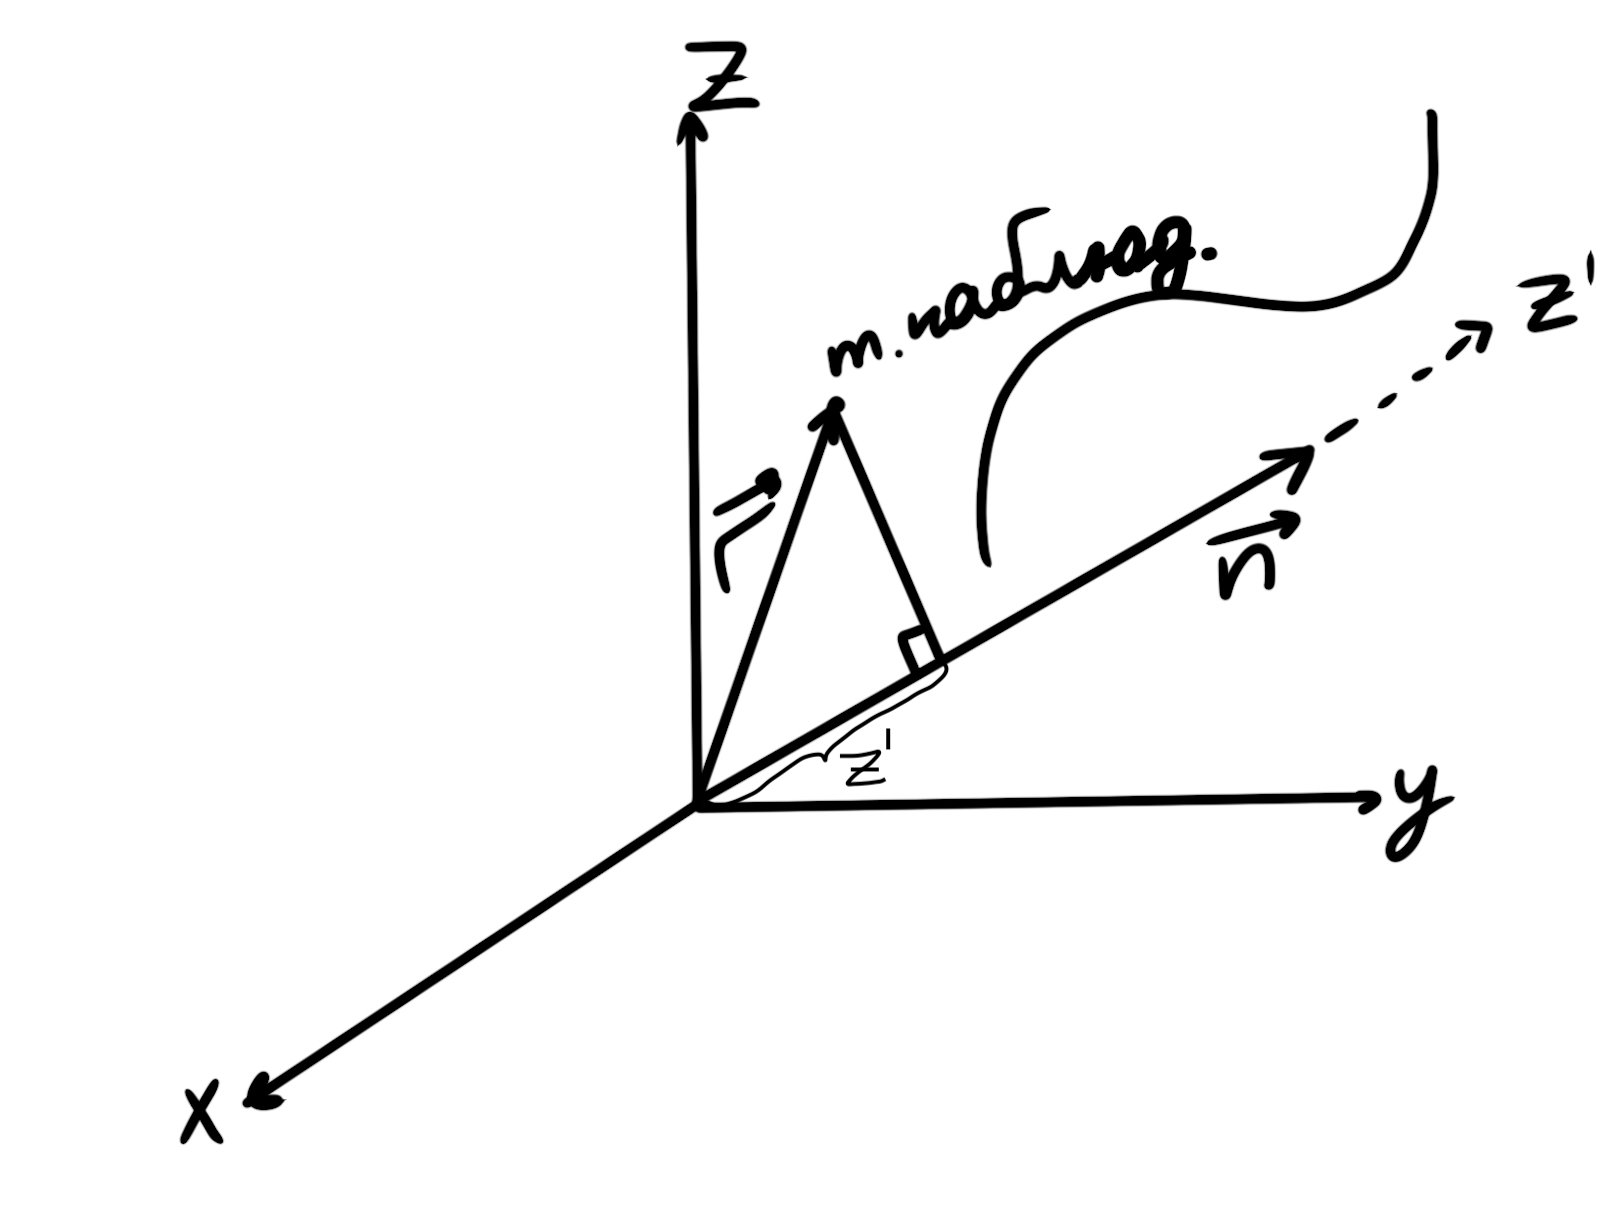
\includegraphics[width=0.3\textwidth]{/Users/vladbelousov/Desktop/Semestr_4-FP-NSU/ЭиО/Лекции_по_дням/image/7.png}
\end{center}

\[ \begin{aligned}
    \begin{cases}
        \displaystyle \vec{E}( z', t)= \vec{E_0 }e^{ikz' - i \omega t } \\  
        z'= (\vec{n}, \vec{r})
    \end{cases}
    \Rightarrow
    \displaystyle \vec{E}( z', t)= \vec{E_0}e^{ik(\vec{n}, \vec{r}) - i \omega t }= \vec{E_0}e^{i(\vec{k}, \vec{r}) - i \omega t }
\end{aligned} \] 
%%-------------------------------%%

% Закрытие документа, если файл компилируется отдельно
\ifdefined\mainfile
    % Если это основной файл, не нужно заканчивать документ
\else
    \end{document}
\fi
% Условная компиляция для самостоятельной работы
\ifdefined\mainfile
    % Если это часть основного файла, не добавляем начало и конец документа
\else
    \documentclass[12pt, a4paper]{report}
    \usepackage{/Users/vladbelousov/Desktop/Semestr_4-FP-NSU/Настройка/library}
    \usepackage[utf8]{inputenc} % Подключение поддержки UTF-8
    \begin{document}
\fi

%%-------------------------------%%

Свойство: ПМВ как и любая плоская волна имеет две степени свободы, то е сть обладает поляризацией.

Пример: ПМВ, бегущая по z, \( \vec{E}( z,t)= ( c_1 \vec{e_x}+ c_2 \vec{e_y} )e^{ikz- i \omega t}  (*) \), где \( c_1, c_2 \) - произвольные комплексные числа.

\begin{definition}
    Плоская волна, у которой вектор \( \vec{E} \) при \( \forall t \) во всем пространстве лежит в одной плоскости - плоскополяризованная (линейно поляризованная) волна.
\end{definition}

Выражение \( (*) \) - представляет собой сумму двух плоскополяризованных волн с поляризациями вдоль х и у. \( \forall  \)  плоскую волну можно разложить на две плоскополяризованные.

Рассмотрим несколько примеров. Пусть \( c_1= |c_1|e^{i \varphi} , c_2= |c_2|e^{ i \psi }  \) 

Реальное поле естть вещеестенная часть \( (*) \) 

\[ \mathrm{Re} ( \vec{E}(z,t))= |c_1|\vec{e_x}\cos (kz - \omega t + \varphi) + |c_2|\vec{e_y}\cos (kz - \omega t + \psi)   \] 

1) Пусть \( \psi = \varphi + 2 \pi m, m  \) - целое. 

\[ \Rightarrow \mathrm{Re}\vec{E }= |c_1|\vec{e_x}\cos (kz - \omega t + \varphi) + |c_2|\vec{e_y}\cos (kz - \omega t + \varphi + 2 \pi m)=   \]

\[= (|c_1| \vec{e_x} + |c_2\vec{e_y}) \cos (kz - \omega t + \varphi ) \quad  t = \mathrm{const}    \] 

\begin{center}
    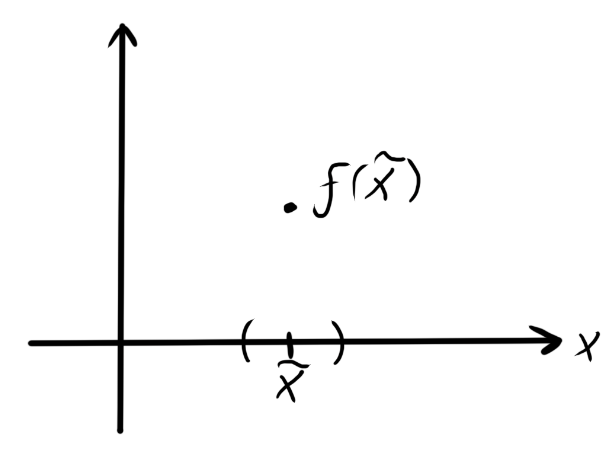
\includegraphics[width=0.5\textwidth]{/Users/vladbelousov/Desktop/Semestr_4-FP-NSU/ЭиО/Лекции_по_дням/image/8.png}
\end{center}

2) \(\displaystyle  \psi = \varphi +\frac{\pi}{2}    \) 

\[ \cos  ( kz - \omega t \varphi+ \frac{\pi}{2} )= \cos( kz - \omega t \varphi)\cos \frac{\pi}{2}-\sin( kz - \omega t \varphi)\sin  \frac{\pi}{2}   \] 

\[ \mathrm{Re}\vec{E }= |c_1|\vec{e_x}\cos ( kz - \omega t + \varphi)  - |c_2|\vec{e_y}\sin( kz - \omega t + \varphi)   \] 

3) \( \displaystyle \psi=\varphi - \frac{\pi}{2}  \) 

\[ \mathrm{Re}\vec{E }= |c_1|\vec{e_x}\cos ( kz - \omega t + \varphi)  + |c_2|\vec{e_y}\sin( kz - \omega t + \varphi)   \] 

\begin{center}
    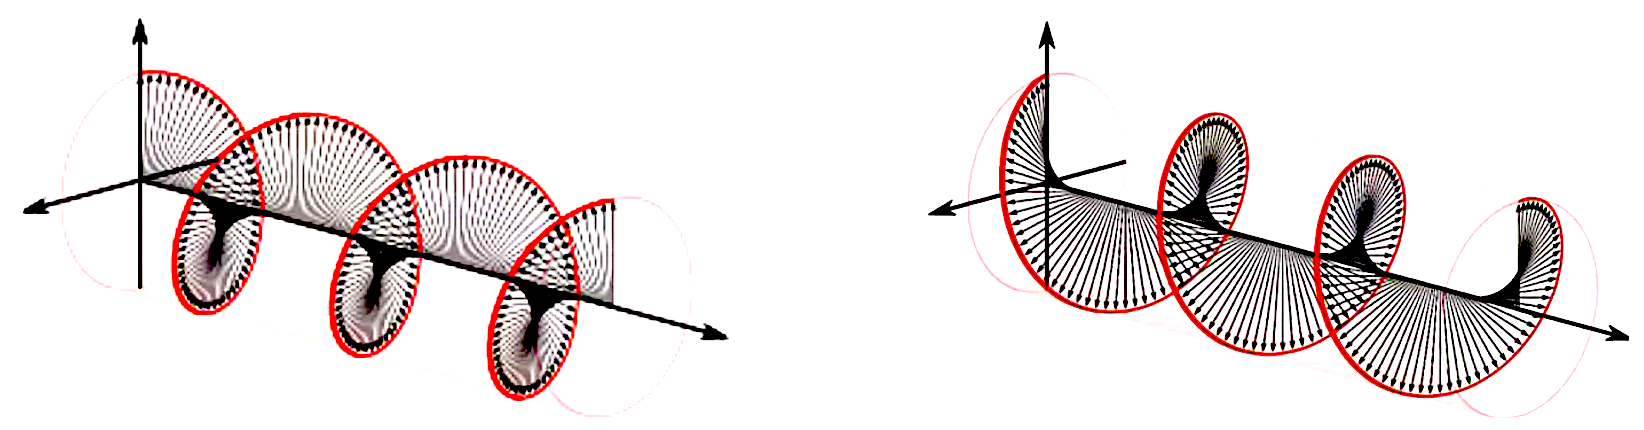
\includegraphics[width=0.8\textwidth]{/Users/vladbelousov/Desktop/Semestr_4-FP-NSU/ЭиО/Лекции_по_дням/image/9.png}
\end{center}


В случае произвольных  \( c_1, c_2 \)  эллипс повернут на некоторый угол относительно оси x (задача на семинаре).

\section{Средний по времени плотность  потока энергии в ПМВ}

\[ \vec{E_0}= c_1\vec{e_x}+ c_2 \vec{e_y} \] 

\[ \overline{\vec{S}} = \frac{c}{\sqrt{\varepsilon \mu}} \vec{n} \frac{\varepsilon\vec{E}}{4 \pi} = \frac{c}{\sqrt{\varepsilon \mu}} \vec{n} \frac{\varepsilon}{4 \pi} (\vec{E_x}+ \vec{E_y} )-\frac{c}{\sqrt{\varepsilon \mu}}\vec{n} \frac{\varepsilon}{4 \pi}( \frac{|c_1| ^2}{2}+ \frac{|c_2| ^2}{2} )  =  \] 

\[ = \frac{c}{\sqrt{\varepsilon \mu}} \vec{n} \frac{\varepsilon}{8 \pi} ( \vec{E_0}, \vec{E_0^*} )  \] 

\section{Фурье-преобразование электромагнитных полей}

Для периодической функции (\( f(t)= f(t+T) ,T\)) - период, можно использовать следующее представление: 

\[ f(t)= \frac{1}{\sqrt{T}} \sum_{n=- \infty }^{+ \infty }f_n e^{- i \omega nt } , \omega = \frac{2 \pi}{T}, f_n = \frac{1}{\sqrt{T}}  \int_{0}^{T}f(t)e^{+i \omega_0 nt} dt      \] 


Для непериодических функций Фурье представление в виде интеграла: 

\[ f(t)= \frac{1}{\sqrt{2 \pi}} \int_{-\infty }^{+\infty} \hat{f}e^{-i \omega t}d \omega, \hat{f}( \omega)= \frac{1}{\sqrt{2 \pi}} \int_{-\infty }^{+\infty}    f(t) e^{+i \omega t}dt     \] 

Для периодической функции: \( \hat{f}( \omega)= \frac{\sqrt{2\pi}}{\sqrt{T}} \sum ^{+\infty }_{n = - \infty } f_n \delta( \omega- n \omega_0)     \) 

\[ f(\lambda)= \frac{1}{\sqrt{2 \pi}}\int _{-\infty }^{+\infty} \hat{f}(k)e^{i k x }d k  , \hat{f}(k)= \frac{1}{\sqrt{2 \pi}} \int_{-\infty}^{\infty} f(x)e^{- ikx} dx    \] 

Напоминание про свойства \( \delta \) - функции

\[ I(t)= \int_{-\infty}^{\infty} e^{- i \omega t} d \omega = \lim_{\Omega \to \infty} \int_{-\Omega}^{\Omega}e^{- i \omega t} d \omega  = \lim \frac{-e^{-i \Omega t} + e^{i \Omega t}}{it 2 \Omega}  2 \Omega = \lim_{\Omega \to \infty}   2 \Omega  \cdot\mathrm{sinc}(\Omega t)    \] 

\begin{center}
    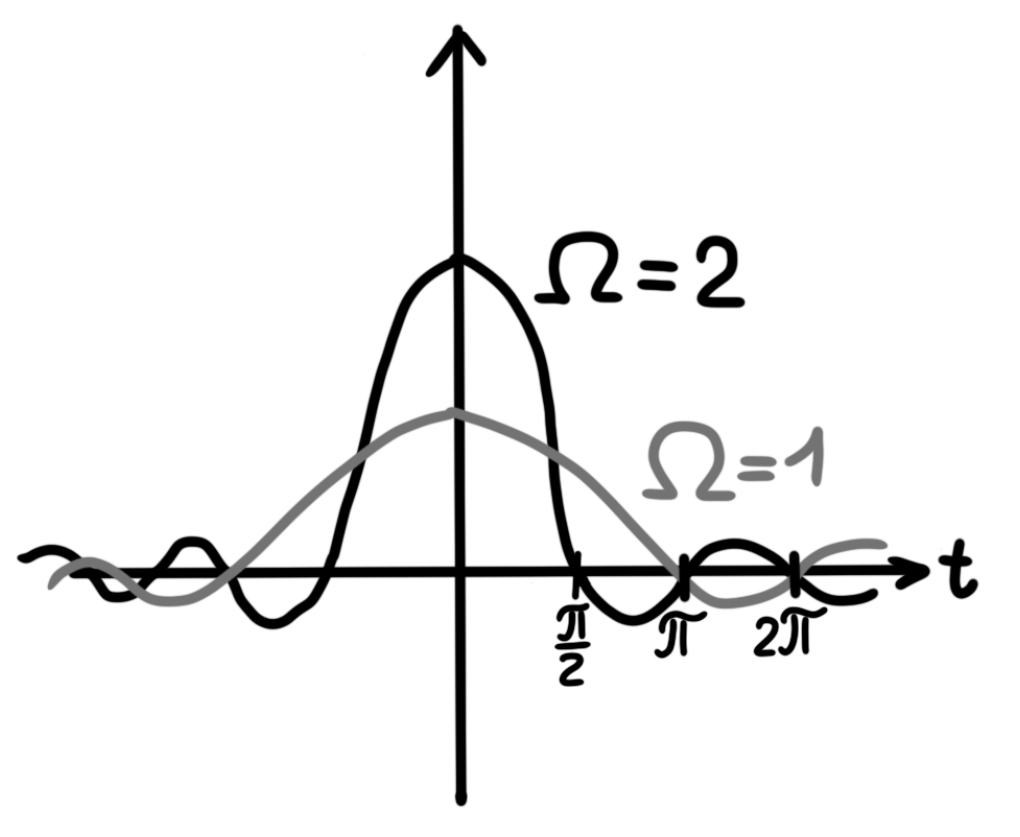
\includegraphics[width=0.4\textwidth]{/Users/vladbelousov/Desktop/Semestr_4-FP-NSU/ЭиО/Лекции_по_дням/image/10.png}
\end{center}

\[ \int_{-\infty }^{\infty} I (t)dt =\lim \int_{-\infty}^{\infty} 2 \Omega \frac{\sin  ( \Omega t)}{\Omega t}dt = 2 \int_{- \infty }^{\infty} \frac{ \sin x}{x}dx = 2 \cdot \mathrm{Im} \left[ \int_{-\infty }^{\infty} \frac{e^{ix} }{x} dx \right]      \] 

\[ \int_{C} \frac{e^{ix} }{x} dx =0 = \underbrace{\int_{|z|= R}}_{=0}  + \int_{-\infty}^{-\rho} + \int_{|z|= \rho} + \int_{ \rho}^{\infty}       \] 

\[ \int_{-\infty}^{\infty} \frac{e^{ix} }{x} dx = - \int_{|z|=\rho} \frac{e^{i \rho e ^{i \varphi} } \cdot \rho i e^{ i \varphi} d \varphi }{\rho e^{i \varphi}} =- i \int_{\pi}^{0} d \varphi= i \pi \Rightarrow \int_{-\infty }^{\infty} I ( t)dt = 2\pi      \] 

\[ \int_{-\infty }^{\infty}  e^{- i \omega t} d \omega = 2 \pi \delta ( t) \quad \int_{-\infty}^{\infty} e ^{ - i \omega t }dt = 2 \pi \delta(\omega)  \]

\[ \int_{-\infty}^{\infty}   e^{- i \omega( t - \tau)} d \omega = 2 \pi \delta ( t - \tau )\quad  \int_{-\infty}^{\infty}    e^{-i (\omega- \omega ') t} d \omega = 2 \pi \delta ( \omega- \omega' )   \] 

1)\[  \delta ( t- \tau )= \frac{1}{ \sqrt{ 2 \pi }} \int_{-\infty}^{  \infty} \underbrace{\frac{1}{ \sqrt{2\pi }} e^{+i \omega t} }_{\delta ( t - \tau) }e^{- i \omega t} d \omega \] 

2)\[ f(t)= \int_{-\infty}^{\infty} f(\tau ) \delta ( t - \tau)d \tau = \int_{-\infty}^{\infty} \frac{f(\tau)d \tau}{2 \pi} \int_{-\infty}^{\infty} e^{- i \omega ( t - \tau ) }d \omega = \frac{1}{ \sqrt{2 \pi}} d \omega e ^{- \omega t } \frac{1}{\sqrt{2 \pi}} \int_{-\infty}^{\infty} d \tau f( \tau) e^{i \omega \tau}       \] 

3) \[ \int_{-\infty}^{\infty}   f_1 ( t)f_2 ^{*}dt  = \int_{-\infty}^{\infty}   dt \frac{1}{\sqrt{2\pi}}\int_{-\infty}^{\infty} \hat{f_1 }(\omega)e ^{-i \omega t} d \omega \frac{1}{\sqrt{2 \pi}} \int _{-\infty}^{\infty} \hat{f_2 }(\omega') e^{i \omega' t} d \omega'    = \]

\[ = \int_{-\infty}^{\infty}    \hat{f_1} (\omega)d \omega \hat{f_2 ^{*} }(\omega') d \omega' \frac{1}{2 \pi} 2\pi \delta ( \omega -\omega') f_1(t)= \int_{-\infty }^{\infty}\hat{f_1 }(\omega) \hat{f_2 ^{*} }(\omega) d \omega  \]

\[ \Rightarrow \int_{-\infty}^{\infty} |f(t)| ^2 dt = \int  _{-\infty}^{\infty} |\hat{f}(\omega)| ^2 d \omega - \text{ равенство Парсеваля }   \] 

\begin{center}
    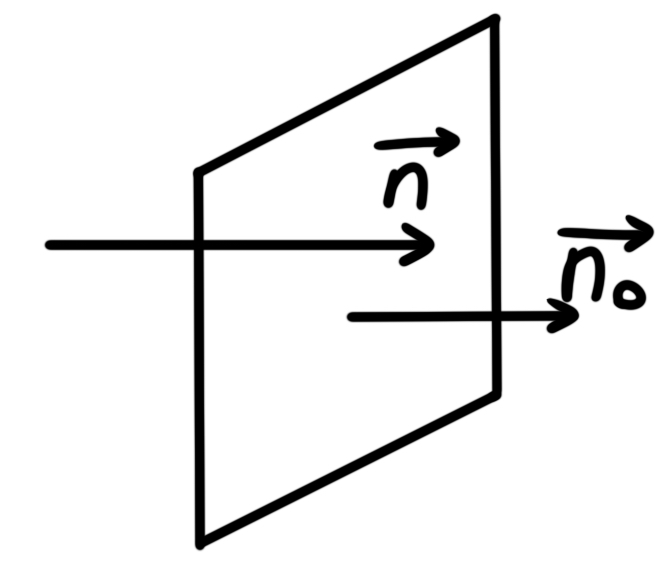
\includegraphics[width=0.2\textwidth]{/Users/vladbelousov/Desktop/Semestr_4-FP-NSU/ЭиО/Лекции_по_дням/image/12.png}
\end{center}

Прошедшая энергия за \( \infty \)  интервал времени через см\( ^2 \)

\[ = \int (\vec{S}\vec{n})dt= \frac{c}{\sqrt{\mu \varepsilon}} \frac{\varepsilon}{ 4\pi }  \int_{-\infty}^{\infty} \vec{E} ^2(t)dt = \frac{c}{\sqrt{\mu \varepsilon}} ( \vec{n}\vec{n_0}) \frac{\varepsilon}{4 \pi} \int_{-\infty}^{\infty} |\hat{\vec{E}}(\omega) | ^2 d \omega  \] 

Свойства Фурье-преобразования: 

1) Пусть \( \displaystyle f(t) \in  \mathbb{R} \Rightarrow f(t)= f^*(t)= \frac{1}{\sqrt{2\pi}}\int_{-\infty}^{\infty} \hat{f^{*} }e ^{+i \omega t} d \omega =[\omega \to  - \omega ']   =  \)

\[ =\frac{1}{\sqrt{ 2 \pi }}(- )\int_{-\infty}^{\infty} d \omega ' \hat{f^{*} } ( -\omega ')e^{- i \omega' t}     \] 

\[ \hat{f^*} (- \omega) = \hat{f}(\omega)  \]

\[ \hat{f^*} ( \omega) = \hat{f}(-\omega) \] 


2) Спектр сдвинутого по времени сигнала:

\begin{center}
    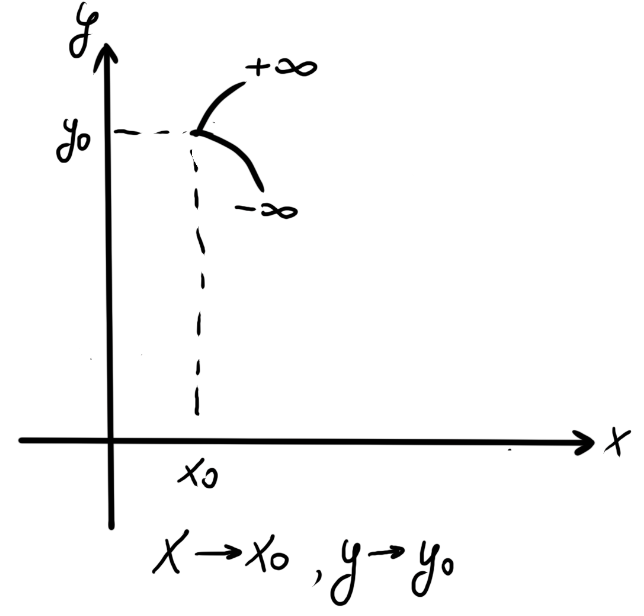
\includegraphics[width=0.5\textwidth]{/Users/vladbelousov/Desktop/Semestr_4-FP-NSU/ЭиО/Лекции_по_дням/image/11.png}
\end{center}
\[  \hat{F}(\omega)=\frac{1}{\sqrt{2 \pi}}\int_{-\infty}^{\infty} f(t- T)e^{+ i \omega t }dt = \frac{1}{\sqrt{2\pi}} \int_{-\infty}^{\infty} f(t' )e^{+ i \omega t } e^{i \omega T} dt =\hat{f}(\omega)e^{i \omega T}         \]  

3) \[  F( t)= f(t) e^{- i \omega_0 t  }\quad  F(\omega)= \frac{1}{\sqrt{2 \pi}} \int_{-\infty}^{\infty}   f(t) e ^{- i \omega_0 t} e ^{i \omega t}dt  = \hat{f}( \omega - \omega_0) \]  

\begin{center}
    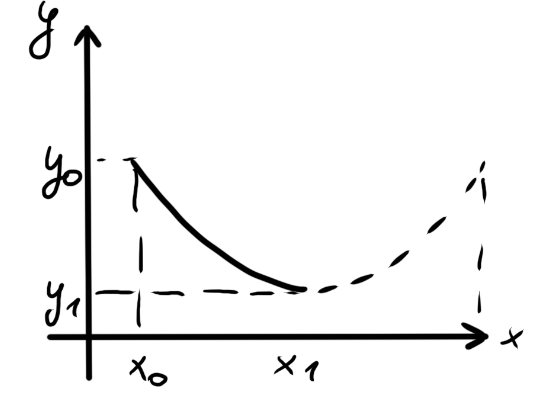
\includegraphics[width=0.5\textwidth]{/Users/vladbelousov/Desktop/Semestr_4-FP-NSU/ЭиО/Лекции_по_дням/image/13.png}
\end{center}

4) Спектр N повторенного сигнала: 

\[ F(t)= \sum_{n=0}^{N-1} f( t - nT); \quad F(\omega)= \sum _{n=0}^{N-1} \hat{f}(\omega) e^{i \omega n T} = f( \omega ) \frac{ e ^{i \omega NT} -1}{e ^{i \omega T} -1}  = \hat{f} ( \omega )= \hat{f}(\omega) e^{i \omega T \frac{ N-1 }{2} } \boxed{\frac{\sin \left( \frac{\omega T}{2}N  \right) }{\sin \left( \frac{\omega T}{2} \right)}}   \]

Последний выделенный  множитель в правой части уравнения - это интерференционный множитель.

\begin{center}
    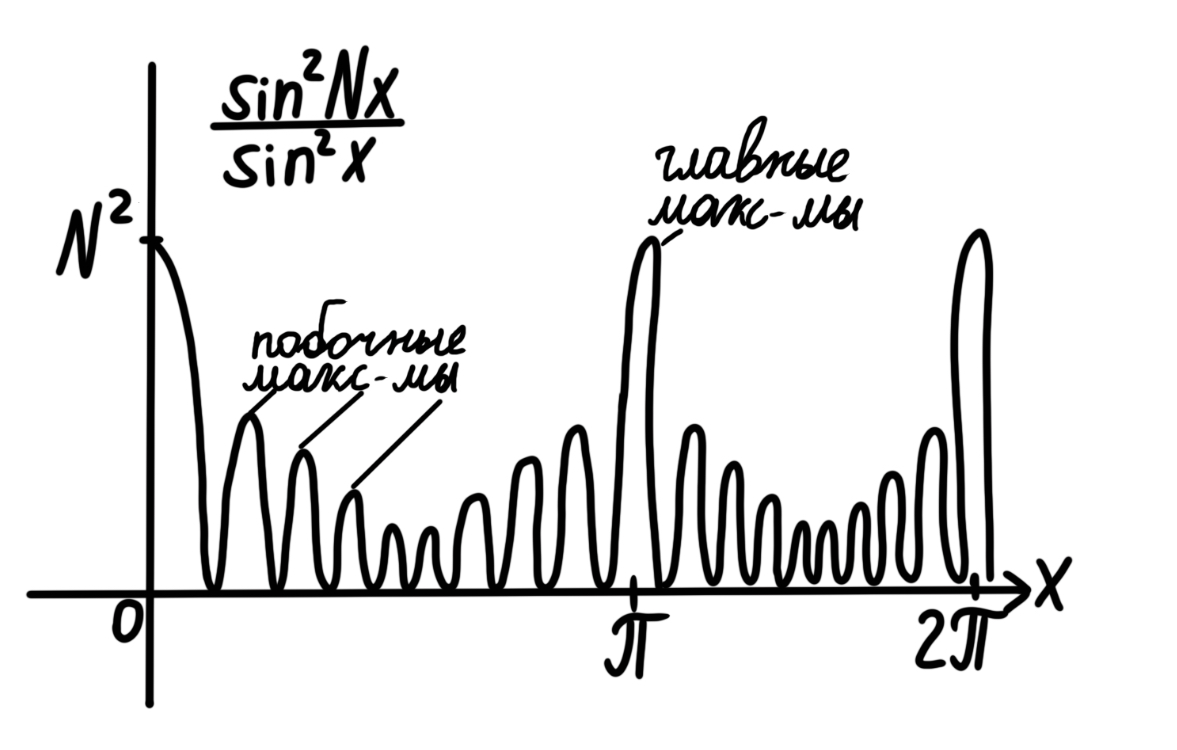
\includegraphics[width=0.5\textwidth]{/Users/vladbelousov/Desktop/Semestr_4-FP-NSU/ЭиО/Лекции_по_дням/image/14.png}
\end{center}
\[ x=  m \pi \varepsilon, \varepsilon > 0  \] 

\[ \frac{\sin ^2 (N ( m\pi+ \varepsilon))}{\sin  ^2 ( m \pi + \varepsilon )} = N ^2   \] 
%%-------------------------------%%


% Закрытие документа, если файл компилируется отдельно
\ifdefined\mainfile
    % Если это основной файл, не нужно заканчивать документ
\else
    \end{document}
\fi
% Условная компиляция для самостоятельной работы
\ifdefined\mainfile
    % Если это часть основного файла, не добавляем начало и конец документа
\else
    \documentclass[12pt, a4paper]{report}
    \usepackage{/Users/vladbelousov/Desktop/Semestr_4-FP-NSU/Настройка/library}
    \usepackage[utf8]{inputenc} % Подключение поддержки UTF-8
    \begin{document}
\fi

%%-------------------------------%%

\section{Продолжение. Спектр свертки двух функций}

\[ F(t)= \int_{-\infty}^{\infty} f(\tau)g(t- \tau)d \tau= \int_{-\infty}^{\infty} d \tau \frac{1}{\sqrt{2 \pi}} \int_{-\infty}^{\infty} \hat{f} (\omega) e ^{- i \omega \tau} d \omega \frac{1}{\sqrt{2\pi}} \int_{-\infty}^{\infty} \hat{g} (\omega') e^{i \omega' (t - \tau)} d \omega'     =\] 

\[ =\int_{-\infty}^{\infty}  d \omega \int_{-\infty}^{\infty} d \omega ' \hat{f} (\omega) \hat{g}(\omega ') e^{- \omega ' t } \frac{1}{2 \pi } \int_{-\infty}^{\infty} \underbrace{d \tau e^{- i (\omega - \omega ' )\tau}}_{=2\pi \delta(\omega- \omega')} = \int_{-\infty}^{\infty}  d \omega \hat{f} ( \omega) \int_{-\infty}^{\infty}  d \omega ' \hat{g} ( \omega ' ) \delta(\omega - \omega ') e ^{-i \omega' t} =        \] 

\[ = \frac{1}{\sqrt{2 \pi}} \int_{-\infty}^{\infty}  \sqrt{ 2 \pi} \hat{f}( \omega ) \hat{g} (\omega   )e ^{- i\omega t}   d \omega \Rightarrow F(t) \risingdotseq \sqrt{ 2 \pi } \hat{f}( \omega ) \hat{g } ( \omega)  \] 

\section{Соотношение неопределенностей}

\begin{definition}
    Определенная связь между длительностью сигнала и шириной его спектра называется соотношение неопределенностей.
\end{definition}

Покажем эту связь на примерах: 

1) Спектр прямоугольного сигнала \( E_1 (t) =\begin{cases}
E_0 , |t| \le  \frac{\tau}{2} \\
0 , |t| > \frac{\tau}{2}
\end{cases} \) E(t) - сигнал.

\begin{center}
    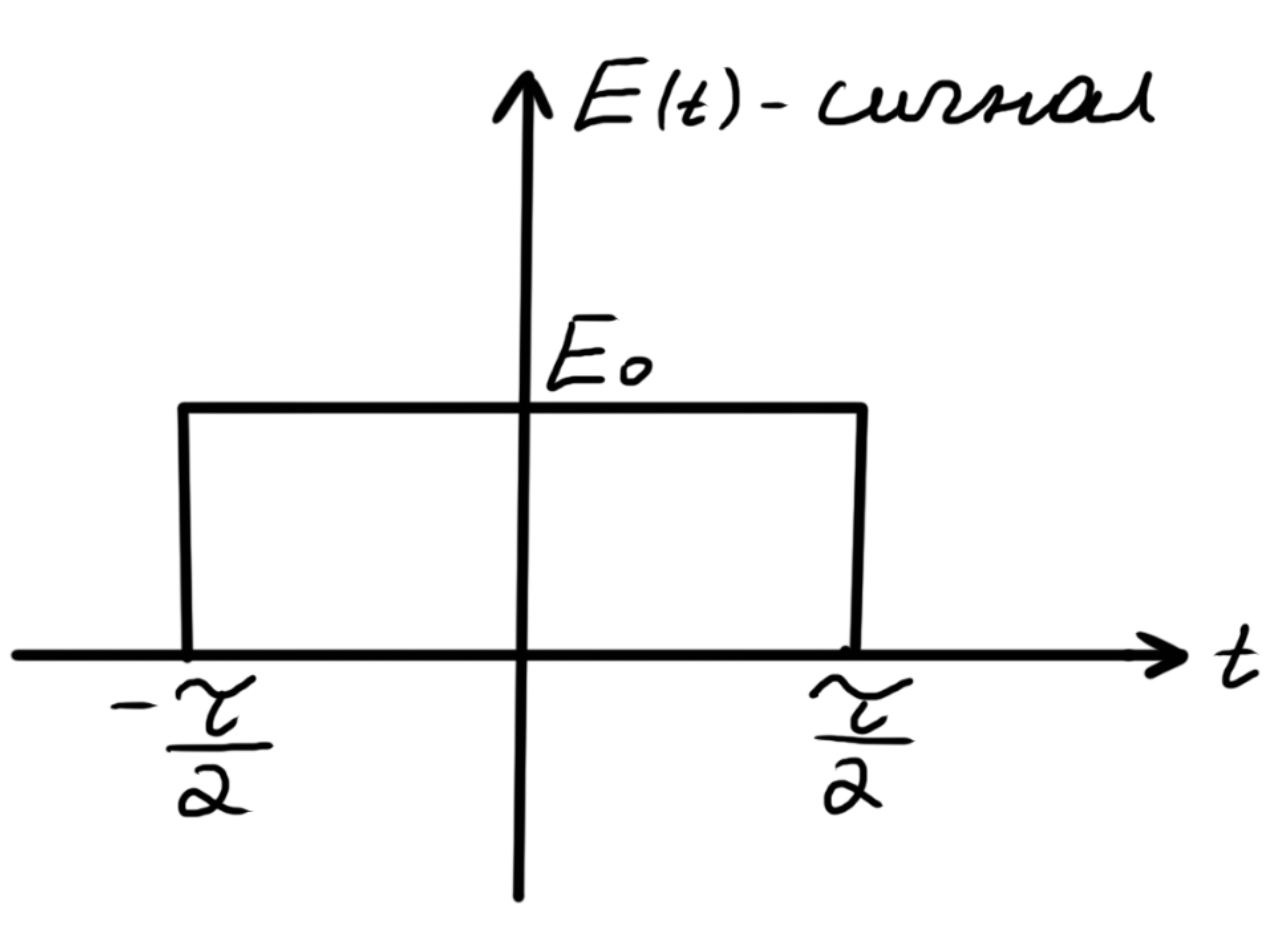
\includegraphics[width=0.3\textwidth]{/Users/vladbelousov/Desktop/Semestr_4-FP-NSU/ЭиО/Лекции_по_дням/image/15.png}
\end{center}

\[ \hat{E}(\omega)= \frac{1}{\sqrt{2 \pi}} \int_{\frac{\tau}{2} }^{-\frac{\tau}{2} } E_0 E^{+ i \omega t} d t = \frac{E_0 \tau}{\sqrt{2 \pi}} \frac{e^{ i \omega \frac{\tau}{2} }- e^{ - i \omega \frac{\tau}{2} }}  {2 i \omega \frac{\tau}{2} }     = \frac{E_0 \tau}{\sqrt{2 \pi}} \mathrm{sinc} ( \frac{\omega \tau}{2} )   \] 

\begin{center}
    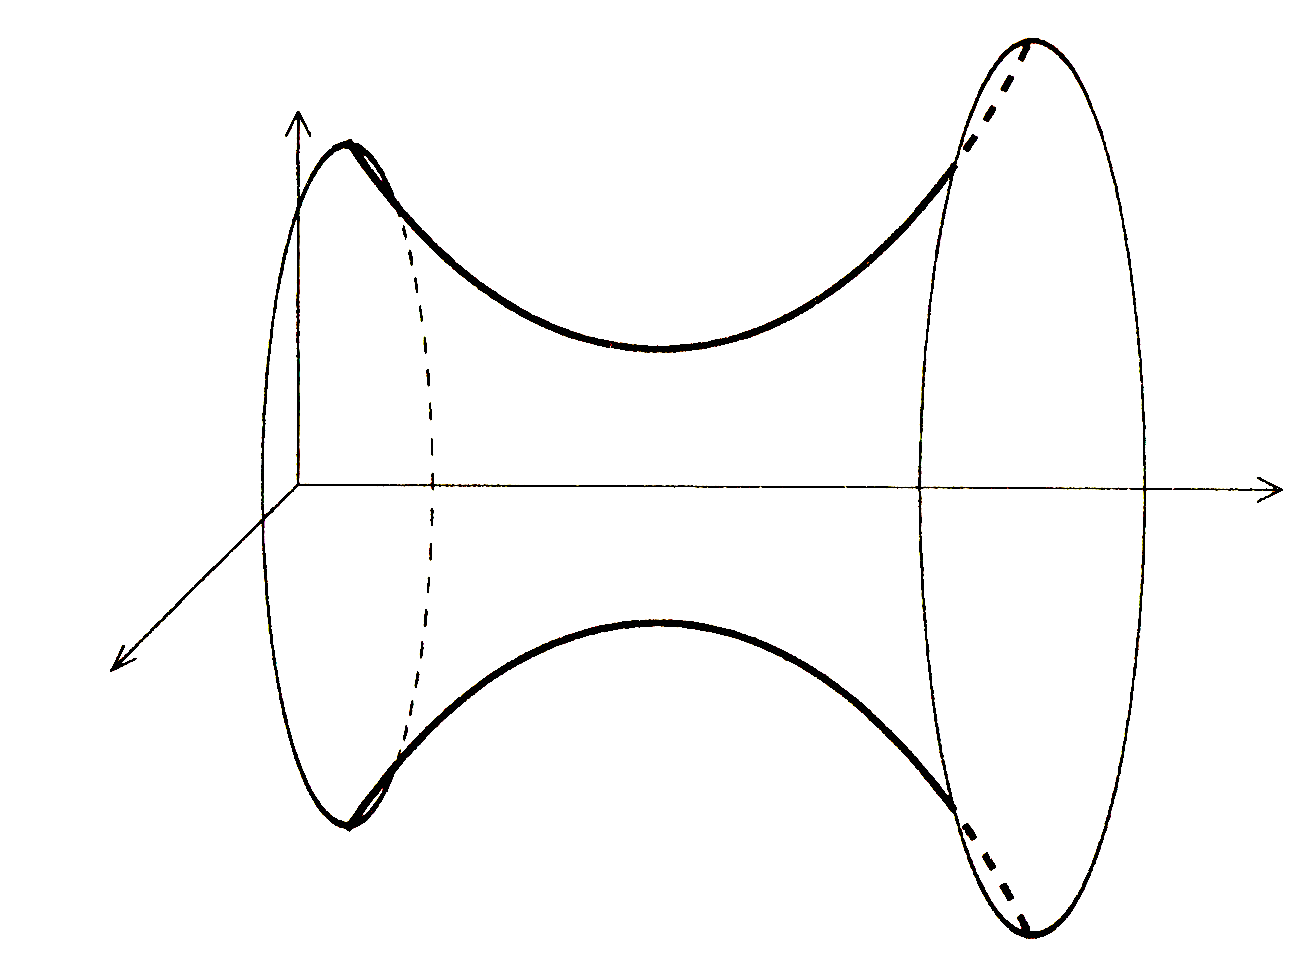
\includegraphics[width=0.5\textwidth]{/Users/vladbelousov/Desktop/Semestr_4-FP-NSU/ЭиО/Лекции_по_дням/image/16.png}
\end{center}

Спектральная плотность энергии = \( |\hat{E } (\omega)| ^2  \) 

\begin{center}
    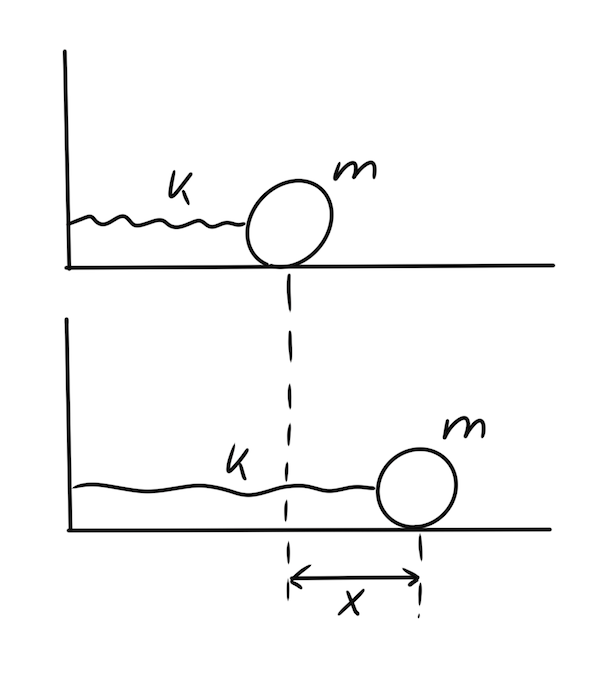
\includegraphics[width=0.5\textwidth]{/Users/vladbelousov/Desktop/Semestr_4-FP-NSU/ЭиО/Лекции_по_дням/image/17.png}
\end{center}

\[ \Delta \omega \sim  \frac{2 \pi}{ \tau} \Rightarrow \Delta \omega \tau \sim \pi - \text{ соотношение неопределенности}     \] 

\[ \tau \to  \infty \Rightarrow \hat{E } \sim  \delta ( \omega)  \] 



2)Спектр синусоидальной волны: 

\[ \begin{aligned}
    E_2 ( t) = \begin{cases}
        E_0 \sin  \omega_0 t , |t| \le \frac{\tau}{2} \\
        0 , |t| > \frac{\tau}{2}
    \end{cases}, 
    \omega_0 = \frac{2 \pi}{\tau} \quad \text{, пусть } \tau= N T , N(\text{целое} ) \gg 1 
\end{aligned} \] 

\begin{center}
    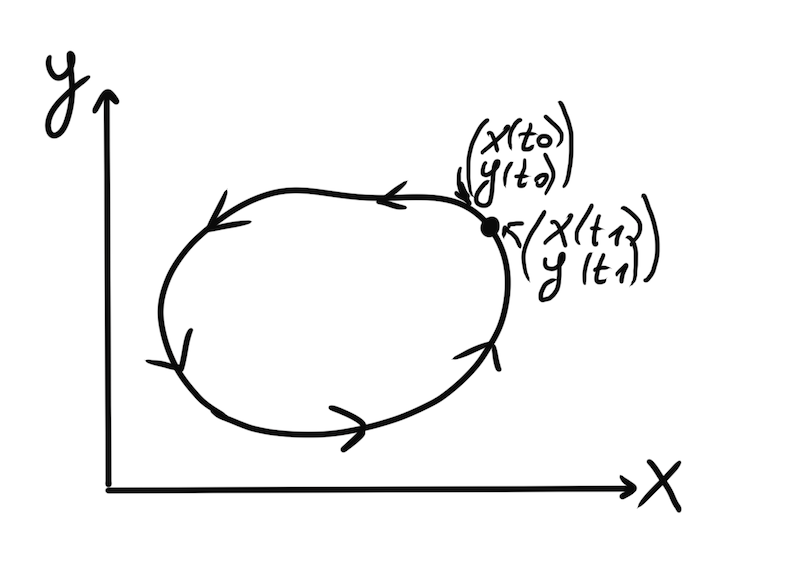
\includegraphics[width=0.5\textwidth]{/Users/vladbelousov/Desktop/Semestr_4-FP-NSU/ЭиО/Лекции_по_дням/image/18.png}
\end{center}


\[ \hat{E_2 } ( \omega) = \frac{1}{ \sqrt{2 \pi}} \int_{-\infty}^{\infty} \frac{ e^{ i \omega_0 t } - e^{- i \omega_0 t} }{2 i} e^{i \omega t} dt  = \frac{1}{2i} \left\{ \frac{E_0 \tau}{\sqrt{2 \pi}}\mathrm{sinc} \left[ (\omega + \omega_0) \frac{\tau}{2}  \right] -    \frac{E_0 \tau}{\sqrt{2 \pi}}\mathrm{sinc} \left[ (\omega - \omega_0) \frac{\tau}{2}  \right]\right\}      \] 

\begin{center}
    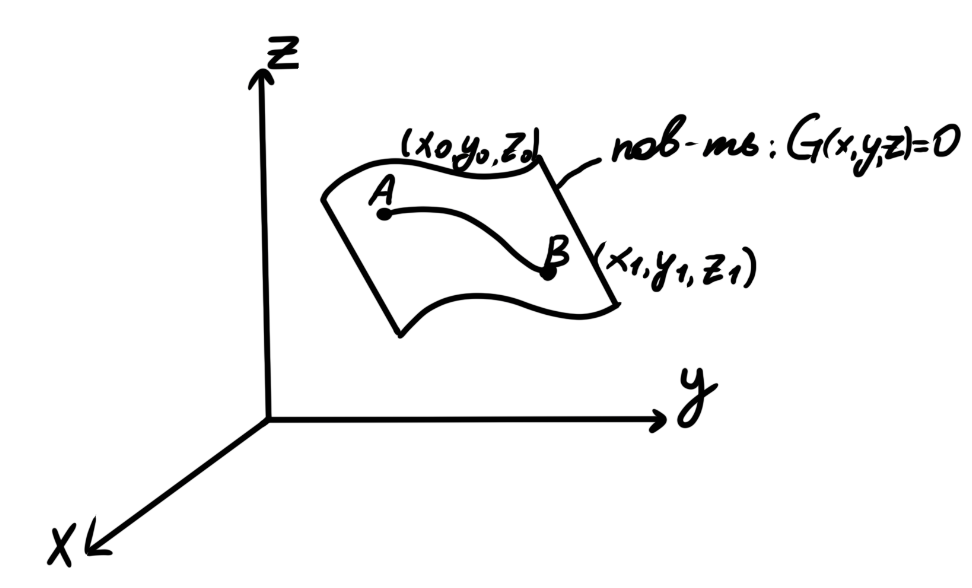
\includegraphics[width=0.45\textwidth]{/Users/vladbelousov/Desktop/Semestr_4-FP-NSU/ЭиО/Лекции_по_дням/image/19.png}
    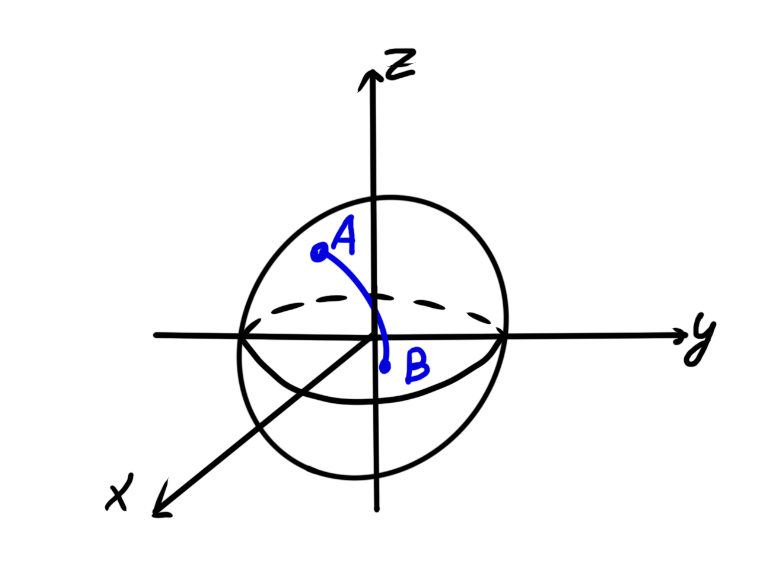
\includegraphics[width=0.45\textwidth]{/Users/vladbelousov/Desktop/Semestr_4-FP-NSU/ЭиО/Лекции_по_дням/image/20.png}
\end{center}

Если \( \frac{\Delta \omega}{\omega_0} \ll 1   \), то такая волна - квазимонохроматическая. 

3) Спектр радиационно затухающего осциллятора:

Механистическая модель атома:

\[ E(t)= \begin{cases}
E_0 e^{ \gamma t} \cos \omega_0 t , t >0\\
0, t < 0
\end{cases} \] 

\[ \gamma = \frac{e ^2 \omega_0 ^2 }{3 m c ^2 } \sim 10 ^9 c^{-1} \quad  \omega_0 \approx 2 \cdot 10^{16} \frac{rad}{c}  \Rightarrow f \sim 3 \cdot 10^8 c^{-1}    \] 

\[ e^{ - \gamma t} = e^{- \frac{t}{\tau} } \Rightarrow \tau \sim \frac{1}{\gamma}      \] 

\begin{center}
    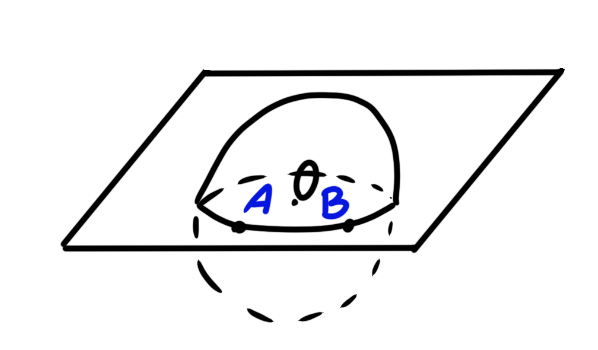
\includegraphics[width=0.5\textwidth]{/Users/vladbelousov/Desktop/Semestr_4-FP-NSU/ЭиО/Лекции_по_дням/image/21.png}
\end{center}

\[ \hat{E} ( \omega ) =\frac{1}{\sqrt{2 \pi}}  \int_{0}^{\infty} E_0 e^{ - \gamma t } \frac{ e^{i \omega_0 t}+ e^{- i \omega_0 t} }{2}  e^{+ i \omega t }   d t     \] 

\[ \hat{E}(\omega) = \frac{E_0}{2 \sqrt{2 \pi}} \left\{ -\frac{1}{- \gamma + i (\omega + \omega_0)}-\frac{1}{- \gamma + i (\omega - \omega_0)}  \right\} = \hat{ f}( \omega + \omega_0) \hat{f}( \omega - \omega_0 )  \]

\[ \lvert \hat{f}(\omega- \omega_0 )   \rvert ^2 = \frac{E_0 ^2 }{8 \pi} \] 

\begin{center}
    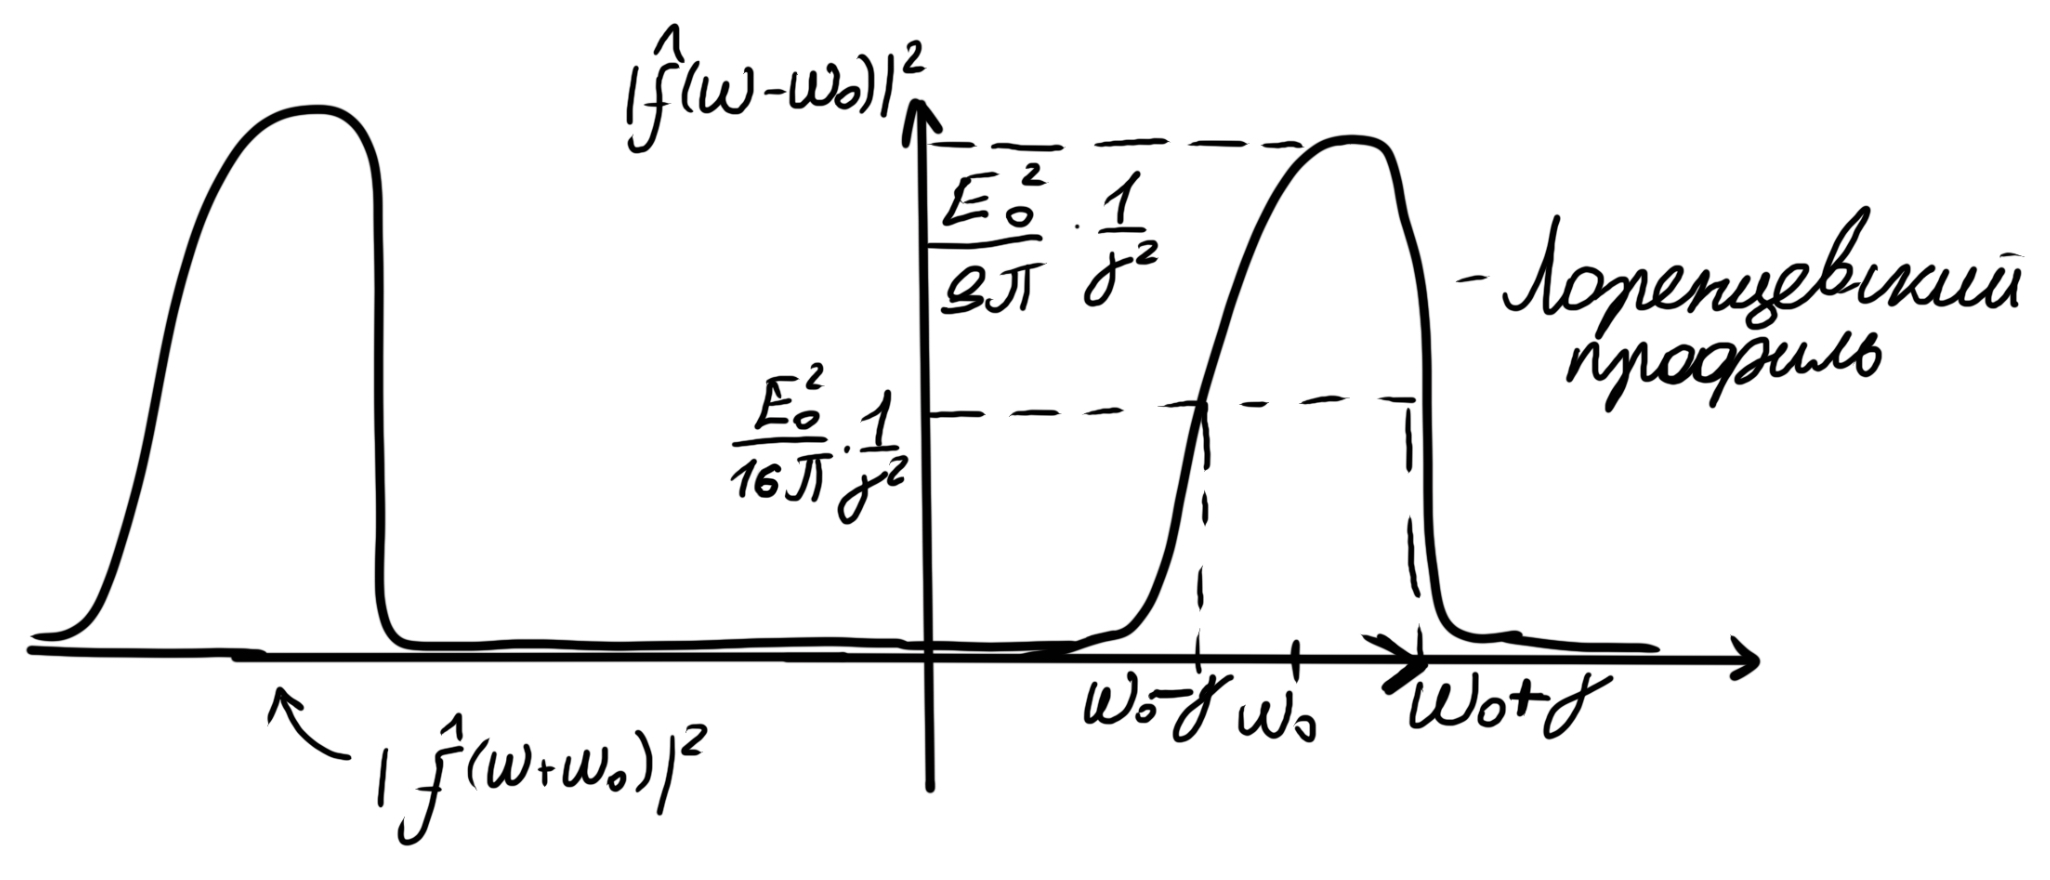
\includegraphics[width=0.55\textwidth]{/Users/vladbelousov/Desktop/Semestr_4-FP-NSU/ЭиО/Лекции_по_дням/image/22.png}
\end{center}

\[ \Delta \omega \sim  2 \gamma - \text{ширина спектра}  \] 

\[ \Delta \omega \underbrace{\Delta t}_{\sim  \tau}  \sim 2 \gamma \frac{1}{\gamma} \sim 2   \] 

\[ |\hat{E} ( \omega ) | ^2 = |\hat{f}(\omega + \omega_0) | ^2 + |\hat{f}(\omega - \omega_0) | ^2 + \cancel{\text{поправка}}  \] 

Поправка  мала, если \( 10^9 c^{-1} \sim\Delta \omega \ll \omega_0 \sim 2 \cdot 10^{16} \frac{rad}{c}  \) 

4) Спектр гауссовой функции : \( f(x) = E_0 e^{ -\alpha x ^2} \quad  \hat{f}( x) = \frac{1}{\sqrt{2 \pi}} \int_{-\infty}^{\infty}   f( x) e^{- i kx }dx =     \) 

\[ \frac{1}{\sqrt{2 \pi}}E_0 \int_{-\infty}^{\infty} e^{- \alpha x ^2 - ikx } dx ; -\alpha x ^2 - ikx = -\alpha \left( x ^2 + 2x \frac{ik}{2 \alpha} - \frac{k ^2}{4 \alpha ^2}   \right) - \frac{k ^2}{4\alpha} =  - \alpha \left( x + \frac{ik}{2\alpha} \right) ^2 - \frac{k ^2}{4\alpha}    \] 

\begin{center}
    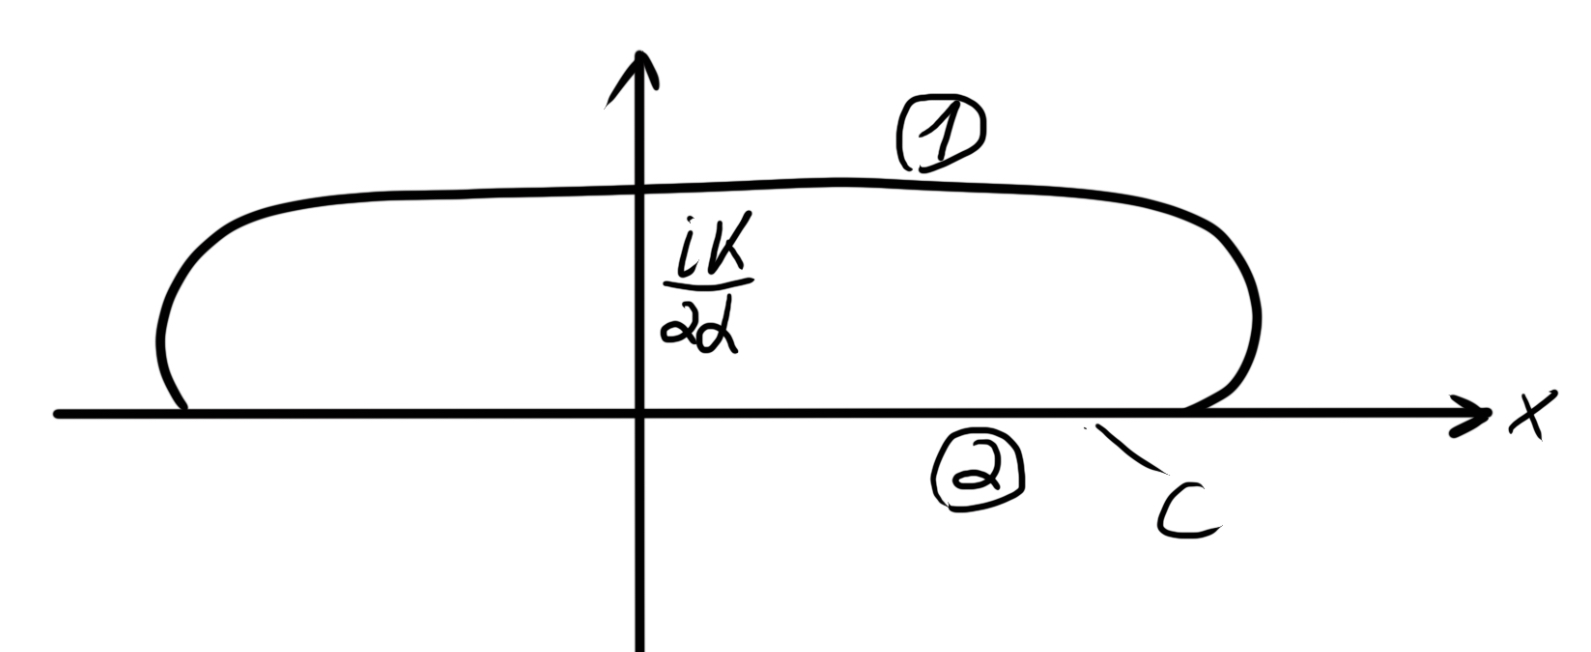
\includegraphics[width=0.4\textwidth]{/Users/vladbelousov/Desktop/Semestr_4-FP-NSU/ЭиО/Лекции_по_дням/image/23.png}
\end{center}

\[  \int_{C} e^{- \alpha z ^2 }dz = 0 = \int_{1} + \int_{ 2} \Rightarrow \int_{1} = \int _{-2}  \] 

\[ \int_{-\infty}^{\infty} e^{-\alpha z ^2 } dz = \int_{-\infty}^{\infty} e^{ - \alpha x ^2 } dx = \sqrt{\frac{\pi}{\alpha} }    \] 

\[ \hat{f} (k) = \frac{ E_0}{\sqrt{2 \pi}} \sqrt{\frac{\pi}{\alpha}} e^{- \frac{k ^2}{4 \alpha} }    \]

\begin{center}
    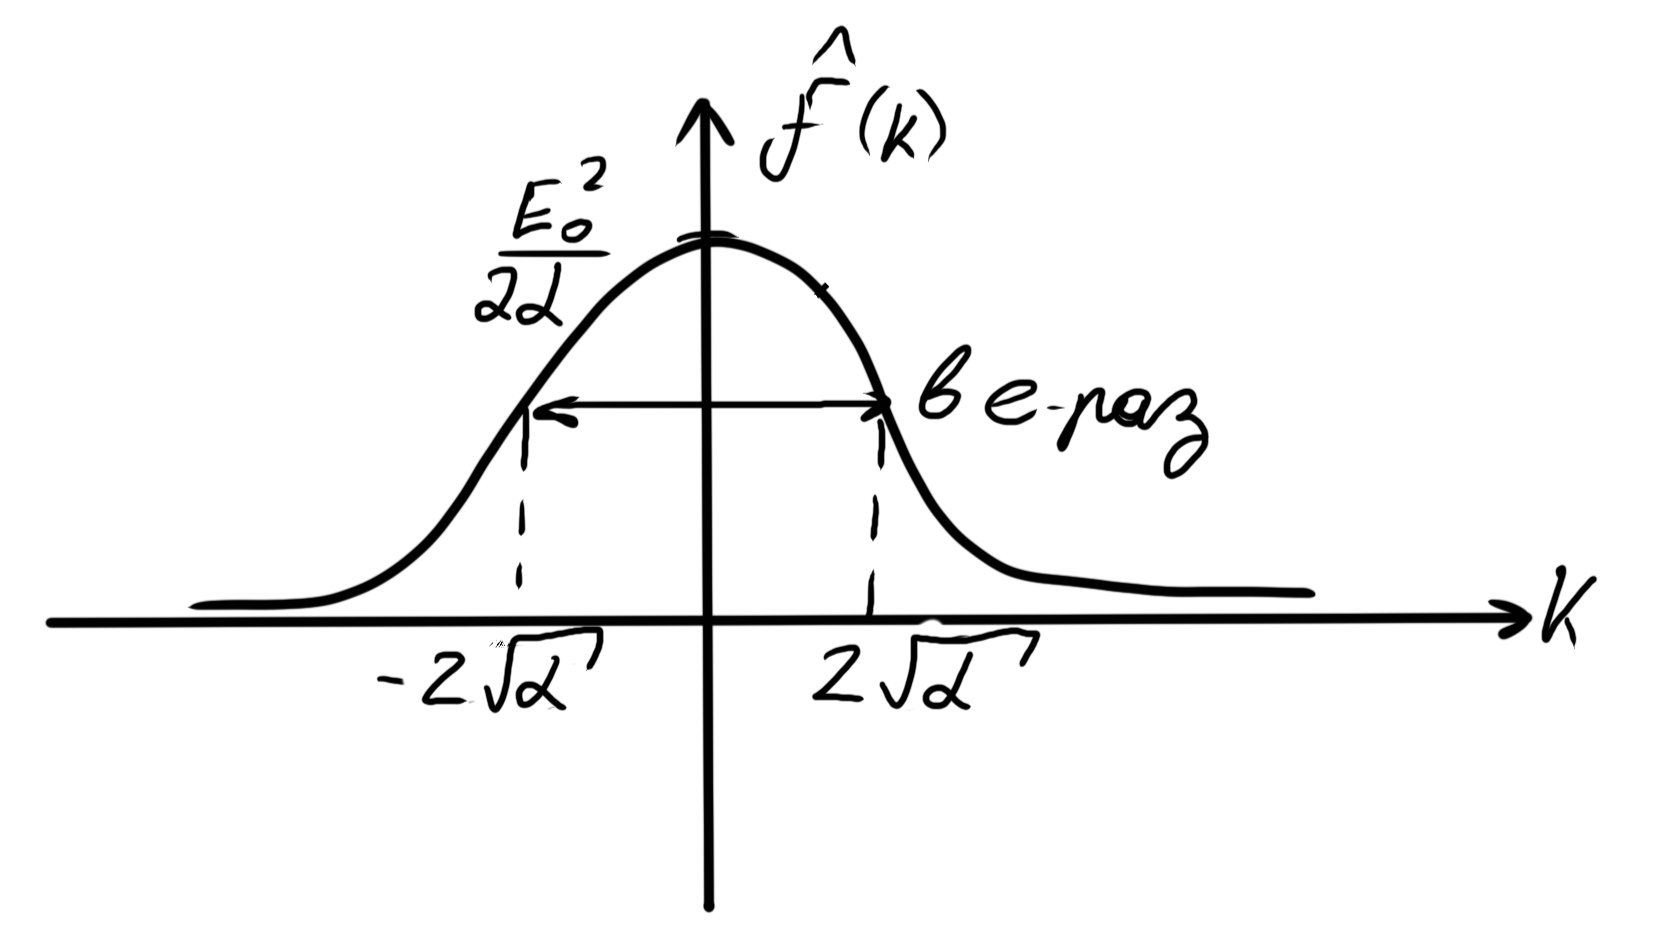
\includegraphics[width=0.45\textwidth]{/Users/vladbelousov/Desktop/Semestr_4-FP-NSU/ЭиО/Лекции_по_дням/image/24.png}
    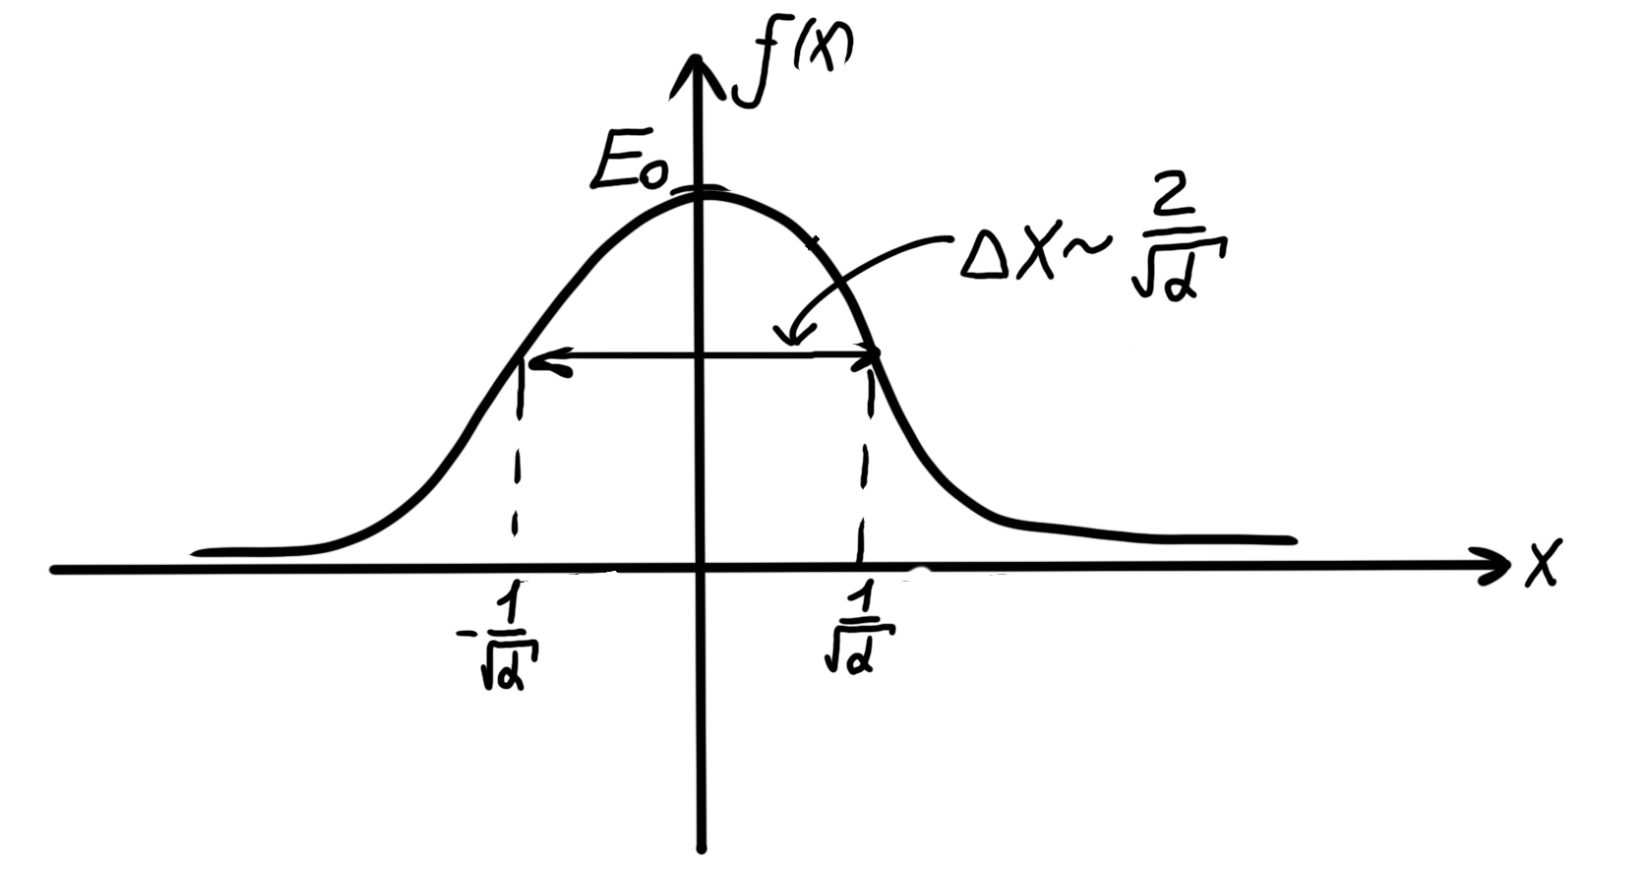
\includegraphics[width=0.45\textwidth]{/Users/vladbelousov/Desktop/Semestr_4-FP-NSU/ЭиО/Лекции_по_дням/image/25.png}
\end{center}


\[\begin{aligned}
    \begin{array}{l}
        \Delta k \sim  4 \sqrt{\alpha} \\
        \Delta x \sim \frac{2}{\sqrt{\alpha}}
    \end{array}
    \Rightarrow 
    \Delta k \Delta x \sim 8 \sim \pi 
\end{aligned} \] 

5) Модулированный гауссиан: \( E(x) = E_0 e^{ - \alpha x ^2} \cos k_0x \) 

\section{Преобразование Фурье функции четырех переменных (x,y,z,t). Уравнения Максвелла в Фурье преобразованиия}

\[ f(x,y,z,t) = \frac{1}{\sqrt{ 2 \pi} ^4} \iiiint \hat{f}(k_x,k_y,k_z,k_t) e^{  i k_x x } e^{ i k_y y } e^{  i k_z z } e^{ - i \omega t } dk_x dk_y dk_z dk_t    \] 

\[ f( \vec{r},t) = \frac{1}{(2 \pi) ^2 } \iiiint \hat{f} ( \vec{k}, \omega) e^{ i( \vec{k},\vec{r})- i\omega t} d^3 k d \omega    \]  

\[ \frac{\partial f( \vec{r},t)}{\partial t} = \frac{1}{( 2 \pi ) ^2} \iiiint \hat{f}(\vec{k}, \omega) ( - i \omega) e^{i \vec{k}\vec{r} - i \omega t} d^3 k d \omega \quad \frac{\partial f}{\partial t}  \risingdotseq   - i \omega \hat{f}( \vec{k}, \omega)    \] 

\[ \frac{\partial f (\vec{r},t)}{\partial x} \risingdotseq i k_x \hat{f}( \vec{k}, \omega) \]

\[ \mathrm{div} \hat{\vec{D}}(\vec{r},t) = \frac{\partial \hat{\vec{D_x}}}{\partial x} + \frac{\partial \hat{\vec{D_y}}}{\partial y} + \frac{\partial \hat{\vec{D_z}}}{\partial z} \risingdotseq i k_x \hat{D_x}(\vec{k}, \omega) + i k_y \hat{D_y}(\vec{k}, \omega) + i k_z \hat{D_z}(\vec{k}, \omega)  = i (\vec{k},\hat{\vec{D}}(\vec{r}, \omega) ) \] 

\[ \mathrm{rot}\hat{\vec{E}}  = [\nabla \times  \hat{\vec{E}} ] = \frac{1}{( 2 \pi ) ^2 } \iiiint \underbrace{\left[ (\nabla \times  \hat{\vec{E}} (\vec{k}, \omega)e^{i (\vec{k}\vec{r}) }   ) \right]}_{\nabla e^{i (\vec{k }, \vec{r })}   \times \vec{E } (\vec{k },\omega) }   e^{- i \omega t } d ^3 d \omega  =      \] 

\begin{center}
    Где \(\nabla e^{i (\vec{k }, \vec{r })} = \vec{e_x }i k_xe^{(i (\vec{k }, \vec{r }))}+ \vec{e_y } i k_y e^{(i (\vec{k }, \vec{r }))} + \vec{e_z } i k_z e^{(i (\vec{k }, \vec{r }))}= i\vec{k } e ^{ i ( \vec{k } , \vec{r})} \)    
\end{center}


\[= \frac{1}{( 2 \pi) ^2 } \iiiint \left[ i \vec{k} \times  \hat{\vec{E }}( \vec{k }, \omega)  \right] e^{i(\vec{k}, \vec{r})- i \omega t} d ^3 k d \omega \] 

\[ \mathrm{rot} \vec{ E }  \risingdotseq i \left[ \vec{k} \times \hat{\vec{E}}(\vec{k}, \omega) \right]   \] 
 
\[ 
\begin{cases}
        \displaystyle \mathrm{rot} \vec{ E } = - \frac{1}{c} \frac{ \partial \vec{B}}{ \partial t} \risingdotseq i \left[ \vec{k } \times \hat{\vec{E}} ( \vec{k }, \omega)  \right] = \frac{i \omega}{c} \hat{\vec{B } } ( \vec{k }, \omega)     \\
        \displaystyle \mathrm{rot} \vec{H} = \frac{ 4 \pi }{ c} \vec{j } + \frac{1}{ c  }  \frac{ \partial \vec{ D } }{ \partial t } \risingdotseq  i \left[ \vec{k } \times \hat{\vec{H}} ( \vec{k }, \omega) \right] = \frac{  4 \pi }{ c } \hat{\vec{j}} ( \vec{k }, \omega)  - \frac{ i \omega }{c } \hat{ \vec{D} } ( \vec{k }, \omega)        \\
        \displaystyle \mathrm{div} \vec{D } = 4 \pi \rho \risingdotseq i ( \vec{k }, \hat{\vec{D}} ( \vec{k }, \omega) ) = 4 \pi \hat{\rho}  ( \vec{k }, \omega)   \\
        \displaystyle \mathrm{div} \vec{B} = 0 \Rightarrow (\vec{k },\hat{\vec{B}} ( \vec{k }, \omega)) = 0    \\
\end{cases}
\] 

В системе слева это уравнения Максвелла, а справа преобразование Фурье уравнений Максвелла.


\[ \frac{ \partial \rho }{ \partial t } + \mathrm{ \div  } \vec{ j }  = 0 \risingdotseq - i \omega \hat{ \rho } ( \vec{k }, \omega) + i ( \vec{k }, \hat{\vec{j}} ( \vec{k }, \omega) ) = 0      \] 

Если \( \vec{B} = \mu \vec{H } , \vec{D } = \varepsilon \vec{ E } , \varepsilon , \mu  - \mathrm{const}   \)

\[ \underset{a}{\vec{k}} \times \left[ \underset{b}{\vec{k} }\times \underset{c}{\vec{E}}  \right] = \frac{\omega \mu}{c }  \left( - \frac{\omega}{ c } \varepsilon \hat{\vec{E}}  \right)
\] 
\( \quad \quad \quad \quad \quad \quad \quad \quad \quad \quad \quad \quad \quad \quad || \) 

\[ \vec{k } \underbrace{( \vec{k }, \hat{\vec{E }})}_{=0} - \hat{ \vec{ E } } k ^2 = - \frac{\varepsilon \mu }{c ^2 } \omega ^2 \hat{\vec{E }} \Rightarrow k ^2 = \frac{ \omega ^2 }{\left( \frac{c}{\sqrt{\varepsilon \mu}}      \right) ^2} = \frac{\omega ^2 }{v ^2 _{\text{в} } }       \] 


%%-------------------------------%%

% Закрытие документа, если файл компилируется отдельно
\ifdefined\mainfile
    % Если это основной файл, не нужно заканчивать документ
\else
    \end{document}
\fi


% Условная компиляция для самостоятельной работы
\ifdefined\mainfile
    % Если это часть основного файла, не добавляем начало и конец документа
\else
    \documentclass[12pt, a4paper]{report}
    \usepackage{/Users/vladbelousov/Desktop/Semestr_4-FP-NSU/Настройка/library}
    \usepackage[utf8]{inputenc} % Подключение поддержки UTF-8
    \begin{document}
\fi

%%-------------------------------%%


\section{Материальные уравнения в Фурье-представлении}

\[ \frac{d \vec{p } }{dt } = - k \vec{r }_e (t )+ e \vec{r }_e (t )  \] 

\( \frac{d \vec{ r } _e }{dt }= \frac{\vec{ p } }{\gamma m }   \Rightarrow \text{ в }  \vec{r } _e (t ) \)   в следствие инерции электрона аккумулируется история (память) о воздействии.

Электрическим полем в предыдущие моменты времени \( t' \)  ,  а \( \vec{r } _e        \) дает вклад в \( \vec{P } (r,t) \). В общем случае линейная связь \( \vec{D }     \)  и \( \vec{E}  \)  полей имеет вид: 

\[ \vec{D } (\vec{r } ,t )= \vec{E } (\vec{r } , t )+ 4 \pi \vec{P } (\vec{r } , t ) = \frac{1}{(2 \pi ) ^2 } \iiiint \varepsilon(\vec{r } , \vec{r '} , t ,t ' ) \vec{E } (\vec{ r' } ,t' ) d ^3 r ' dt ' \quad ( t '< t ) \] 

Зависимость \( \varepsilon  \)  от \( \vec{r ' }  \)  возникает в случае переноса в веществе заряженных частиц (или обладающих дипольным моментом) из других точек среды.

Упрощения: 

1) Если среда стационарная и ее свойства зависят только от \( \vec{E }       \)  и \( \vec{ H}  \) и ни от ничего другого, то \( \varepsilon ( \vec{r } ,\vec{r '} , t,t ' ) =\varepsilon ( \vec{r } ,\vec{r ' } ,t -t ')  \) 

2) Если среда однородная \( \varepsilon ( \vec{r } ,\vec{r ' } ,t ,t' ) =\varepsilon ( \vec{r } - \vec{r' } , t ,t') \) 

Если среда однородная и стационарная, то 

\[ \vec{D } ( \vec{r } ,t )= \frac{1}{(2 \pi ) ^2 } \iiiint \varepsilon ( \vec{r }- \vec{r '} , t - t' ) \vec{E }  ( \vec{r' } ,t ') d ^3 r ' d t' \text{ (свертка)}    \] 

Используем преобразование Фурье на \( \vec{D}  \) :

\[ \hat{\vec{D } }(\vec{k } ,\omega )=  \hat{\varepsilon}( \vec{k } , \omega ) \hat{\vec{E }}   ( \vec{k}, \omega ); \quad \hat{\vec{B} } ( \vec{k } , \omega ) = \hat{\mu } ( \vec{k } , \omega) \hat{\vec{H }}  (\vec{k }  , \omega) \] 

% Сами в уравнение Максвелла подставите 

\( \displaystyle \frac{\omega ^2 }{c ^2 }\hat{\varepsilon}  (\vec{k } , \omega )\hat{\mu} ( \vec{k } , \omega)= k ^2 \)    - дисперсионное уравнение \( \to       \)   связь \( \omega   \) и \( \vec{k }  \) в среде.

Далее рассматриваем только твердое тело \( \Rightarrow  \varepsilon  \) и \( \mu     \)  зависят только от \( \omega \) 

\[ \frac{\omega ^2 }{c ^2 } \varepsilon( \omega ) \mu ( \omega) = k ^2   \] 

\( \underset{\text{без док-ва} }{\text{Для плазмы } } \)  \( \displaystyle \varepsilon ( \omega ) \simeq 1- \frac{\omega _p ^2 }{\omega ^2 } , \text{ } \omega _ p ^2 = \frac{4 \pi n_p e ^2 }{m } , \text{ } \mu ( \varepsilon ) = 1    \) 

\[ \frac{\omega ^2 }{c ^2 } \left(  1 - \frac{\omega _p ^2}{\omega ^2 }  \right) =k ^2 \Rightarrow \omega ^2 = \omega_p ^2  + k ^2 c ^2   \] 

\begin{center}
    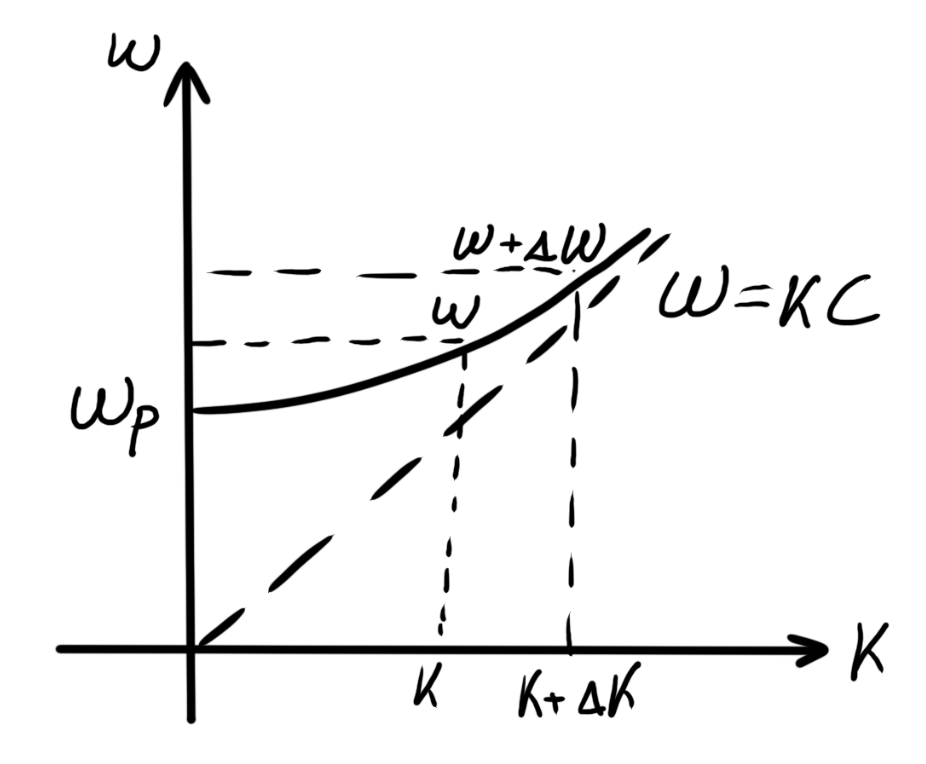
\includegraphics[width=0.4\textwidth]{/Users/vladbelousov/Desktop/Semestr_4-FP-NSU/ЭиО/Лекции_по_дням/image/26.png}
\end{center}

\section{Частотная дисперсия показателя преломления сред. Фазовая групповая скорость}

\[ \vec{E } (z,t ) = \vec{E_0 }e^{ikz - i \omega t }  , \text{ где } \frac{\omega ^2 }{c ^2 }\varepsilon ( \omega )\mu( \omega ) =k ^2    \] 

\( e^{ikz - i \omega t }=e^{ik(z- \frac{\omega}{k } t  )} ;   \) фаза волны \( kz - \omega t = \varphi( z, t ) \) 

\[ \varphi ( \vec{r } , t ) = ( \vec{k }  , \vec{r }  ) - \omega t  \] 

Если фаза \(\displaystyle  \varphi( z , t ) -  \) const, то  \( \displaystyle \frac{dz}{dt } = \frac{\omega}{k } = v_{\text{волны} } = \frac{c}{\sqrt{\varepsilon (\omega ) \mu ( \omega)}} =\frac{c}{ n ( \omega)}   \)

\( n ( \omega ) \) - показатель преломления среды. 

Ни энергия, ни информация не передается с \( v_{\Phi  }  \) (\( v_{\Phi  }  =v_{\text{волны} } \)), которая может быть больше \( c \) 

Рассмотрим монохроматическую волну, состоящую из двух монохроматических плоских волн, с близкой частотой: 

\[ \vec{E }  (z, t ) = \vec{E_0 }(\cos (kz - \omega t )+ \cos  ( (k+ \Delta k)z - ( \omega +\Delta \omega )t))=\]

\[ = \vec{E_0 } 2 \cos \left( \left( k+ \frac{\Delta k}{2}  \right)z - \left( \omega + \frac{\Delta \omega}{2}  \right) \right) \cos \left(  \frac{\Delta k }{2} z - \frac{\Delta \omega }{2 }  t   \right), \quad t=\text{const }     \] 

\begin{center}
    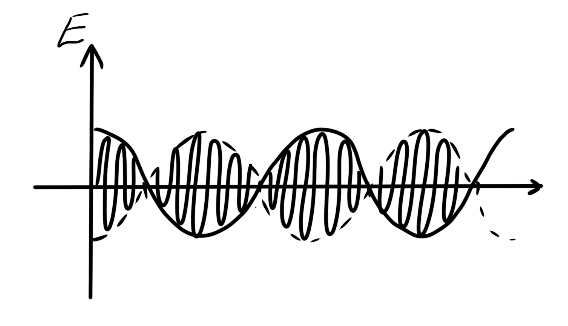
\includegraphics[width=0.5\textwidth]{/Users/vladbelousov/Desktop/Semestr_4-FP-NSU/ЭиО/Лекции_по_дням/image/27.png}
\end{center}

Скорость движения огибающей: 

\[ \frac{\Delta k z }{ 2 }  - \frac{\Delta \omega t }{2 }  = \mathrm{const }  \Rightarrow \frac{dz}{dt } = \frac{ \Delta \omega }{\Delta k } = \boxed {\frac{d \omega }{ dk }  = v_{g}} - \text{ групповая скорость}     \] 

Соотношения Рэлея \( \displaystyle \frac{\omega n( \omega)}{c }  = k \text{ (дисперсионное уравнение)} \Rightarrow   \) 

\[ \frac{d}{d \omega} ( \omega n ( \omega)) = \frac{ dk c }{d \omega } \] 

\[  n(\omega ) + \omega \frac{dn( \omega )}{d \omega } = \frac{dk}{d \omega } c \Rightarrow   \frac{d \omega } {dk } = \frac{ c }{ n( \omega ) + \omega \frac{ dn (\omega)}{d \omega} }  =       \] 

\[ =\underbrace{ \frac{c}{ n ( \omega )}}_{v_{\Phi } } \frac{1}{ 1+ \frac{\omega}{n ( \omega )}\frac{dn}{d \omega}  }  \Rightarrow v_g = \frac{v_{\Phi} } {1+ \frac{\omega}{ n } \frac{dn}{d \omega}  }   \] 

Если \( \displaystyle  \frac{dn}{d \omega }> 0   \) , то \( v_g< v_{\Phi}  \) - нормальная дисперсия

Если  \( \displaystyle  \frac{dn}{d \omega }< 0   \) , то \( v_g>v_{\Phi}  \) - аномальная дисперсия

\section{Движение одномерного волнового пакета в среде с дисперсией \( \omega = \omega( k ) \) }

Известно, что он движется по \( z \) 

\begin{center}
    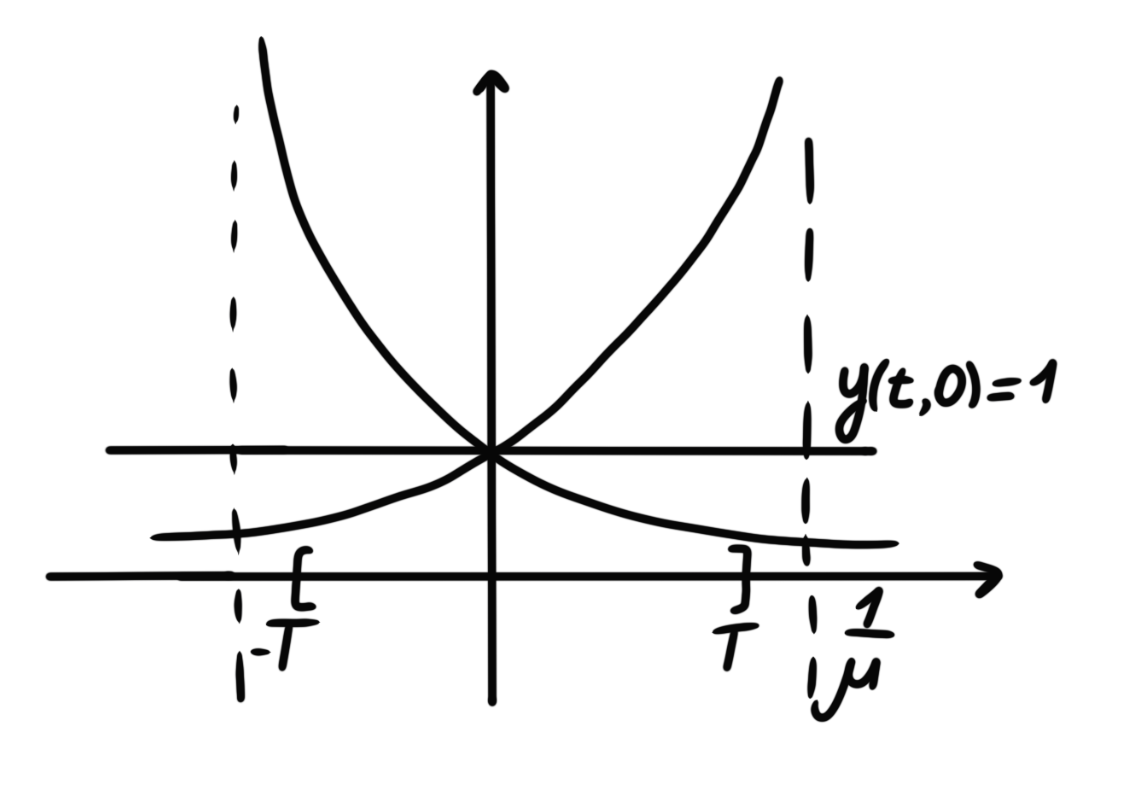
\includegraphics[width=0.5\textwidth]{/Users/vladbelousov/Desktop/Semestr_4-FP-NSU/ЭиО/Лекции_по_дням/image/28.png}
\end{center}

\[ \vec{E } ( z, 0 )= \vec{E_0 } ( z ) e^{i k_0 z}   \]

Используем преобразование Фурье на \( \vec{E}  \): 

\[ \hat{\vec{E }}   ( k ) =\frac{1}{\sqrt{2 \pi } } \int_{-\infty}^{\infty} \underbrace{\vec{E_0}  (z ) e^{i k_0 z }}_{=\vec{E }  (z,0)} e^{- ik z } dz =\hat{ \vec{E_0}  }( k- k_0 )      \] 

Для электрического поля волны с \( k  \)  эволюция во времени описывается: 

\[ \vec{E }  ( k ) e^{ikz - i\omega(k ) t }  \] 

\[ \vec{E }  ( z, k  ) =\frac{1}{\sqrt{2 \pi}}  \int_{-\infty}^{\infty} \vec{E }  ( k ) e^{ikz - i\omega(k ) t }   dk\] 

\begin{center}
    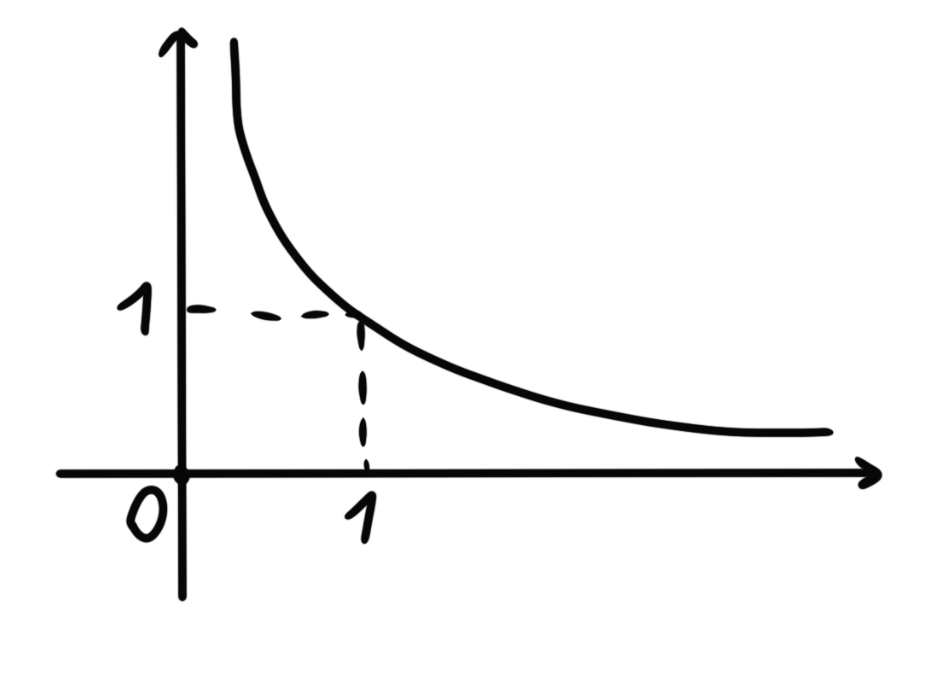
\includegraphics[width=0.5\textwidth]{/Users/vladbelousov/Desktop/Semestr_4-FP-NSU/ЭиО/Лекции_по_дням/image/29.png}
\end{center}

Если \(\displaystyle  \lambda = \frac{2\pi}{k_0} \ll   \) масштаб изменения \( E_0(z ) \) или длины пакета \( L_0 \)  

\begin{center}
    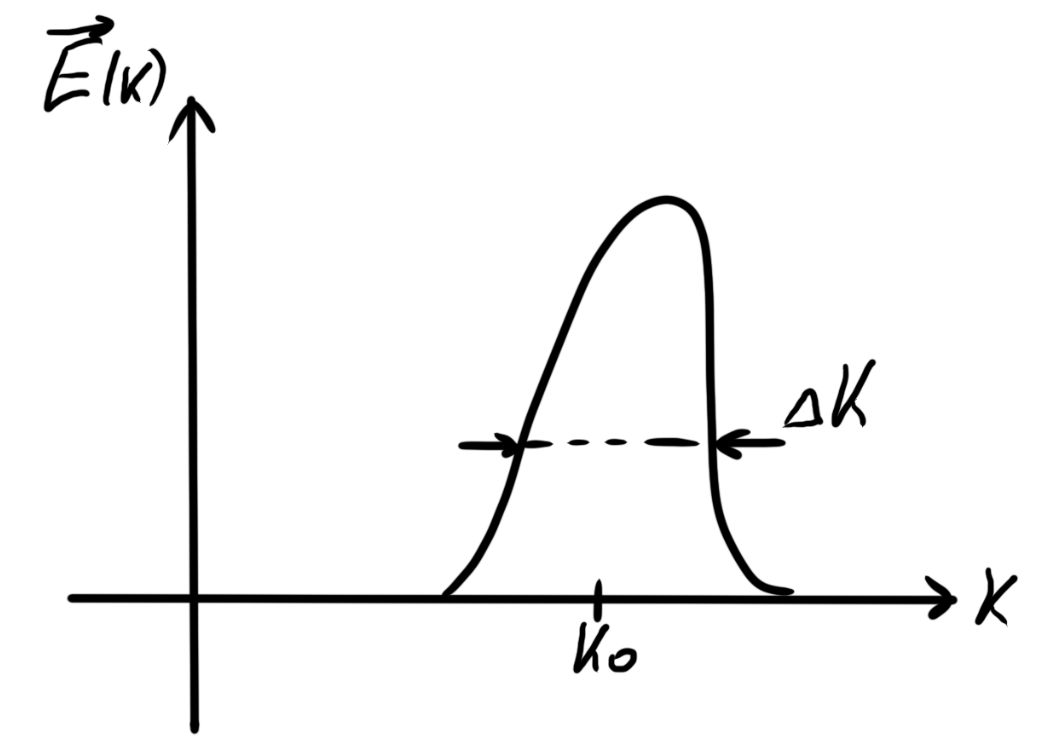
\includegraphics[width=0.5\textwidth]{/Users/vladbelousov/Desktop/Semestr_4-FP-NSU/ЭиО/Лекции_по_дням/image/30.png}
\end{center}

\[ \Delta k L_0 \sim \pi \Rightarrow \Delta k \sim \frac{\pi}{L_0}   \] 

\[ k \sim k_0 \sim \frac{2 \pi }{\lambda} \Rightarrow \frac{\Delta  k }{k_0 } \ll 1     \] 

%рис

\[ \omega ( k ) \simeq \underbrace{\omega( k_0 )}_{\omega_0} + \frac{d \omega }{ dk} \bigg|_{k_0}  (k- k_0 ) + \cancelto{0_{\text{т.к мал} } }{\frac{1}{ 2 }  \frac{ d ^2 \omega } { d k ^2 }  \bigg|_{k_0}  (k-k_0 ) ^2}     \] 

1) Пусть \(\displaystyle  \omega ( k ) = \omega_0 + v_g ( k-k_0 ) ; \vec{E } ( z,t ) = \frac{1}{\sqrt{2 \pi } } \int_{-\infty}^{\infty}  \vec{E }  ( k ) e^{ikz - \omega_0t - i v_gt ( k-k_0)}  dk = \) 

\[ \frac{ e^{i k_0 v_gt -i \omega t} }{\sqrt{2\pi } }\int_{-\infty}^{\infty}  E(k ) e ^{i k (z- v_gt )}dk  = e^{i k_0 v_gt - i \omega_0 t} \vec{E_0} ( z- v_gt ) e^{i k_0 (z- v_gt )}= \vec{E_0} ( z- v_gt  ) e^{i k_0 z - i \omega_0 t }        \] 

- пакет без изменения формы движется по z 

2) Учтем \( \displaystyle i\frac{d ^2\omega }{dk ^2 } \bigg |_{k = k_0}  \frac{(k-k_0 ) ^2 }{2} \Delta t  \ll i \frac{\pi}{2 }  \Rightarrow \Delta t = \frac{\pi}{\Delta k ^2 \omega ''}\sim \frac{ L_0 ^2 }{ \pi \omega ''}        \) 

Если \( \displaystyle t \gg \Delta t    \quad  \frac{\Delta v_g }{\Delta k } \sim \frac{d v_g }{dk } = \frac{d \left( \frac{d \omega}{dk}  \right)}{dk}= \omega '' (k_0 ) \Rightarrow \Delta v_g \simeq \omega '' (k_0 )\Delta k       \) 

Расплывания пакета: \( \Delta L= \Delta v_g t \simeq \omega '' ( k_0 ) \Delta k t   \) 

\[ L(t  ) \simeq \sqrt{L_0 ^2 + \Delta L  ^2 } = \sqrt{ L_0 ^2 + ( \omega '' (k_0  )\Delta k t) ^2 }   \] 

Примеры дисперсионных соотношений: 

1) Электромагнитна волна, в вакууме, звук в среде \( \omega = k a , \text{ }  a = \mathrm{const}   \) 

\begin{center}
    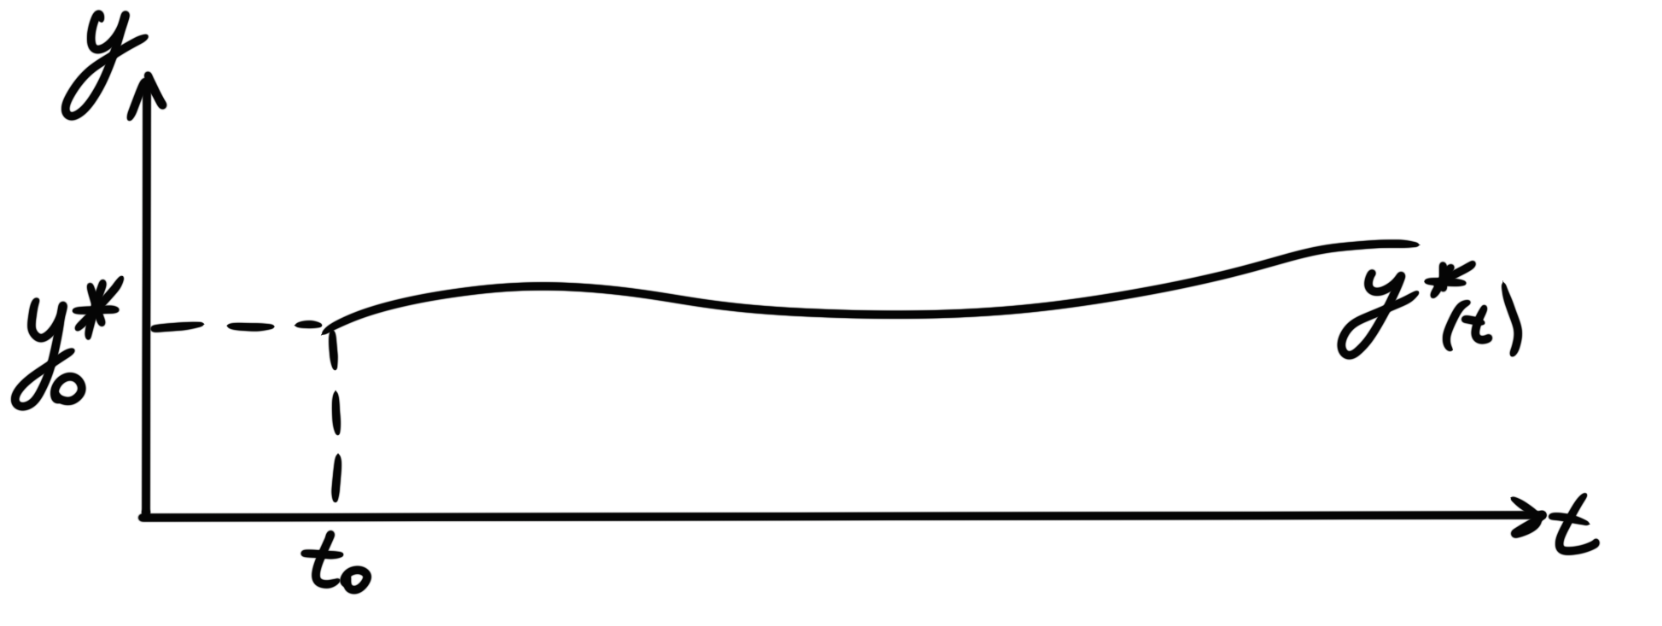
\includegraphics[width=0.3\textwidth]{/Users/vladbelousov/Desktop/Semestr_4-FP-NSU/ЭиО/Лекции_по_дням/image/31.png}
\end{center}

\[ v_{\Phi  } = \frac{\omega}{ k }  = a, \text{ }  v_g = \frac{ d \omega }{ d k}= a    \] 

2) \( \omega = \sqrt{gk } \) - волны на поверхности жидкости: 

\begin{center}
    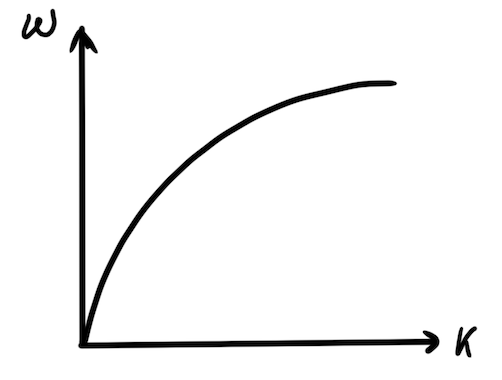
\includegraphics[width=0.3\textwidth]{/Users/vladbelousov/Desktop/Semestr_4-FP-NSU/ЭиО/Лекции_по_дням/image/32.png}
\end{center}

\[ v_{\Phi } = \sqrt{\frac{g}{k} }, \text{ }  v_g = \frac{1}{ 2} \sqrt{\frac{g}{k} } \Rightarrow v_g< v_{\Phi}     \] 

3) Электромагнитная волна в плазме: \( \omega ^2 = \omega_p ^2 + k ^2 c ^2  \) 

\begin{center}
    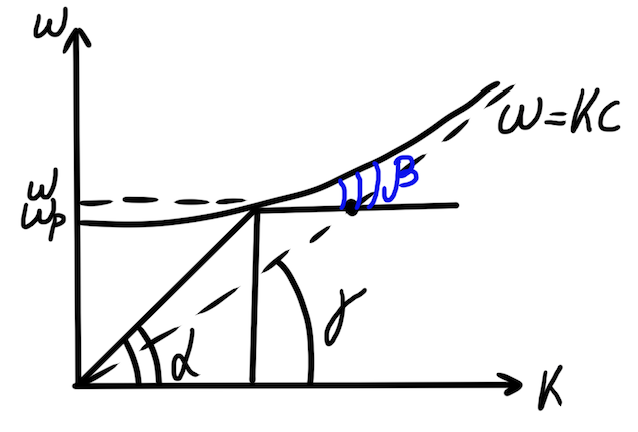
\includegraphics[width=0.3\textwidth]{/Users/vladbelousov/Desktop/Semestr_4-FP-NSU/ЭиО/Лекции_по_дням/image/33.png}
\end{center}

\[ v_{\Phi }  = \frac{\sqrt{ \omega_p ^2 + k ^2  c ^2 }}{k }, \text{ }  v_g = \frac{d \omega }{dk } =\frac{1}{2 }  \frac{2 k c ^2 }{\sqrt{ \omega_p + k ^2 c ^2 }} = \frac{ c ^2 }{v_{\Phi} } , v_g v_{\Phi }  = c ^2   \] 

\[ v_{\Phi } = tg \alpha, \text{ }  v_g = \frac{d \omega } {dk } = tg \beta , \text{ }  tg \gamma = \frac{\omega}{k }  = c   \] 

\[ \alpha > \gamma , \text{ }  \beta < \gamma \Rightarrow \alpha  > \beta - \text{ нормальная дисперсия}  :  \] 

\[ tg \alpha > tg \beta ,\quad v_{\Phi }> v_g  \] 





%%-------------------------------%%

% Закрытие документа, если файл компилируется отдельно
\ifdefined\mainfile
    % Если это основной файл, не нужно заканчивать документ
\else
    \end{document}
\fi
% Условная компиляция для самостоятельной работы
\ifdefined\mainfile
    % Если это часть основного файла, не добавляем начало и конец документа
\else
    \documentclass[12pt, a4paper]{report}
    \usepackage{/Users/vladbelousov/Desktop/Semestr_4-FP-NSU/Настройка/library}
    \usepackage[utf8]{inputenc} % Подключение поддержки UTF-8
    \begin{document}
\fi

%%-------------------------------%%

\section{Классическая теория дисперсии света в среде}

Модель взаимодействия среды с электромагнитной волной: разряженный холодный газ атомов: 

1) Частицы газа не взаимодействуют 

2) Поле, действующее на атомы, совпадают со средним полем в среде

3) Действием магнитного поля пренебрегаем 

Электроны в атоме можно приближенно разделить на: слабосвязанные (оптические), эффективно взаимодействующие с электромагнитными волнами оптического диапазона  и сильно связанные, которые слабо взаимодействуют с этими частицами 
\begin{center}
    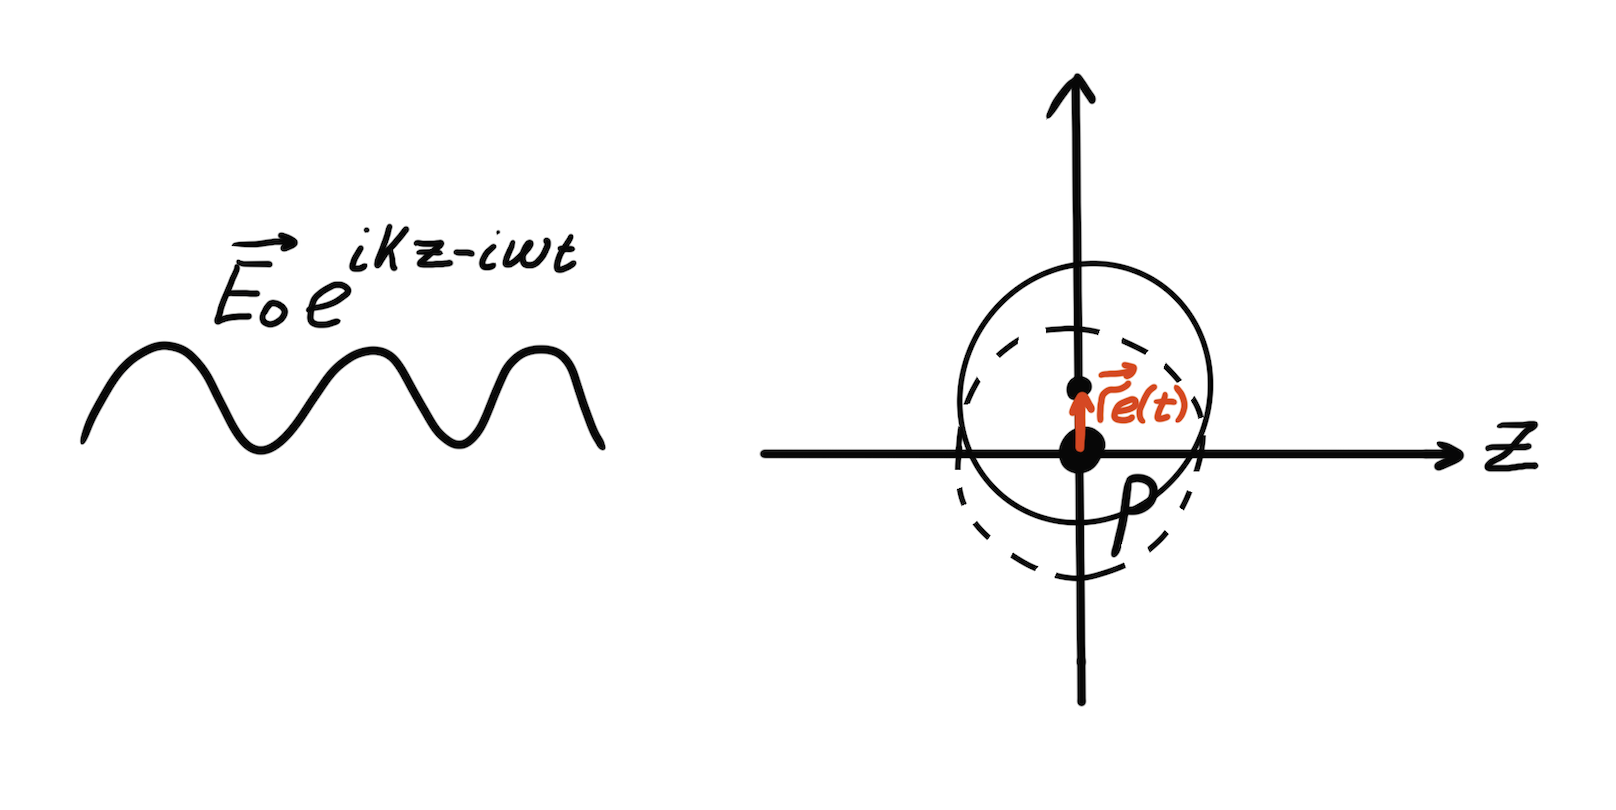
\includegraphics[width=0.6\textwidth]{/Users/vladbelousov/Desktop/Semestr_4-FP-NSU/ЭиО/Лекции_по_дням/image/34.png}
\end{center}
\[ \vec{F}_{e \to p } = \frac{4}{3 }  \pi \underbrace{\rho_e}_{ \rho = \frac{e}{\frac{4 }{3 }  \pi a ^3 } } (- \vec{r }_e (t ) )|e|   \] 

\[\Rightarrow \vec{F } _e = - \frac{e |e|}{a ^3 } \vec{r}_e (t ) = - \frac{e^2 }{a^3 } \vec{r } _e (t )      \] 

\[ \vec{F } _{p \to  e } = - \vec{ F } _{e \to  p } = - \frac{e ^2 } { a ^3 }\vec{r } _e (t )    \] 

\[ m\ddot{\vec{r}  }_e = e \vec{E }  _0 e ^{- i \omega t } - \frac{e^ 2 }{a ^3 }   \vec{r } _e(t ) +\vec{F } _{\text{трен} }    \] 

\[ \ddot{\vec{r } }_e + \underbrace{\frac{e ^2 }{m a^ 3}}_{= \omega_0 ^2 } \vec{r } _e +\underbrace{2 \gamma \dot{\vec{r } }_e}_{\frac{\text{сила трения} }{m} } = \frac{e \vec{E } _0 }{m }e^{- i \omega t }  -\text{вынужденные колебания}    \] 

\[ \vec{r        }_e  = \vec{r_0 } e^{- i \omega t }    \] 

\[ \vec{r } _{0 } ( -\omega ^2 ) + \omega_0^2 \vec{r } _0 - 2 i \gamma \omega \vec{r_0} \Rightarrow \vec{r_0 } = \frac{e \vec{E_0 } }{m } \frac{1}{\omega_0 ^2 - \omega ^2 - 2 i \gamma \omega}      \] 

\[ \vec{r_e } (t )  =\frac{e \vec{E_0 } }{m }\frac{1}{\omega_0 ^2 - \omega ^2 - 2 i \gamma \omega} e^{- i \omega t }    \] 

Далее: \( \displaystyle \vec{D }  = \vec{E }  +4 \pi \vec{P }  , \quad  \vec{P }  = n_e \vec{d }_e = n_e e \vec{r } _e (t ) \) 

\[ \vec{D }  = \vec{E }  _0 e^{ -i \omega t } + 4 \pi n_e \frac{e \vec{E } _0 }{m } \frac{1}{\omega_0 ^2 - \omega ^2 - 2 i \gamma \omega} e^{- i \omega t }  = \underbrace{\left(  1+ \overbrace{\frac{4 \pi n_e e ^2 } { m }}^{\omega_p ^2 } \frac{1}{\omega_0 ^2 - \omega ^2 -  2 i \gamma \omega  }\right) }_{\varepsilon ( \omega)}\underbrace{\vec{E }  _0 e^{- i \omega t }}_{\vec{E }(t ) }     \] 

1 случай: Дисперсия вдали от линии поглощения 

\[ |\omega_0 ^2 - \omega ^2 | \gg 2 \gamma \omega  \] 

Уравнение дисперсионное соотношение: \( \displaystyle \frac{\omega \sqrt{\varepsilon ( \omega )\mu ( \omega )}}{c } = k , \mu (\omega ) = 1   \) 

\[ \varepsilon (\omega ) \simeq 1+ \frac{\omega_p ^2 } { \omega_0 ^2 - \omega ^2 } \Rightarrow n ( \omega ) \simeq \sqrt{\varepsilon (\omega )} \simeq 1+ \frac{\omega_p ^2 } {2(\omega_0 ^2 - \omega ^2) }       \] 

\begin{center}
    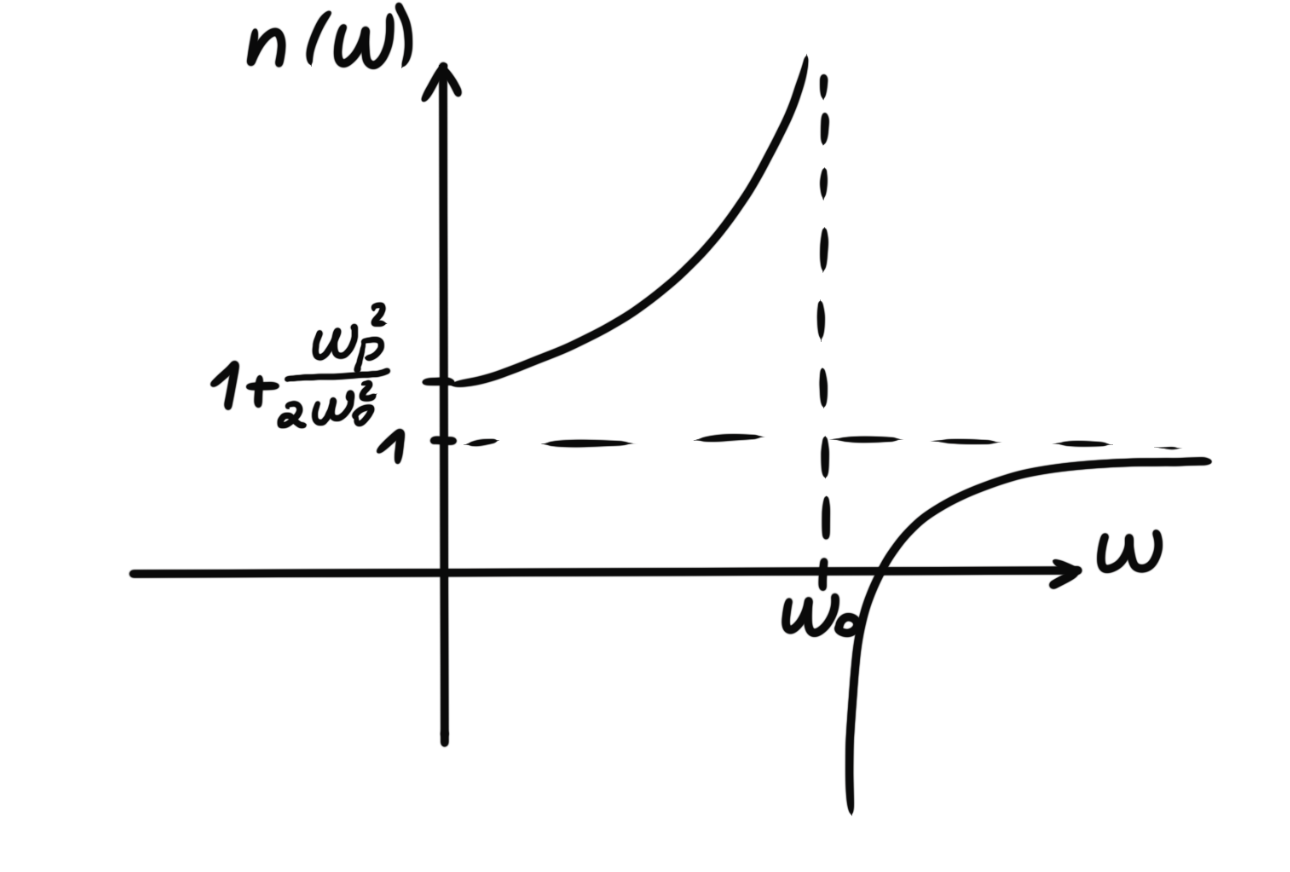
\includegraphics[width=0.6\textwidth]{/Users/vladbelousov/Desktop/Semestr_4-FP-NSU/ЭиО/Лекции_по_дням/image/35.png}
\end{center}

\[ \frac{dn ( \omega)}{d \omega} > 0 - \text{ нормальная дисперсия }: v_{g } < v_{\Phi }     \] 

2 случай: Дисперсия вблизи линии поглощения \( \omega \simeq \omega_0  \) 

\[ \omega = \omega_0 \Delta \omega , \quad  \Delta \omega \ll \Rightarrow \omega_0 ^2 - ( \omega+ \Delta \omega ) ^2 - 2 i \gamma ( \omega_0 + \Delta \omega ) = -2 \omega_0 \Delta \omega - \Delta \omega ^2 - 2 i \gamma \omega_0 - 2 i \gamma \Delta\omega   \] 

\[ \varepsilon ( \omega ) \simeq 1 - \frac{ \omega_p ^2 }{2 \omega_0 (\Delta \omega + i \gamma)}; \quad  n( \omega ) = \sqrt{\varepsilon( \omega)} \simeq 1 \frac{ \omega_p ^2 }{4 \omega_0 (\Delta \omega + i \gamma)} \frac{ \Delta \omega - i \gamma }{\Delta \omega - i \gamma} =     \] 

\[ =1  -\frac{\omega_p ^2 \Delta \omega}{4 \omega_0 (\Delta \omega ^2 + \gamma ^2)} + i \frac{ \omega_p ^2 \gamma }{4 \omega_0(\Delta \omega ^2 + \gamma ^2) }= 1- \frac{ \omega_p ^2 }{4 \omega_0 \gamma }\frac{ ( \frac{\Delta \omega}{\gamma} )}{1+ \left( \frac{\Delta \omega}{\gamma}  \right) ^2 } + i \frac{\omega_p ^2 }{4 \omega_0\gamma } \frac{ 1}{1+ \left( \frac{\Delta \omega}{\gamma}  \right) ^2}    \] 

\begin{center}
    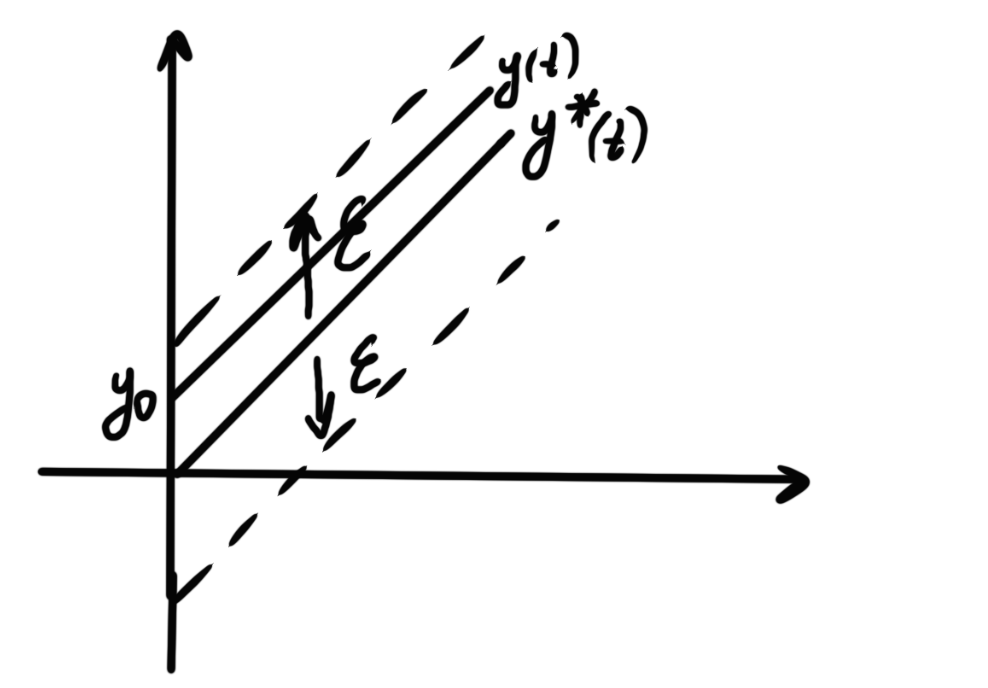
\includegraphics[width=0.45\textwidth]{/Users/vladbelousov/Desktop/Semestr_4-FP-NSU/ЭиО/Лекции_по_дням/image/36.png}
    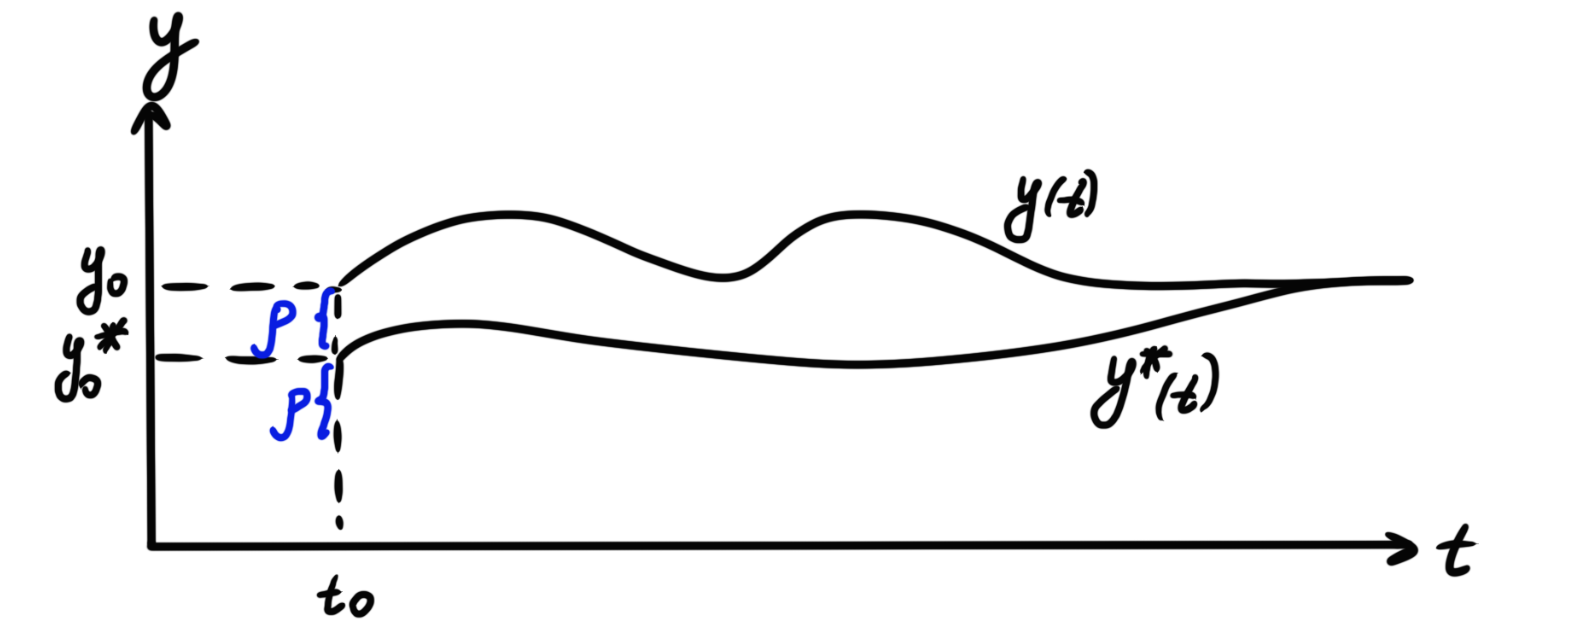
\includegraphics[width=0.45\textwidth]{/Users/vladbelousov/Desktop/Semestr_4-FP-NSU/ЭиО/Лекции_по_дням/image/37.png}
\end{center}

\[ k = \frac{\omega}{c }  \sqrt{ \varepsilon ( \omega )} = \frac{ \omega n ( \omega )}{c }  = \frac{\omega}{ c } \mathrm{Re } (n (\omega))+ \frac{i \omega}{c } \mathrm{Im }  (n (\omega))    \] 

\begin{center}
    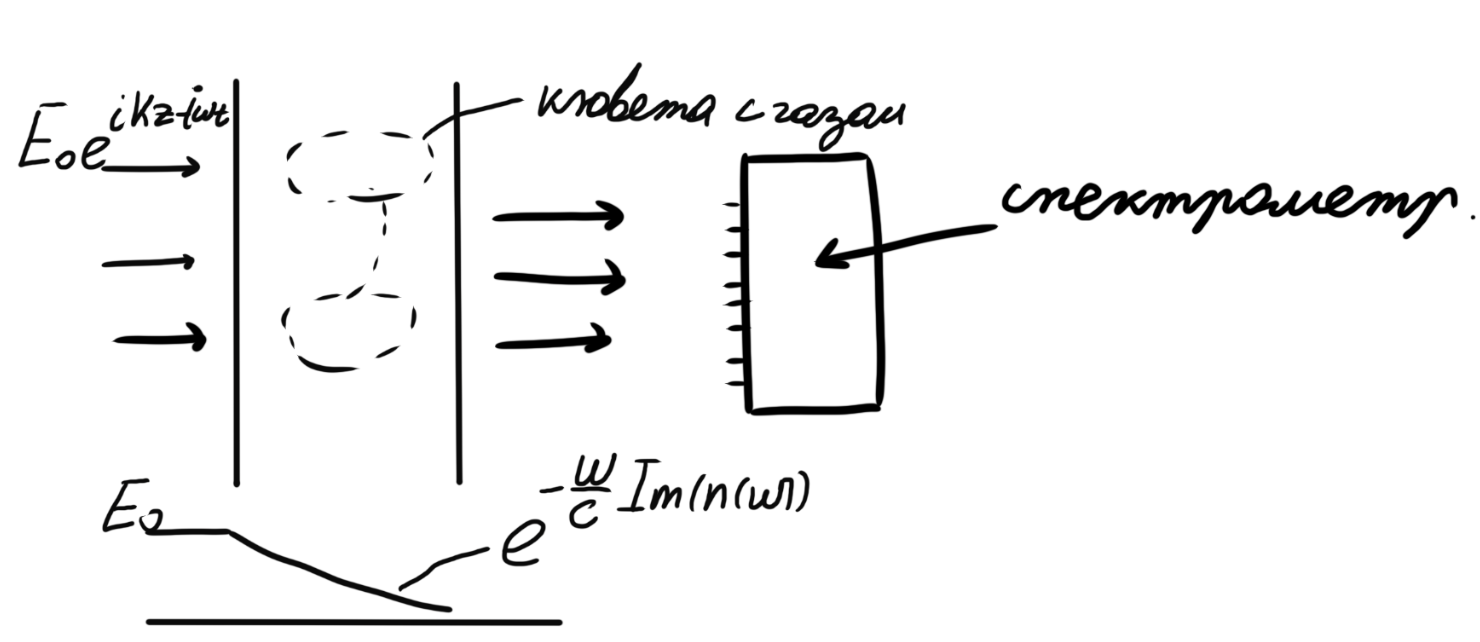
\includegraphics[width=0.6\textwidth]{/Users/vladbelousov/Desktop/Semestr_4-FP-NSU/ЭиО/Лекции_по_дням/image/38.png}
\end{center}

\[ \vec{E } (z, t ) = \vec{E } _ 0 e ^{ i \frac{\omega}{c } \mathrm{Re } (n ( \omega )) - i \omega t  } e^{- \frac{\omega}{ c } \mathrm{Im } (n ( \omega )) z  } \] 

Показания спектрометра: 

\begin{center}
    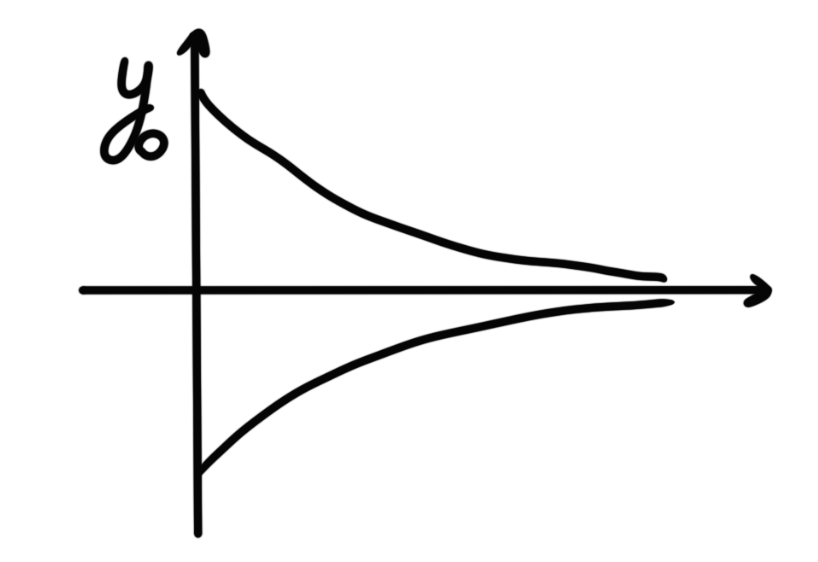
\includegraphics[width=0.6\textwidth]{/Users/vladbelousov/Desktop/Semestr_4-FP-NSU/ЭиО/Лекции_по_дням/image/39.png}
\end{center}

В квантовой теории \(\displaystyle  \varepsilon ( \omega ) = 1 + \frac{3 \pi Na e ^2 }{m } \sum_{n=1}^{\infty  } \frac{f_n }{\omega_{on } ^2 - \omega ^2 -2 i \gamma_n \omega }    \) 

\begin{center}
    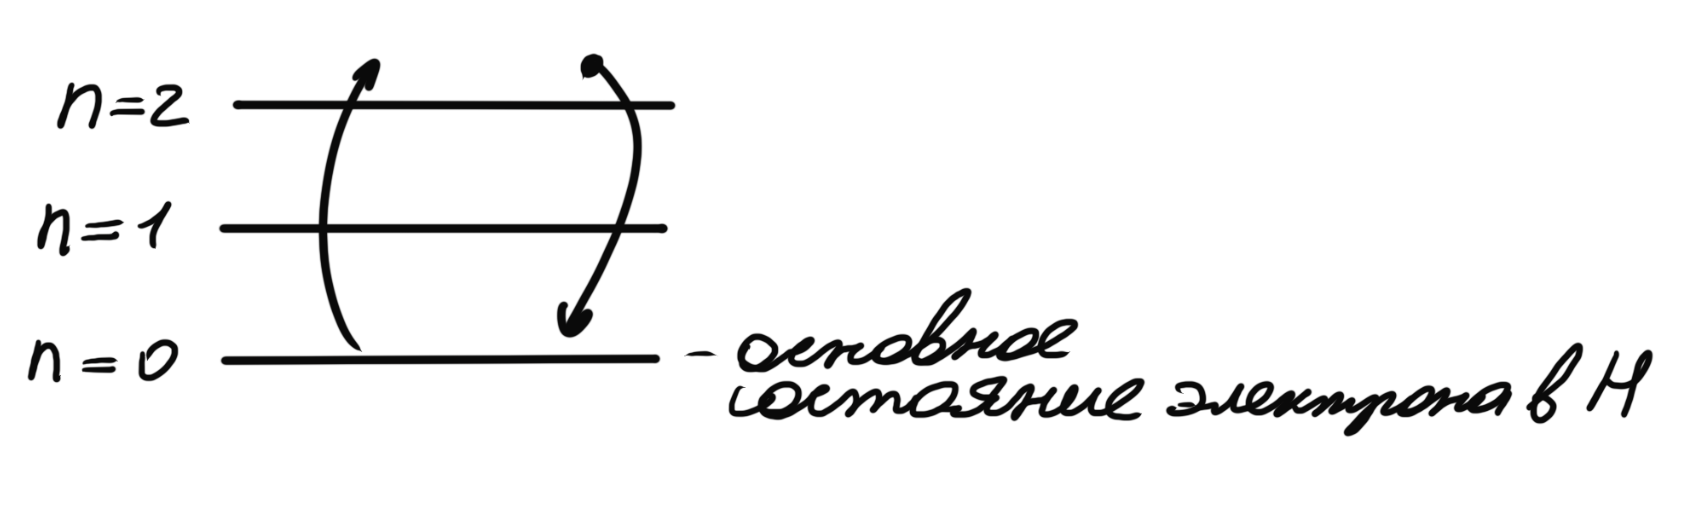
\includegraphics[width=0.6\textwidth]{/Users/vladbelousov/Desktop/Semestr_4-FP-NSU/ЭиО/Лекции_по_дням/image/40.png}
\end{center}

\[ h \omega _{on     } = \varepsilon_n -\varepsilon_0 - \text{энергия перехода с n-го уровня на основной} ,\quad  h = 1,054 \cdot 10 ^{-27} \text{эрг с }    \]  

\[ f_n - \text{сила осциллятора - вероятность перехода с n-го уровня на основной  } \Rightarrow \sum_{n =1} ^{\infty  } f_n = 1   \] 

\section{ Стоячие волны}

\begin{center}
    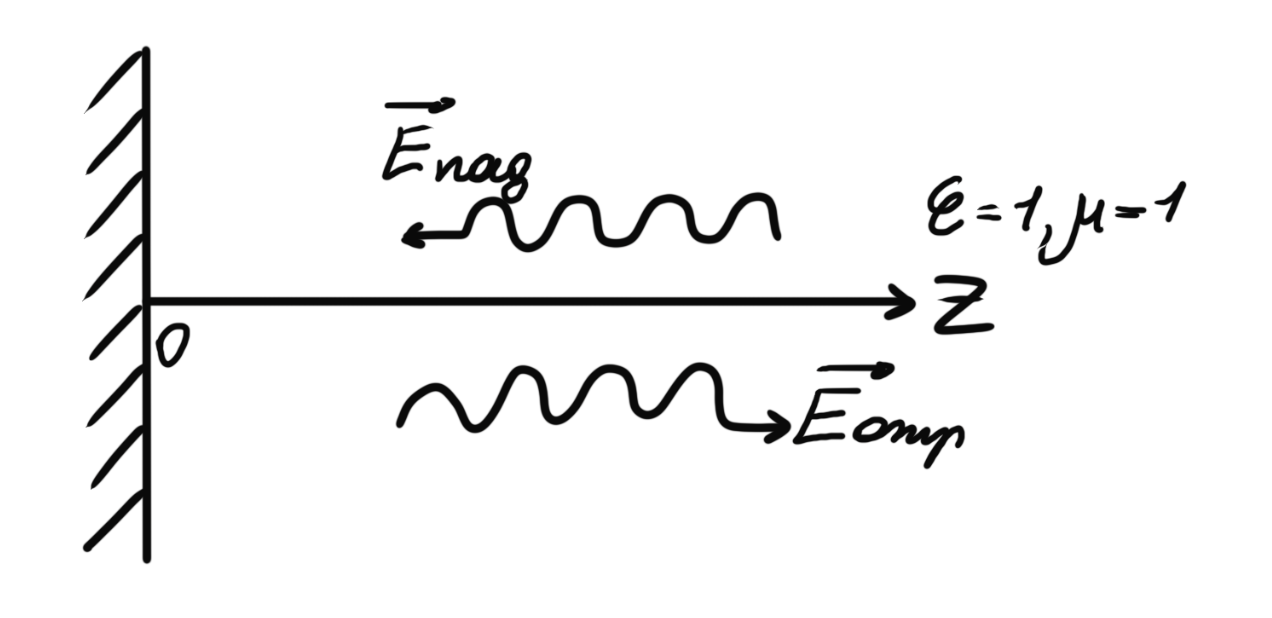
\includegraphics[width=0.6\textwidth]{/Users/vladbelousov/Desktop/Semestr_4-FP-NSU/ЭиО/Лекции_по_дням/image/41.png}
\end{center}

\[ \vec{E } _{\text{пад } } =   \vec{E }  _ 0 e^{i (\vec{k},\vec{r }     )- i \omega t }  = \vec{E } _0 e^{- i k z - i \omega t } \quad ( \vec{E } _0 \perp \vec{n }  = - \vec{e } _z ), \quad \vec{k } = \vec{n } k = - \vec{e }_z k\] 

\[ \vec{E } _{\text{отр }  } = \vec{E } _1 e^{i kz - i \omega t }, \quad  \vec{E } _1 \perp \vec{e }_z     \] 

Граничные условия на поверхности проводника

\[ \vec{E } , \vec{\tau }_{\text{Г } } = 0 , \quad E_{\tau } =( \vec{E } _ 0 ,\vec{\tau } )+ ( \vec{E } _ 1 , \vec{\tau } ) = 0 = ((\vec{E } _0 + \vec{E } _1), \vec{\tau } )= 0      \] 

\[ \Rightarrow \vec{E_0} + \vec{E_1 } = 0 \Rightarrow \vec{E_0 } = -\vec{E_1}      \] 

\[ \vec{E}_{\Sigma } = \vec{E_0 }e^{ - i kz - i\omega t}  - \vec{E_0 }e^{i kz - i \omega t } = \vec{E_0 }e^{- i \omega t } \frac{ e^{- ikz } - e^{i kz } }{2i } 2 i= -2i \vec{E_0 }\sin (kz) e^{- i \omega t }          \] 

\[ \vec{B }  = \vec{H }  = \sqrt{\frac{ \varepsilon }{\mu } } [ \vec{n } \times  \vec{E } ]  \]

\[ \vec{B }_{\text{пад } } = [ - \vec{e } _z \times  \vec{E_0}  ]   e^{- ikz - i \omega t } , \quad  \vec{B }_{\text{отр } } = [  \vec{e } _z \times  (-\vec{E_1 }) ] e^{ikz - i \omega t } \] 

1 пример: падающая волна линейно поляризована 

\[ \vec{E_0 } = \vec{e_x  }|c_1         | e^{i \varphi } , \text{ }  c_1 \in \mathbb{C} ; \text{ } \mathrm{Re }  (\vec{E }_{\Sigma }( z, t ))  = - 2 |c_1 | \vec{e } _x \sin(kz ) \sin (\omega t  - \varphi )        \] 

\[ \mathrm{Re } (\vec{B } _{\Sigma } (z, t ) ) = - 2 \vec{e }  _{y }  \cos ( kz ) \cos  ( \omega t - \varphi ) |c_1 | \] 

\begin{center}
    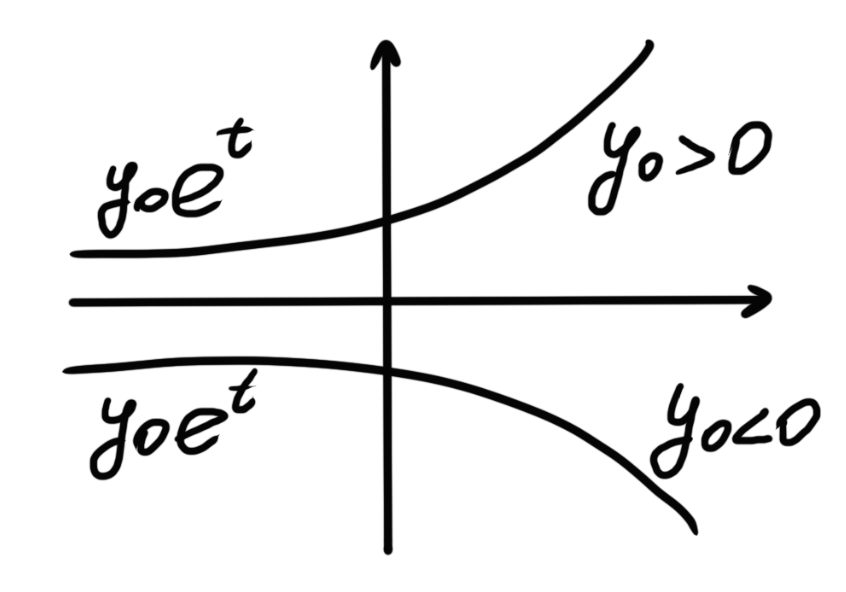
\includegraphics[width=0.6\textwidth]{/Users/vladbelousov/Desktop/Semestr_4-FP-NSU/ЭиО/Лекции_по_дням/image/42.png}
\end{center}
Узлы: \( k z_{m }= m \pi , z_{m }  = \frac{m \lambda }{2 } \) 


Пучность: \( k z_{m } ' = m \pi + \frac{\pi}{2 } , \quad  z_m ' = \frac{ m \pi + \frac{\pi}{2} }{k } = \frac{m \lambda }{2} + \frac{\lambda}{ 4 }    \) 

2 пример: круговая поляризация \( \vec{E } _0 = ( \vec{e } _ x + i \vec{e } _ y ) |c_1 |e^{ i \varphi} - \text{левая круговая}  \) 

\[ \mathrm{Re } (\vec{E } _{\Sigma }(z, t ) ) = \mathrm{Re }  \left[ -2 i ( \vec{e } _ x + i \vec{e }  _ y )|c_1|e^{- i ( \omega t - \varphi )} \sin (kz)  \right]= -2 |c_1 | \sin (kz) [\vec{e } _ x \sin (\omega t - \varphi) - \vec{e } _y \cos (\omega t - \varphi )]  \] 

\[ \mathrm{Re } (\vec{B }_{\Sigma }( z, t )  ) =2 |c_1 | \cos (kz) [\vec{e } _ x \sin (\omega t - \varphi) - \vec{e } _y \cos (\omega t - \varphi )]   \] 

%%-------------------------------%%

% Закрытие документа, если файл компилируется отдельно
\ifdefined\mainfile
    % Если это основной файл, не нужно заканчивать документ
\else
    \end{document}
\fi
% Условная компиляция для самостоятельной работы
\ifdefined\mainfile
    % Если это часть основного файла, не добавляем начало и конец документа
\else
    \documentclass[12pt, a4paper]{report}
    \usepackage{/Users/vladbelousov/Desktop/Semestr_4-FP-NSU/Настройка/library}
    \usepackage[utf8]{inputenc} % Подключение поддержки UTF-8
    \begin{document}
\fi

%%-------------------------------%%

Пусть \(\displaystyle  0 < kz < \frac{\pi}{4}   \Rightarrow 0 < \sin (kz ) < \cos (kz ) < 1 \) 

\begin{center}
    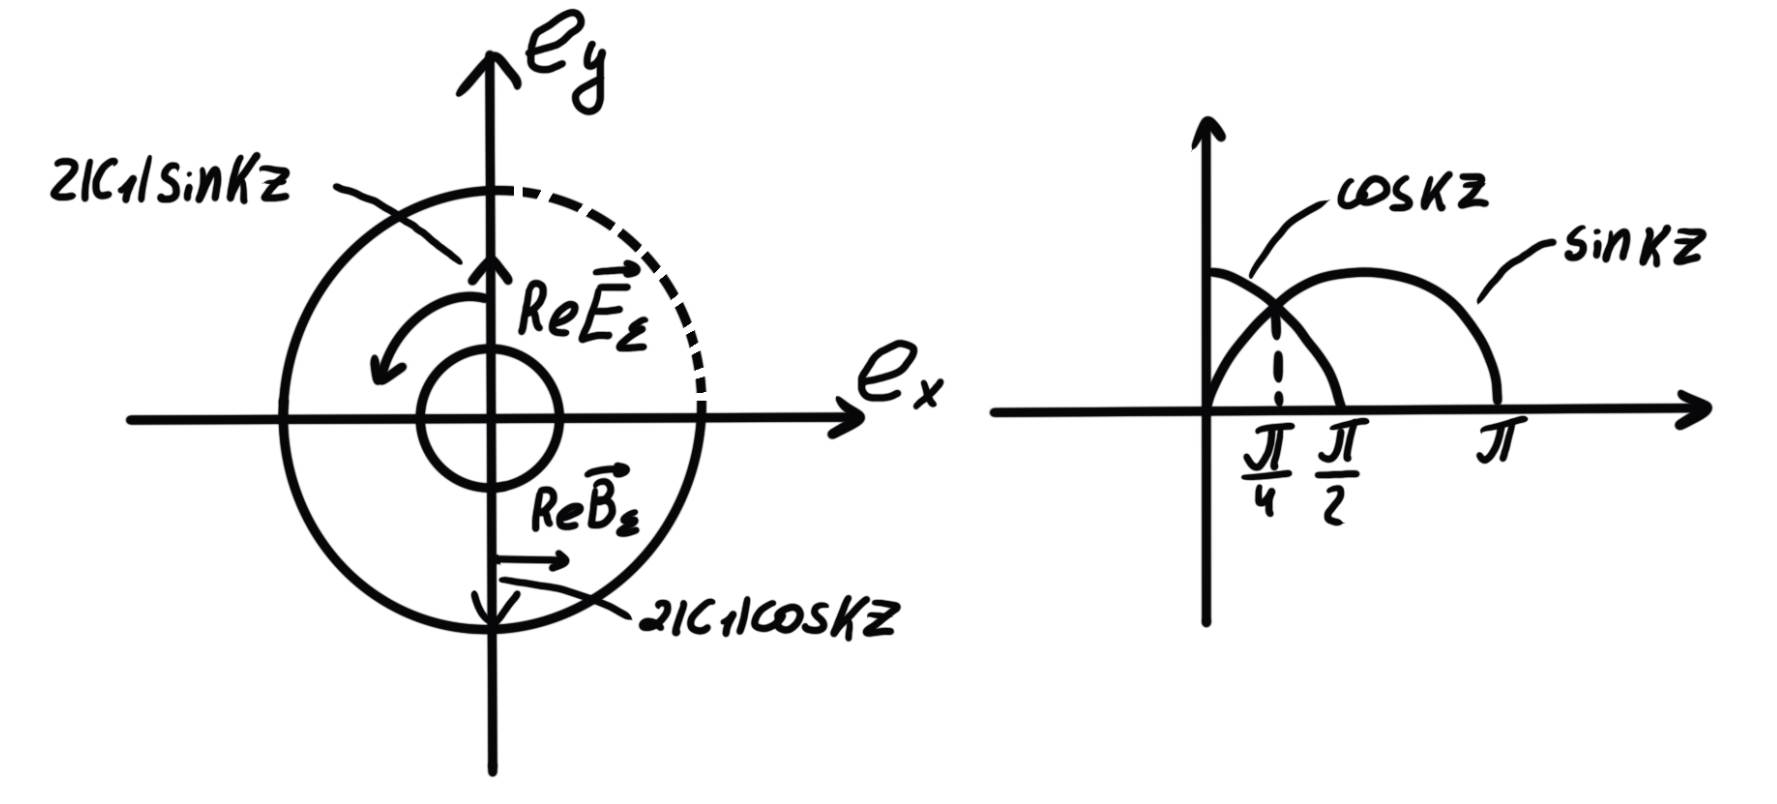
\includegraphics[width=0.6\textwidth]{/Users/vladbelousov/Desktop/Semestr_4-FP-NSU/ЭиО/Лекции_по_дням/image/43.png}
\end{center}

\section{Резонаторы}

- полость, окруженная идеальным проводником. 

В нем накапливаются волны собственной волны резонатора. Таким образом резонатор фильтрует сигнал по определенной частоте и усиливает его сингал. С помощью резонаторов можно ускорять сгустки протонов и электронов.


Способы возбуждения резонаторов: 

1) Штырь с переменным во времени потенциалом. 

2) Петля с переменным током. 

3) Модулированный электронный пучок. 

4) Волновод с бегущей волной. 

Уравнения электромагнитных полей в резонаторе:

\[ \vec{ E } (\vec{r } , t ) = \vec{E_0  }(\vec{r } ) e^{ - i \omega t }   \] 

\[ \vec{B }  (\vec{r } , t )    = \vec{B_0 }(\vec{r } ) e^{ - i \omega t }  \] 

Из уравнений Максвелла следует, что:

\[ \mathrm{rot } \vec{E_0 }(\vec{r } ) e ^{ -i\omega t } = -\frac{i \omega }{c } \vec{B_0 }(\vec{r } ) e^{ -i \omega t}  \Rightarrow \mathrm{div } \vec{B_0 } = 0        \] 

\[ \mathrm{rot } \vec{H_0 }(\vec{r }  ) = - \frac{i \omega }{c } \vec{D_0 }(\vec{r} )  \Rightarrow  \mathrm{div } \vec{D_0  } = 0      \] 

Если внутри резонатора вещество с \( \varepsilon ( \omega ) \) и \( \mu ( \omega ) \Rightarrow \vec{B_0 } = \vec{H_0 } \mu(\omega) ,\text{ }  \vec{D_0 } = \vec{E_0 } \varepsilon ( \omega )   \)   

Граничные условия: 

\[ E_{0 \tau} |_{\text{Г } }  = 0, \quad  B_{0 n} |_{\text{Г } }  = 0  \] 

\begin{center}
    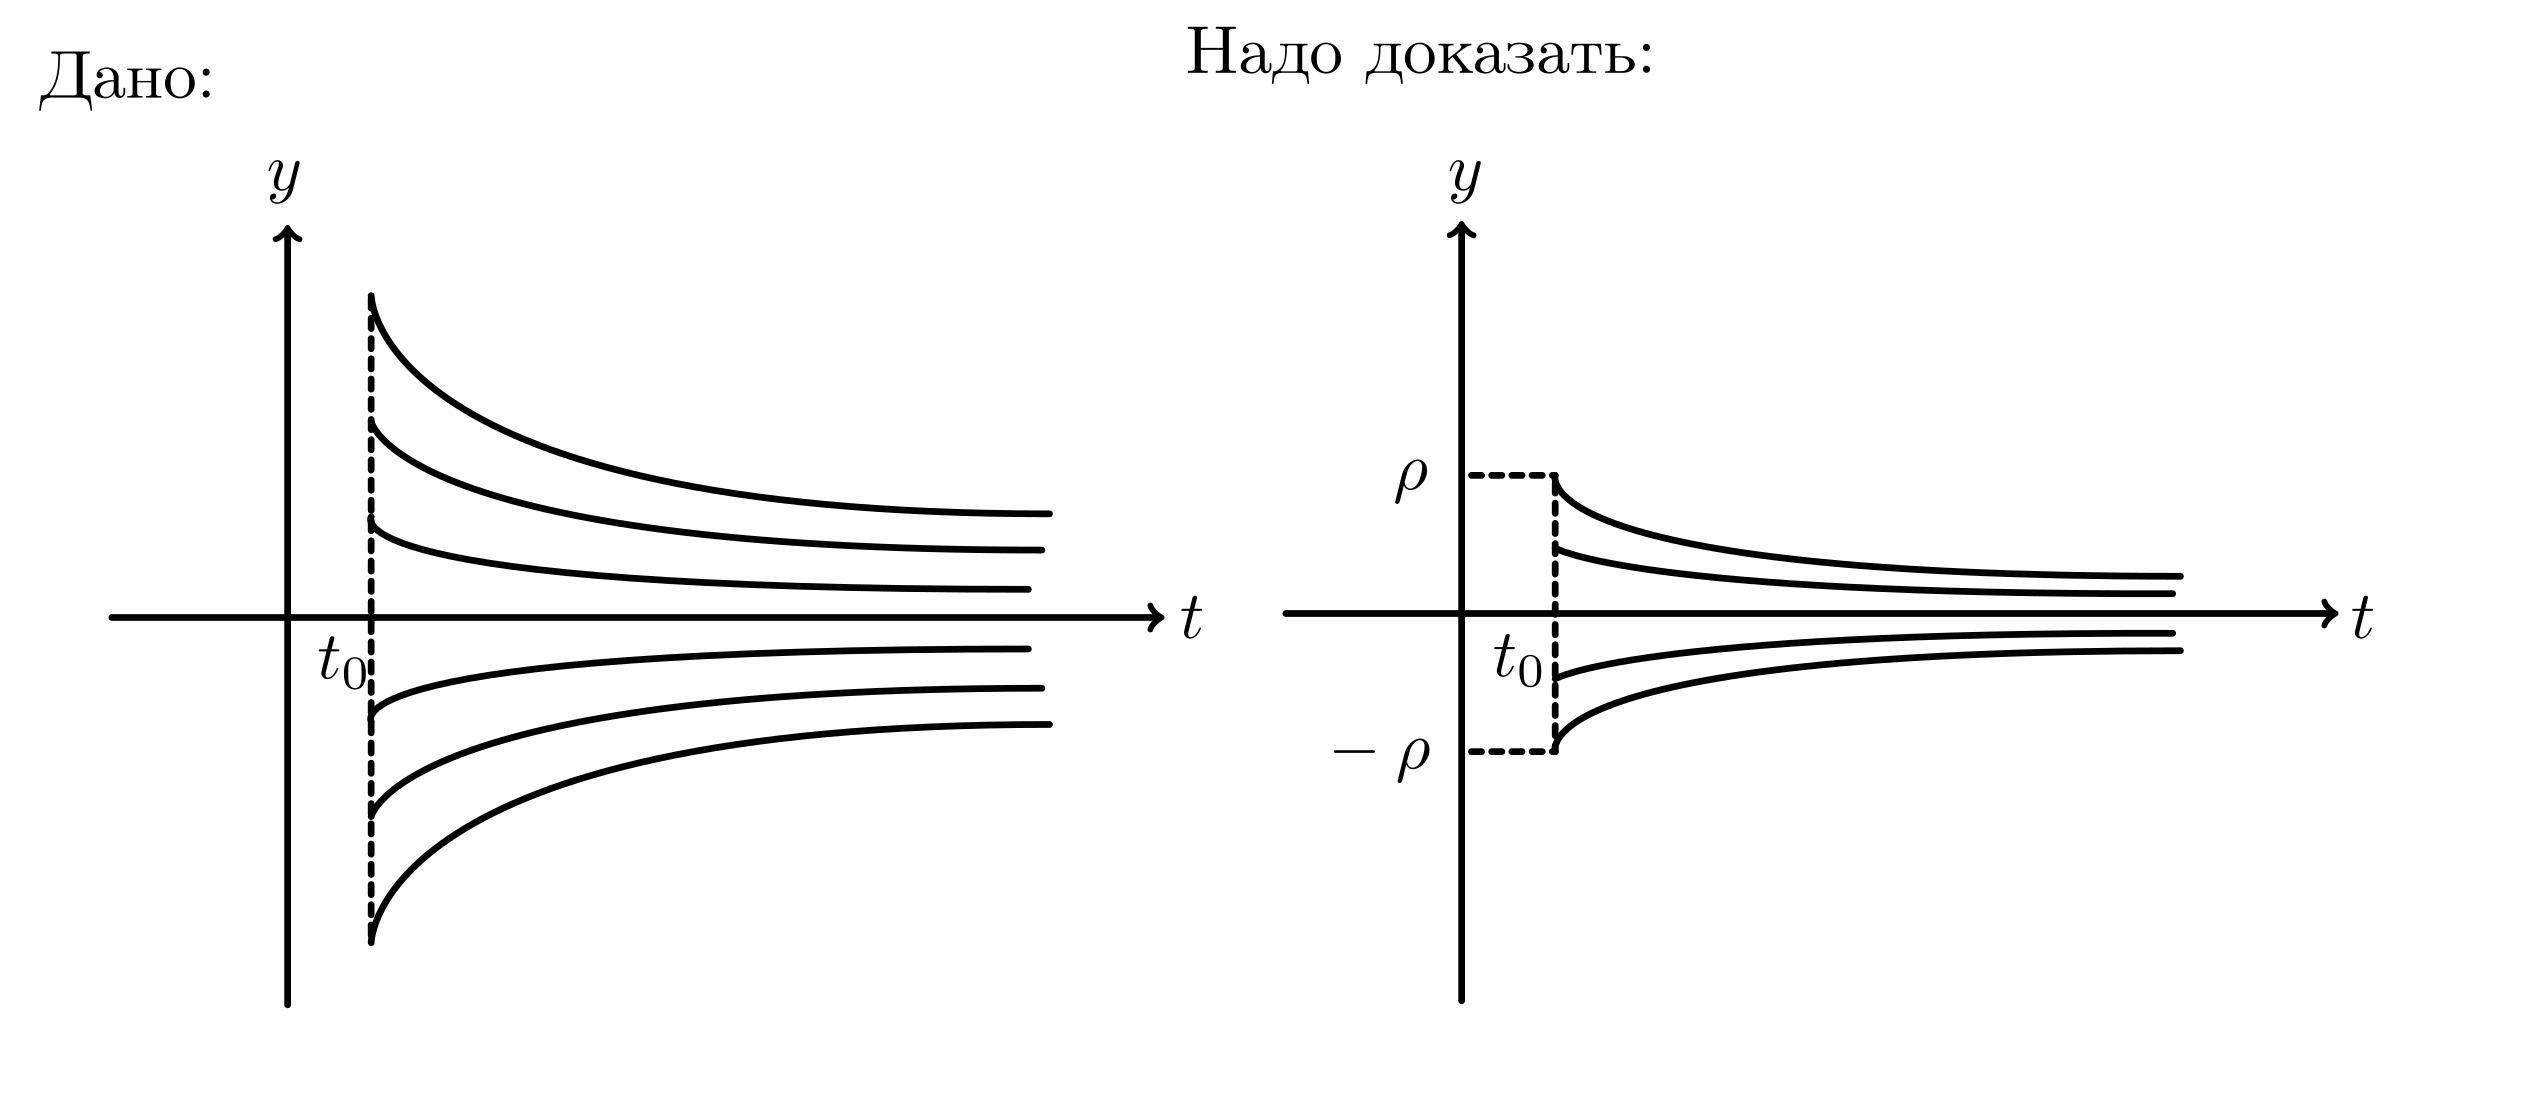
\includegraphics[width=0.2\textwidth]{/Users/vladbelousov/Desktop/Semestr_4-FP-NSU/ЭиО/Лекции_по_дням/image/44.png}
\end{center}

%картинка для пояснения направлений из РУслана 



\[ \begin{aligned}
    \begin{array}{l|}
        \displaystyle (\mathrm{rot }  \vec{E_0})_z =  + \frac{i \omega }{c } B_{0z}   \\
        (\mathrm{rot }  \vec{E_0})_z = \underbrace{\frac{\partial E_{0y } }{\partial  x}}_{=0} - \underbrace{\frac{\partial  E_{0x } }{\partial  y } }_{=0}  \\
        E_{0y } |_{\text{Г} } =0 , \text{ }  E_{0x } |_{\text{Г} } =0 
    \end{array}
    \Rightarrow  B_{0z } = 0
\end{aligned} \] 

Исключим \( \vec{B_0 } (\vec{r } ) \) из уравнений: 

\[ \mathrm{rot } \mathrm{rot } \vec{E_0 }( \vec{r }  ) = \underbrace{\nabla \mathrm{div } \vec{E_0 }(\vec{r } )}_{\frac{\mathrm{div } \vec{D_0 }(\vec{r } )}  {\varepsilon(\omega)} = 0} - \Delta \vec{E_0 } (\vec{r } )  = \frac{i \omega }{c} \mu (\omega )\left( -\frac{ i \omega}{c}  \right) \varepsilon(\omega ) \vec{E_0 }(\vec{r } )   \Rightarrow   \] 

\[  \Rightarrow \begin{aligned}
    \begin{cases}
        \displaystyle \Delta \vec{E_0 }(\vec{r } ) + \frac{ \omega ^2 }{c ^2 }\varepsilon( \omega ) \mu (\omega ) \vec{E_0 }(\vec{r } ) = 0 \\
        \displaystyle \mathrm{div } \vec{E_0 }(\vec{r } ) = 0 
    \end{cases} 
    + \text{Г.У: } E_{0 \tau} |_{\text{Г } }  = 0 
\end{aligned}  \] 

\[ \frac{ \omega ^2 }{c ^2 }\varepsilon( \omega ) \mu (\omega ) = k ^2  \] 

- эта система является краевой трех мерной задачей Штурмана-Лиувиля.

\textbf{Задача Штурма-Лиувиля}: 

1) Решение \( \exists    \)  только для бесконечного ряда чисел \( k_n \) - собственные числа; 

2) Каждому \( k_n \) соответствует как минимум одна собственная функция -  собственное колебание;

3) Набор всех собственных  функций образует фундаментальную систему ортогональных функций, по которым можно разложить поля внешнего источника возбуждения. 

4) \(\displaystyle  \min (k_n ) \sim \frac{1}{l}  \Rightarrow \varepsilon = 1, \text{ }  \mu =1 , \text{ }\omega _{\min  } \sim \frac{c}{l}     \) 

Примеры резонаторов: 

1) Плоский резонатора

\begin{center}
    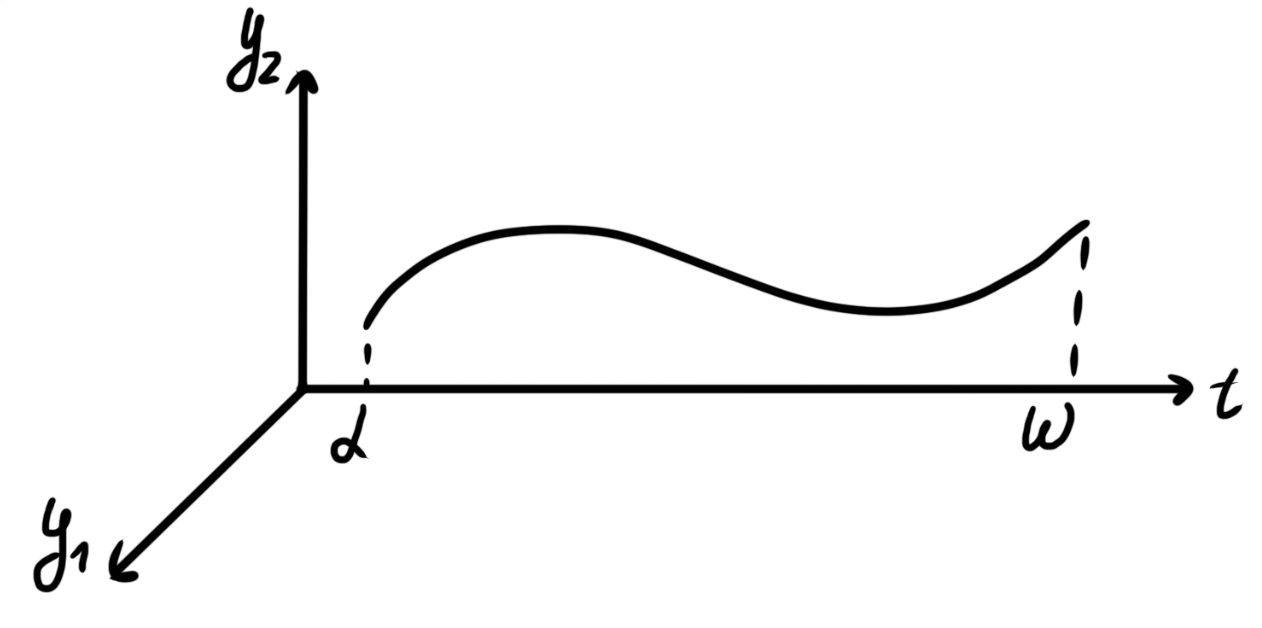
\includegraphics[width=0.3\textwidth]{/Users/vladbelousov/Desktop/Semestr_4-FP-NSU/ЭиО/Лекции_по_дням/image/45.png}
\end{center}

Решение как в задаче про отражение: \( \displaystyle  \vec{E } _{\Sigma} ( \vec{r } , t ) = -2 i \vec{E_0} \sin (kz ) e^{ - i \omega t }  \) 

\[ \Rightarrow \sin (kL ) = 0 \Rightarrow k_m L = m \pi \Rightarrow k_m = \frac{m \pi }{L}   - \text{собственные числа}  \] 

\[ k_{\min  } = \frac{\pi}{ L }  , \text{ } \omega_{ \min } (\varepsilon = 1, \text{ }  \mu =1 )  = \frac{ \pi c }{L}   \] 

\begin{center}
    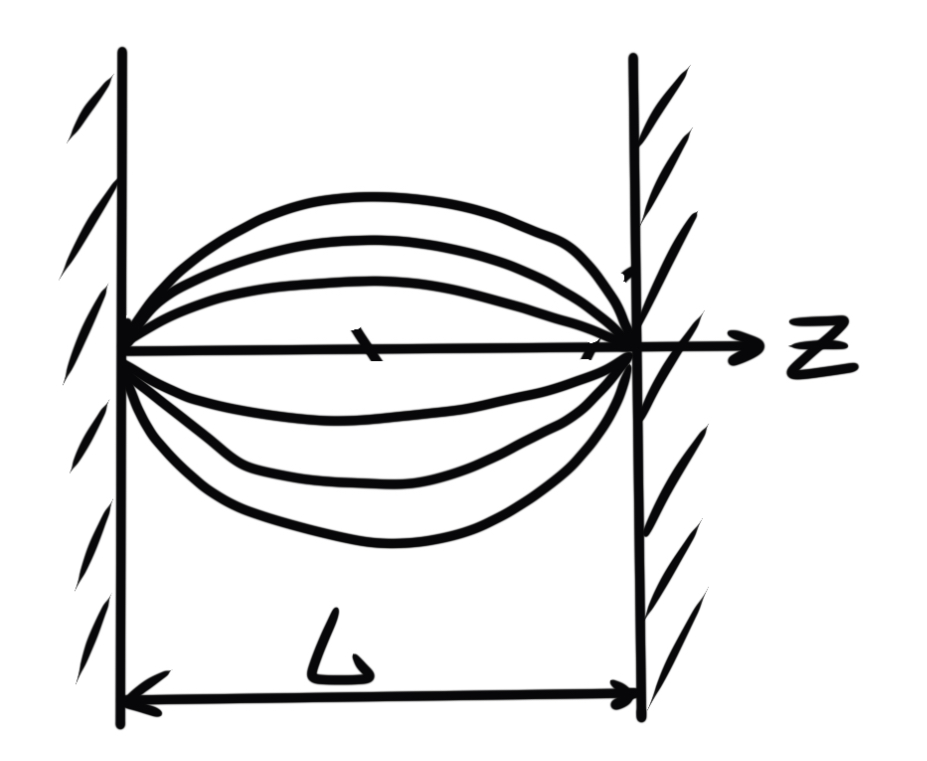
\includegraphics[width=0.3\textwidth]{/Users/vladbelousov/Desktop/Semestr_4-FP-NSU/ЭиО/Лекции_по_дням/image/46.png}
\end{center}

2) Прямоугольный трех мерный резонатор: 

\begin{center}
    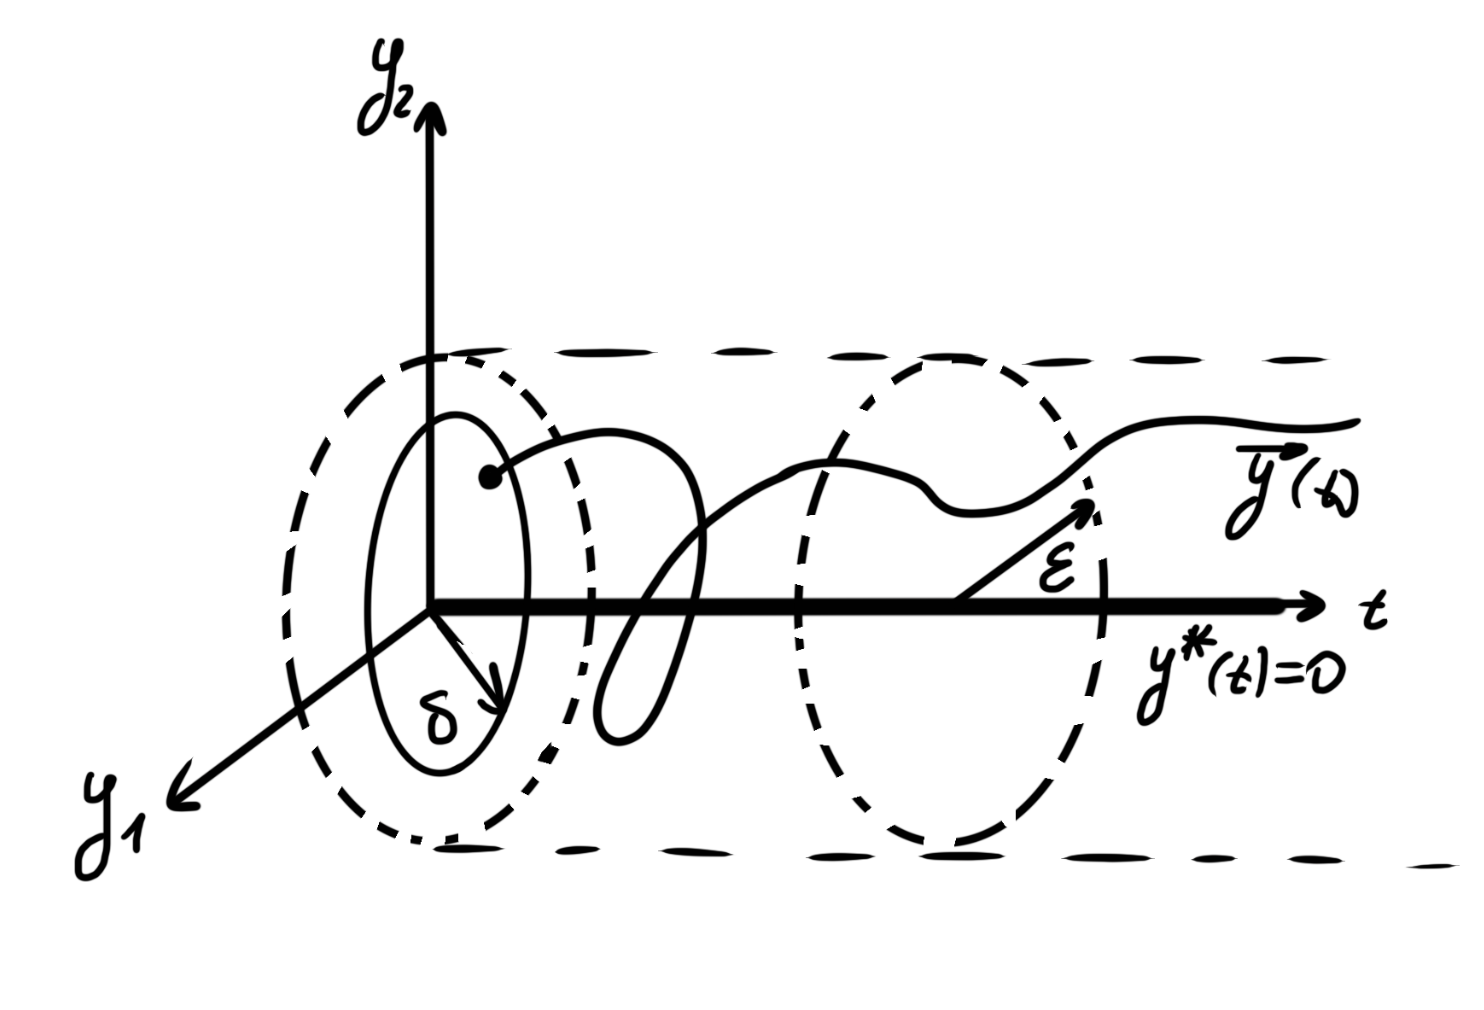
\includegraphics[width=0.4\textwidth]{/Users/vladbelousov/Desktop/Semestr_4-FP-NSU/ЭиО/Лекции_по_дням/image/47.png}
\end{center}

\[ \Delta \vec{E_0 }(\vec{r } )  + k ^2 \vec{E_0 }(\vec{r } ) = 0 , \text{ }  \mathrm{div } \vec{E_0 }(\vec{r } ) = 0 , \text{ } E_{0 \tau} |_{\text{Г } }  = 0   \] 

\[ \left( \frac{\partial  ^2 }{\partial  x ^2 } + \frac{\partial  ^2 }{ \partial  y ^2 } + \frac{\partial  ^2 }{\partial  z ^2 }    \right) \begin{pmatrix}
    E_{0x}\\
    E_{0y} \\
    E_{0z} 
    \end{pmatrix} + k ^2 \begin{pmatrix}
        E_{0x}\\
        E_{0y} \\
        E_{0z} 
    \end{pmatrix} = 0\] 

Пусть \( E_{0x } (\vec{r } )    = E_1 (x) E_2 (y) E_3 (z) \) 

\[ E_2( y )E_3 ( z ) \frac{d ^2 E_1 ( x ) }{dx ^2 } + E_1 ( x ) E_3 ( z ) \frac{d ^2 E_2 ( y ) }{dy ^2 } + E_1 ( x ) E_2 ( y ) \frac{d ^2 E_3 ( z ) }{dz ^2 } + k ^2 E_1 ( x ) E_2 ( y ) E_3 ( z ) = 0 | : E_1 E_2 E_3   \] 

Двигаясь вдоль \( x \)  все члены кроме \( \displaystyle \frac{E_1 ''(x)}{E_1 (x)}  \), точно константы значит используя следующее выражение:  

\[ \frac{E_1 '' ( x )}{E_1(x) } + \frac{E_2 '' ( y )}{E_2(y) } + \frac{E_3 '' ( z )}{E_3(z) } + k ^2 = 0  \text{ , получаем: }  \frac{E_1 ''( x )}{ E_1( x )} = \mathrm{const} ; \underbrace{\text{ } \frac{E_2 ''( y )}{ E_2( y )} = \mathrm{const} , \text{ } \frac{E_3 ''( z )}{ E_3( z )} = \mathrm{const} }_{\text{Аналогочино} }.    \] 

\[ E '' ( x ) = \alpha E (x  ) \quad  \text{ Решение ищем в виде: } E_1(x ) = c_1 e^{\lambda x} \Rightarrow c_1 \lambda ^2 e^{\lambda x } = \alpha c_1e^{\lambda x } \Rightarrow \lambda_{1,2 }  = \pm \sqrt{\alpha }       \] 

\( 1.\text{ }  \alpha > 0 \Rightarrow E (x )  = A e^{ \sqrt{\lambda} x }+ B e^{- \sqrt{\lambda} x }   \) занулить решение на двух стенках \( x=0 , \text{ }  x= a \) -  невозможно 

\( 2.\text{ } \alpha = 0 \Rightarrow E (x ) =  A x + B     \) - аналогично невозможно

\( 3. \text{ }  \alpha < 0 \Rightarrow E ( x )  = A e^{+ i\sqrt{\left\lvert \alpha \right\rvert}x} + B e^{- i\sqrt{\left\lvert \alpha \right\rvert}x}  = c_1 \sin ( \sqrt{\left\lvert \alpha \right\rvert}x + \varphi )  \) - имеет периодически нули, что может удовлетворять границам

Переобозначение: \(\alpha_x = - k ^2 _x , \alpha_y = - k ^2 _y , \alpha_z = - k ^2 _z  \) 

\[ E_{0x}  ( \vec{r } ) = A \sin (k_x x + \alpha_x) \sin (k_y y + \alpha_y) \sin (k_z z + \alpha_z), \alpha_x, \alpha_y, \alpha_z = \mathrm{const} \] 

\[ E_{0y} = B \sin (k_x x + \beta_x) \sin (k_y y + \beta_y) \sin (k_z z + \beta_z), \beta_x, \beta_y, \beta_z = \mathrm{const}  \] 

\[ E_{0z} = D \sin (k_x x + \gamma_x) \sin (k_y y + \gamma_y) \sin (k_z z + \gamma_z), \gamma_x, \gamma_y, \gamma_z = \mathrm{const} \] 

Граничные условия: \( x= 0 \Rightarrow E_y = 0 , \text{ }  E_z = 0  \text{ при } \forall y,z \Rightarrow \beta_x = 0 , \gamma_x = 0   \)  

    \[ x = a \Rightarrow E_{0y }  =0, \text{ }  E_{0z } = 0 \text{ при }  \forall  y ,z  \Rightarrow k_x a = n_x \pi \Rightarrow k_x = \frac{ n_x \pi } {a } , \text{ }  n_x \in  \mathbb{Z}    \] 

    \[ y = 0 \Rightarrow E_{0x } = 0, \text{ }  E_{0z } = 0 \text{ при } \forall x,z \Rightarrow \alpha_y = \gamma _y = 0  \] 

    \[ y = b \Rightarrow E_{0x } = 0, \text{ }  E_{0z } = 0 \text{ при } \forall x,z \Rightarrow k_y b = n_y \pi \Rightarrow k_y = \frac{ n_y \pi } {b } , \text{ }  n_y \in  \mathbb{Z}    \] 

    \[ z= 0 \Rightarrow E_{0x } = 0, \text{ }  E_{0y } = 0 \text{ при } \forall x,y \Rightarrow \alpha_z = \beta _z = 0  \] 

    \[ z= d \Rightarrow E_{0x } = 0, \text{ }  E_{0y } = 0 \text{ при } \forall x,y \Rightarrow k_z d = n_z \pi \Rightarrow k_z = \frac{ n_z \pi } {dч } , \text{ }  n_z \in  \mathbb{Z}    \] 

    \[ \mathrm{div } \vec{E_0} = \frac{\partial  }{\partial  x } E_{0x} + \frac{\partial  }{\partial  y } E_{0y } + \frac{\partial  }{\partial  z }E _{0z } =       \] 

    \[ =\sin (k_x x) \sin (k_y y )\sin (k_z z) \bigg[ \underbrace{\frac{k_xA \cos (k_x x + \alpha_x) }{\sin (k_x x)}}_{\mathrm{const} }+ \underbrace{\frac{k_yB \cos (k_y y + \beta_y) }{\sin (k_y y)}}_{\mathrm{const}} + \underbrace{\frac{k_z D  \cos (k_z  z+ \gamma_z) }{\sin (k_z  z)}}_{\mathrm{const}}  \bigg]  = 0       \] 


    \( \text{ при } \forall  x, y , z \) 

    \[ \Rightarrow \alpha_x = \frac{\pi}{2 }  , \beta_y = \frac{\pi}{2 } , \gamma_z = \frac{\pi}{2 } \Rightarrow k_x A + k_y B + k_z D = 0 \text{  или }   (\vec{k } , (\overrightarrow{A,B,C}) ) = 0  \] 

    Конечный ответ: 

    \[ \begin{aligned}
        E_{0x }  (\vec{r } ) &= A \cos (k_x x )\sin (k_y y )\sin (k_z z) \\
        E_{0y}(\vec{r} ) &= B \sin (k_x x )\cos (k_y y )\sin (k_z z)  \quad  \oplus \quad k_x A + k_y B + k_z D = 0 + \text{ Г.У. } \vec{E} _{0 \tau } |_{\text{Г} } = 0      \\
        E_{0z}(\vec{r} ) &= D \sin (k_x x )\sin (k_y y )\cos (k_z z) 
    \end{aligned} \] 


%%-------------------------------%%

% Закрытие документа, если файл компилируется отдельно
\ifdefined\mainfile
    % Если это основной файл, не нужно заканчивать документ
\else
    \end{document}
\fi
% Условная компиляция для самостоятельной работы
\ifdefined\mainfile
    % Если это часть основного файла, не добавляем начало и конец документа
\else
    \documentclass[12pt, a4paper]{report}
    \usepackage{/Users/vladbelousov/Desktop/Semestr_4-FP-NSU/Настройка/library}
    \usepackage[utf8]{inputenc} % Подключение поддержки UTF-8
    \begin{document}
\fi

%%-------------------------------%%



\[ E_x (\vec{r } ,t ) = A \cos (k_x x ) \sin (k_y y ) \sin (k_z z) e^{- i \omega t}  \] 

\[ E_y (\vec{r } ,t ) = B \sin (k_x x ) \cos (k_y y ) \sin (k_z z) e^{- i \omega t} \] 

\[ E_z (\vec{r } ,t ) = D \sin (k_x x ) \sin (k_y y ) \cos (k_z z) e^{- i \omega t} \] 

\[ A k_x  + B k_y + D k_z = 0 \Rightarrow ((\overrightarrow{A,B,D}, (k_x, k_y, k_z)  )) = 0 \] 

\begin{center}
    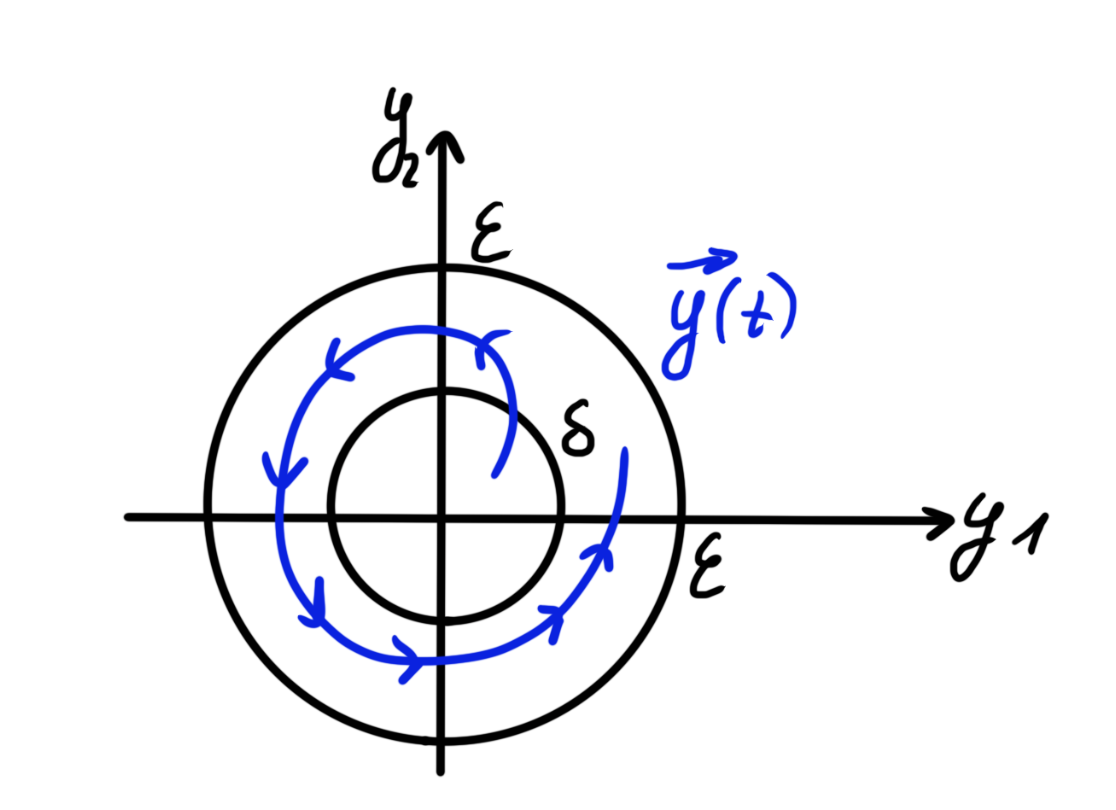
\includegraphics[width=0.3\textwidth]{/Users/vladbelousov/Desktop/Semestr_4-FP-NSU/ЭиО/Лекции_по_дням/image/48.png}
\end{center}

Пример: \( \displaystyle A_1 =1 , \text{ }  B_1= 0 , \text{ }  D_1 = -\frac{k_x}{k_z}  \) 

\[ (\overrightarrow{A_2,B_2, D_2}  ) = \left[ (\overrightarrow{A_1,B_1, D_1}  ) \times \frac{\vec{k} }{|k|} \right]\] 

\( \Rightarrow  \)  для \( \forall  \)  вектора \( \vec{k } (|\vec{k} \neq 0 |)  \exists \) плоскость \( \perp \vec{k}  \), в которой можно выбрать два линейно независимых (ортогональных) вектора \( \overrightarrow{A_1, B_1, D_1}   \)  и \( \overrightarrow{A_2, B_2, D_2} \), которые являются амплитудами собственных колебаний и имеют одну и ту же частоту:

\[ \displaystyle \underbrace{\frac{\omega ^2 \varepsilon \mu }{c ^2 }}_{k ^2} = k_x ^2 + k_y ^2 + k_z ^2 \quad \text{(т.е. двухкратное вырождение).}  \] 

Пример: если a= b, тогда решение с \( n_x, n_y ,n_z \)  имеет ту же частоту, что и решение \( n_y, n_x, n_z \to  \)  четырех кратное вырождение.

Магнитное поле моды \( n_x, n_y, n_z \):

\[ \omega_{ n_x, n_y ,n_z}  = \frac{c}{\sqrt{\varepsilon \mu}} \sqrt{\left( \frac{\pi n_x}{a}  \right) ^2+ \left( \frac{\pi n_y}{b}  \right) ^2+ \left( \frac{\pi n_z}{d}  \right) ^2} , \quad  (\varepsilon = \mathrm{cosnt} , \text{ } \mu = \mathrm{cosnt}  ) \] 

\[ \vec{B } (\vec{r } , t ) = \frac{c}{i \omega_{ n_x, n_y ,n_z}}  \mathrm{rot } \vec{E} (\vec{r}  ,t )  \] 

\section{Связь мод резонатора с плоскими волнами}

\[ E_x(\vec{r } , t ) = -\frac{A}{8}  (e^{i k_x x} +e^{-i k_x x} )(e^{i k_y y} -e^{-i k_y y} )(e^{i k_z z} -e^{-i k_z z} )e^{- i \omega t} =   \] 

\[ = c_1 e^{i k_x x + i k_y y + i k_z z - i \omega t} +c_2 e^{-i k_x x + i k_y y + i k_z z - i \omega t} +... c_8 e^{...}   \] 

- восемь плоских волн.

\begin{center}
    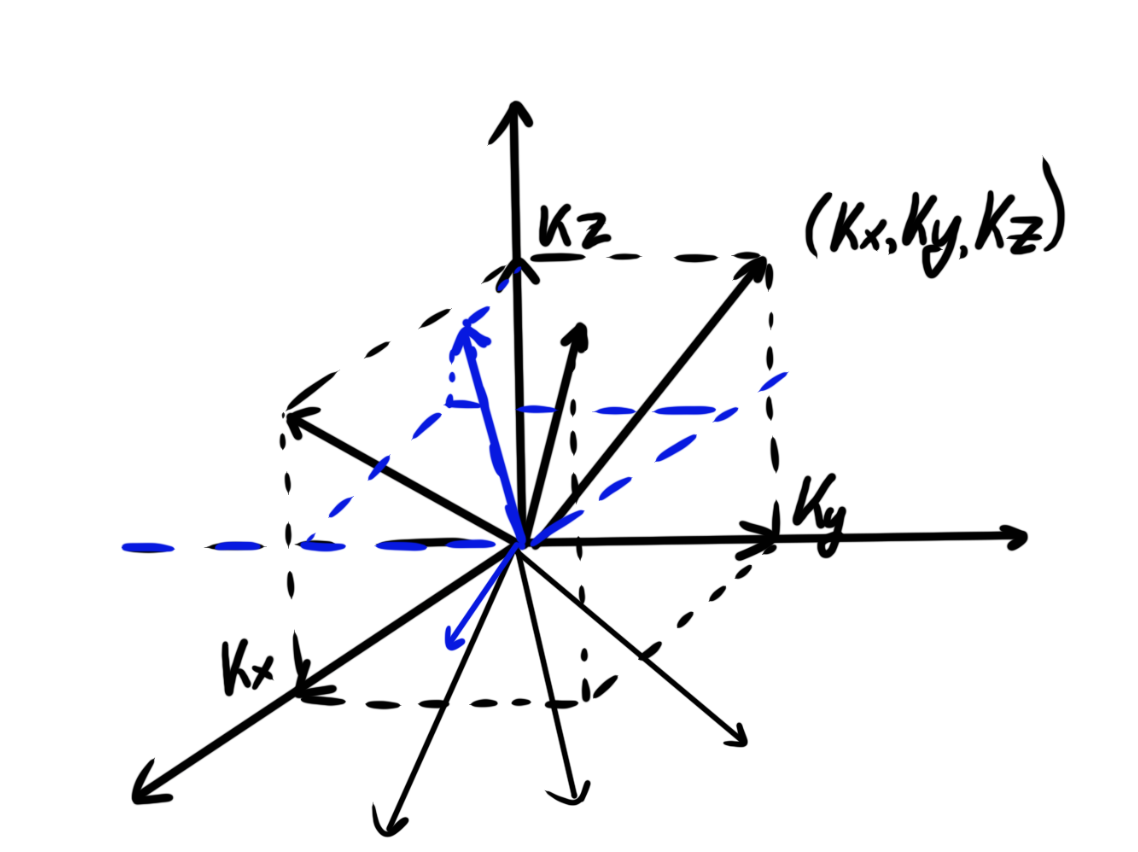
\includegraphics[width=0.5\textwidth]{/Users/vladbelousov/Desktop/Semestr_4-FP-NSU/ЭиО/Лекции_по_дням/image/49.png}
\end{center}

\section{Минимальная частота мод}

\[ \omega_{0,0,0} - \text{ не бывает} ,\quad \omega_{0,0,n_z} - \text{ не бывает } (\text{если два индекса равны 0, то решений нет} )   \] 

\[ \omega_{1,1,0} =\frac{c}{\sqrt{\varepsilon \mu } } \sqrt{\left( \frac{\pi}{a}  \right) ^2 + \left( \frac{\pi}{b}  \right) ^2}  , \quad \omega_{1,0,1} = \frac{c}{\sqrt{\varepsilon \mu } } \sqrt{\left( \frac{\pi}{a}  \right) ^2 + \left( \frac{\pi}{d}  \right) ^2} , \quad \omega_{0,1,1} = \frac{c}{\sqrt{\varepsilon \mu } } \sqrt{\left( \frac{\pi}{b}  \right) ^2 + \left( \frac{\pi}{d}  \right) ^2}  \] 


Если \( a>b>d ,  \) то \( \omega_{1,1,0}  \) - минимальная частота \( \Rightarrow  \) основная мода резонатора\dots

Поле основной моды: 

\[ E_x = E_y = 0  , \quad  \mathrm{Re}  (E_z (\vec{r } , t )) = E_0 \sin (k_x x)\sin  (k_y y)\cos (\omega_{1,1,0} t) \]

\begin{center}
    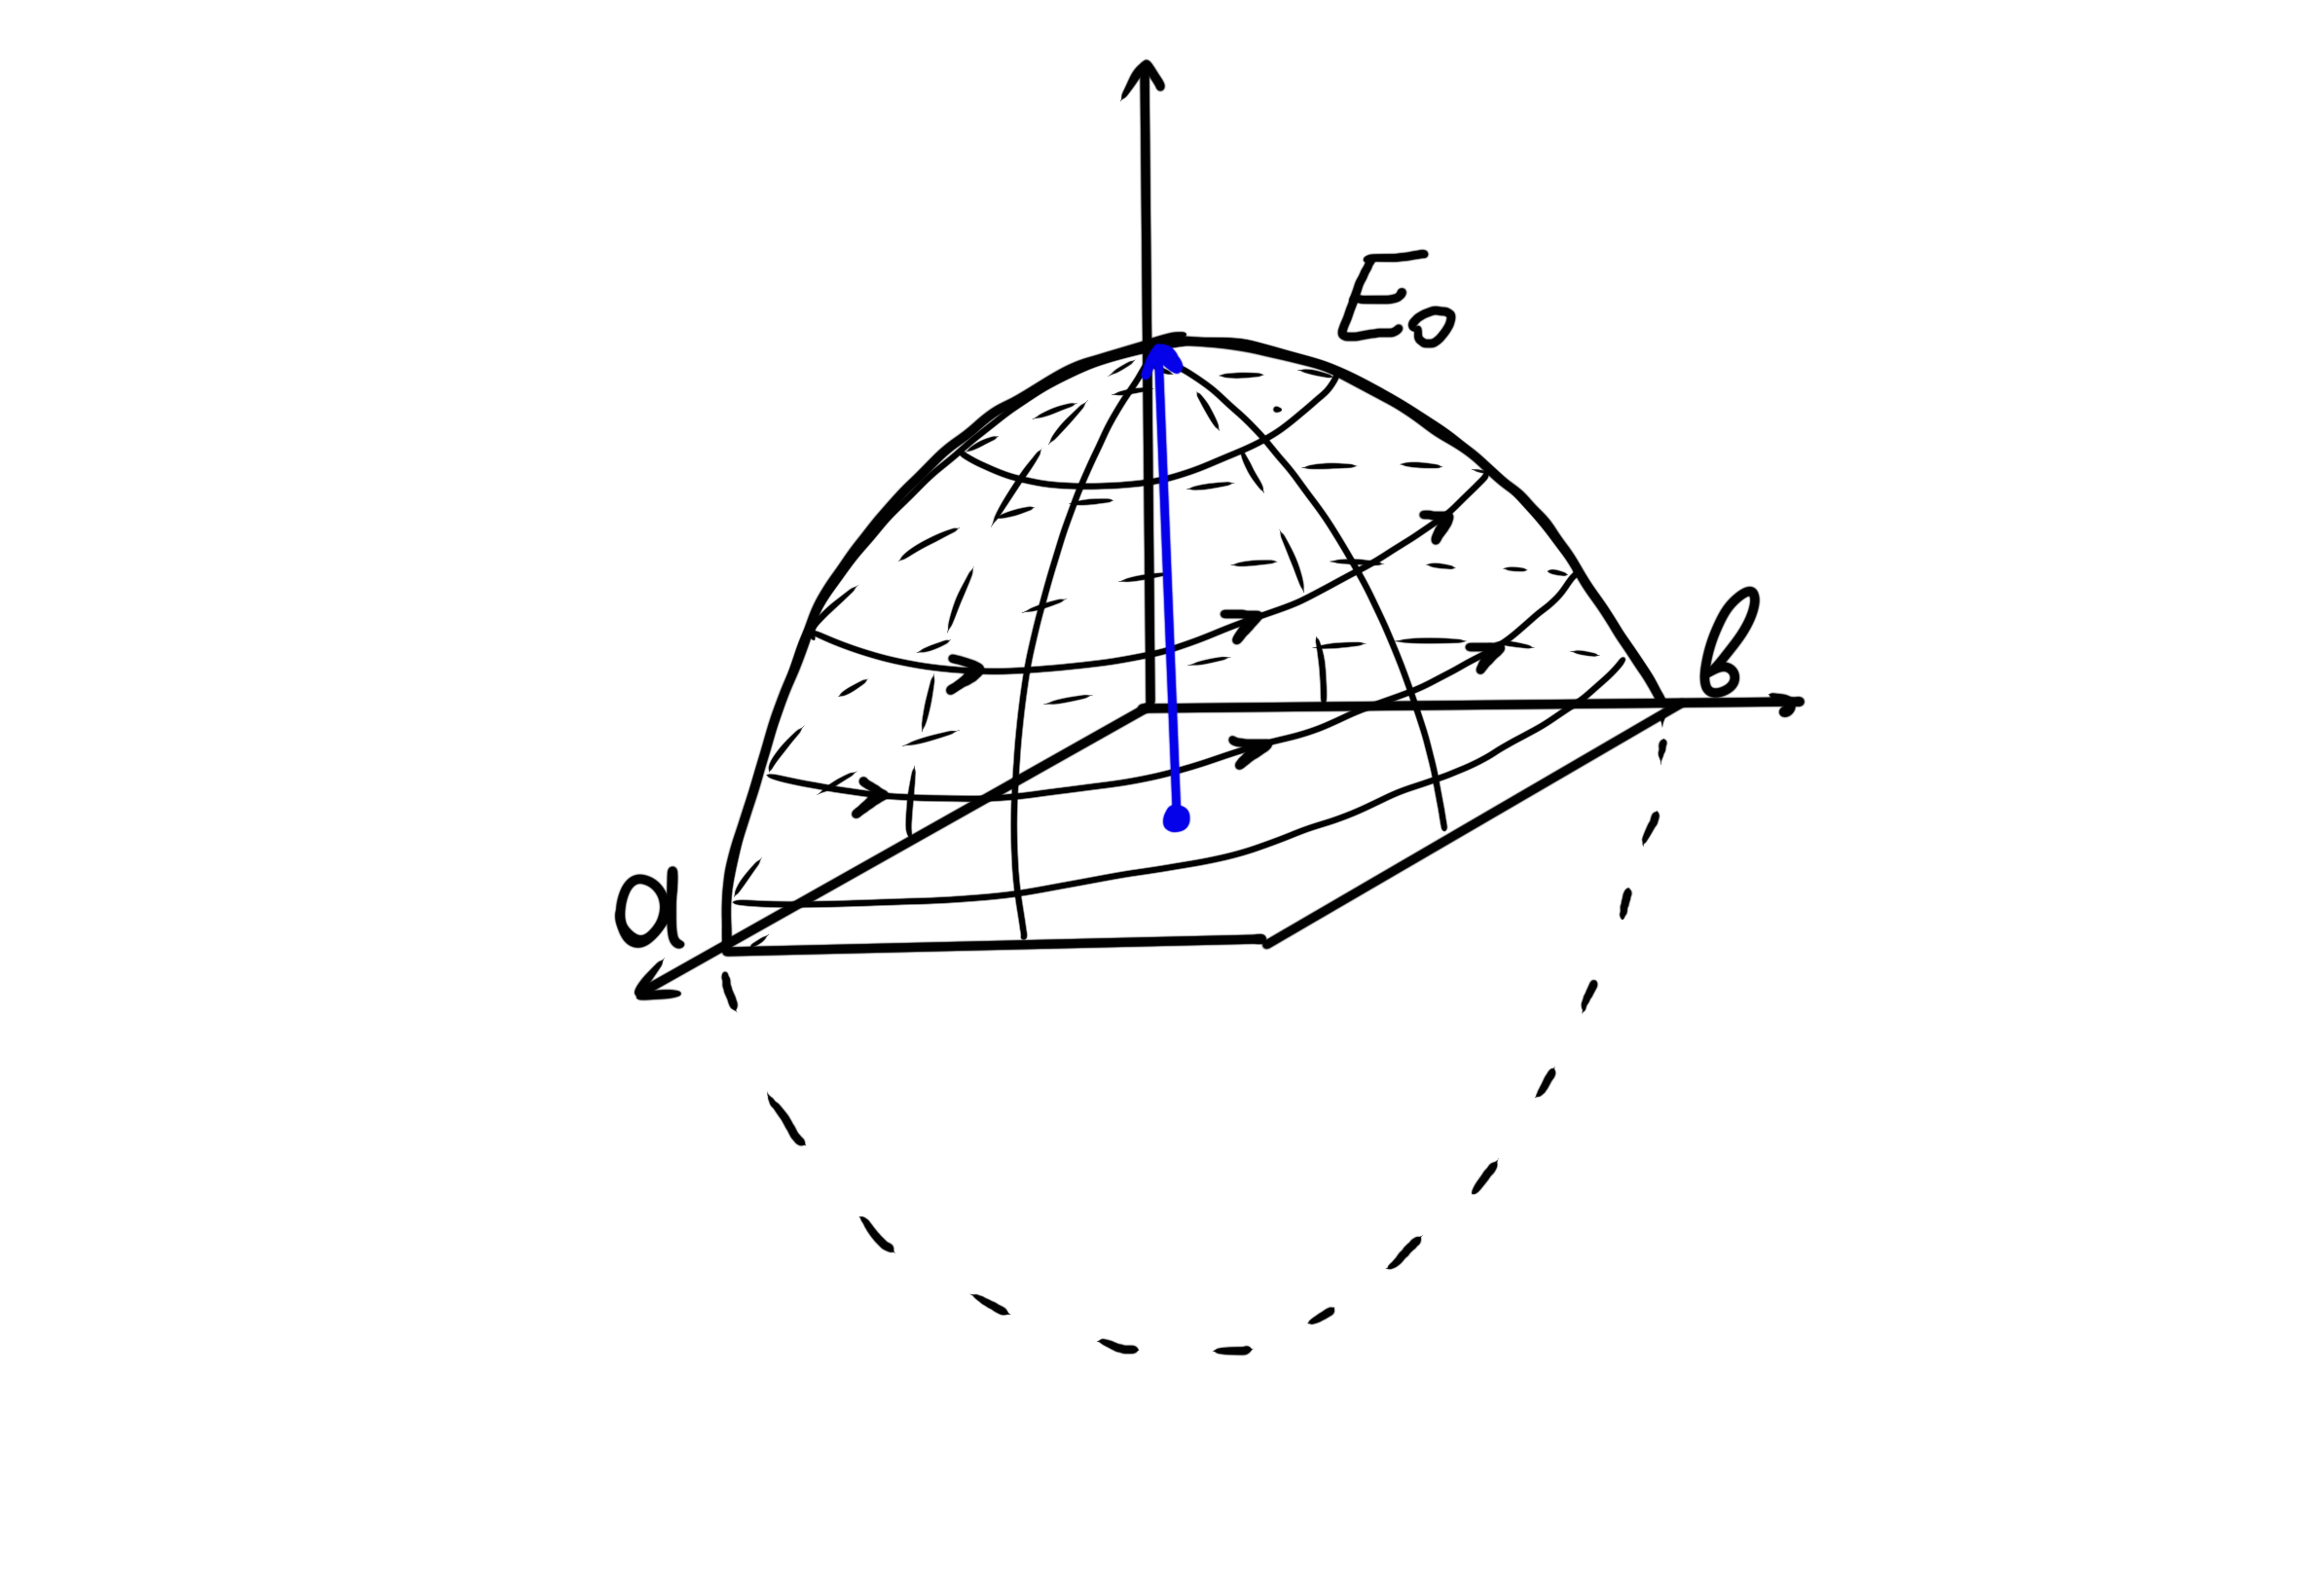
\includegraphics[width=0.5\textwidth]{/Users/vladbelousov/Desktop/Semestr_4-FP-NSU/ЭиО/Лекции_по_дням/image/50.png}
\end{center}

\[ \vec{B }  = - \frac{c}{\omega_{1,1,0} }  \left[ \vec{e_x} k_y \sin (k_x x ) \cos (k_y y ) - \vec{e_y } k_x \cos (k_x x ) \sin (k_y y )   \right]  \sin (\omega_{1,1,0} t)\] 

\section{Влияние конечной проводимости стенок на частоты мода резонатора}

Рассматриваем случай, когда электромагнитные поля мод проникают в стенки резонатора на глубину \(\displaystyle  \delta \sim \frac{c }{\sqrt{2 \pi \mu \sigma \omega}} \ll a, b,d  \). Найдем время затухания моды в резонаторе. 

\[ E,B \sim e ^{-i \omega t } = e^{ - i (\omega ' - i\omega '')t} , \text{ где } \omega' = \mathrm{Re} (\omega) , \text{ } \omega'' =-\mathrm{Im} (\omega)  \quad (\omega =\omega ' - i \omega'')   \] 

Пусть \( \varepsilon = \mathrm{cosnt}, \text{ }  \mu = \mathrm{cosnt}.   \) 

\[ \overline{W}_E - \text{(полная энергия поля в резонаторе, усредненная по t)} = \int dV \frac{\varepsilon (\overline{\mathrm{Re}\vec{E} (\vec{r } ,t ) }  ) ^2 }{8 \pi}  \boxed{=}  \] 

\[(\overline{\mathrm{Re}\vec{E} (\vec{r } ,t ) }  ) ^2 = \left( \overline{\frac{\vec{E }  (\vec{r } ) e^{- i (\omega ' - \omega '')t} + \vec{E } ^{* }  (\vec{r } ) e ^{ i \omega ' t - \omega ' t} }{2} }   \right)  \] 

\[ \boxed{= } \int  \frac{dV \varepsilon}{8 \pi}  \left\{\overline{ \frac{(\vec{E } (\vec{r }) \vec{E } (\vec{r } ) ) e^{- 2 i \omega 't } + (\vec{E } ^{* } (\vec{r } ), \vec{E } ^{* } (\vec{r } )) e ^{ 2 i \omega ' t} + 2 (\vec{E } (\vec{r } ), \vec{E} ^{* } (\vec{r } )) }{4} }   \right\} e^{- 2 \omega ''t }  \] 

\[ \overline{e ^{ -2 i \omega ' t } }  =\overline{\cos (2 \omega ' t)- i \sin (2 \omega ' t)} = 0 \quad (\text{ за период } T =\frac{ 2\pi}{\omega'} )     \] 

\[ \Rightarrow \overline{W_E} = \int dV \frac{\left\lvert \vec{E } (\vec{r } ) \right\rvert ^2 \varepsilon}{1 6\pi } e^{- 2 \omega '' t}     \] 

\[ \overline{W_B} = \int dV \frac{\left\lvert \vec{B } (\vec{r } ) \right\rvert ^2}{1 6\pi }\frac{1}{\mu}  e^{- 2 \omega '' t}    \] 


\begin{center}
    \includegraphics[width=0.4\textwidth]{/Users/vladbelousov/Desktop/Semestr_4-FP-NSU/ЭиО/Лекции_по_дням/image/52.png}
    \includegraphics[width=0.3\textwidth]{/Users/vladbelousov/Desktop/Semestr_4-FP-NSU/ЭиО/Лекции_по_дням/image/53.png}
\end{center}

\[ \overline{W }  = \overline{W_E} + \overline{W_B}  = \overline{W_0 } e^{ - 2 \omega '' t}  \quad  \frac{d \overline{ W}  }{dt } = - 2 \omega '' \overline{W }(t)  \] 

Потери энергии в стенках резонатора: \( \displaystyle \oint \left( \overline{\vec{\mathbb{S}} },ds \right)   = \frac{c}{ 16 \pi}  \sqrt{\frac{ \mu \omega '}{2 \pi \sigma} } \oint_{S} \left\lvert \vec{H } _{\tau } (\vec{r})   \right\rvert ^2 ds \,  e^{ - 2 \omega '' t} \) 

\[  \overline{\vec{\mathbb{S}}}   - \text{вектор Пойнтинга} , \quad S - \text{площадь стенок резонатора}   \] 

\[ \omega ''  = \frac{\frac{c}{ 16 \pi } \sqrt{\frac{ \mu \omega' }{2 \pi \sigma} } \displaystyle  \oint _{S} \left\lvert \vec{H } _{\tau } (\vec{r})   \right\rvert ^2 ds \, e^{- 2 \omega '' t}}{ \frac{1}{8 \pi } \displaystyle \int dV \left(  \varepsilon \left\lvert \vec{E } (\vec{r } ) \right\rvert ^2 + \frac{1}{\mu} \left\lvert \vec{B } (\vec{r } ) \right\rvert  ^2 \right)e^{- 2 \omega '' t} }   \] 

\[ Q = \frac{ \omega ' }{2  \omega '' } - \text{добротность}   \] 

Свойства резонатора с \( \omega '' = 0 (Q \to  \infty )  \)  (Ландау, Лифшиц)

\[ \int_{V} \frac{\varepsilon \left\lvert \vec{E } (\vec{r } ) \right\rvert ^2  dV}{16 \pi} = \int_{V} \frac{1}{\mu } \frac{\left\lvert \vec{B } (\vec{r } ) \right\rvert ^2  dV}{16 \pi} ,\quad   \text{ для } \varepsilon = \mathrm{cosnt}(\omega),  \text{ } \mu = \mathrm{cosnt}(\omega)    \] 

\section{Волноводы   }

- труба с идеально проводящими стенками однородная по  сечениям вдоль своей оси. Применение - транспортировка электромагнитных волн (энергии и информации) с малыми потерями на значительные расстоянияы.

\begin{center}
    \includegraphics[width=0.5\textwidth]{/Users/vladbelousov/Desktop/Semestr_4-FP-NSU/ЭиО/Лекции_по_дням/image/51.png}
\end{center}

\[ \underset{\text{поле бегущей волны} }{\vec{E } (\vec{r } , t )} \kern-20pt  = \vec{E }  ( x, y ) e^{ i k_z z  - i \omega t } , \quad  \vec{B } (\vec{r }, t          )  = \vec{B }  ( x, y ) e^{ i k_z z  - i \omega t }  \] 

\[ \mathrm{rot } (\vec{E } (x,y )e^{i k_z z}) = \frac{i \omega }{c } ( \vec{B } (x,y ) e^{ i k_z z} )     \] 

\[ \mathrm{rot } (\vec{H } (x,y )e^{i k_z z}) = -\frac{i \omega }{c } ( \vec{D} (x,y ) e^{ i k_z z} )  \] 

Выделим поперечные компоненты этих уравнений: 

\[[ \vec{e_{z} } \times [ \nabla \times  \vec{E } (x,y ) e^{i k_z z} ]] = \frac{i \omega }{c } [ \vec{e_z } \times  \vec{B } (x,y) e^{ i k_z z}  ]  , \quad  \begin{aligned}
    \vec{B } (x,y ) = \mu(\omega ) \vec{H}(x,y ) \\ 
    \vec{D} (x,y ) = \varepsilon(\omega ) \vec{E}(x,y )
\end{aligned}    \] 

\[ \nabla (E_z (x,y ) e^{ i k_z z } ) - \frac{\partial}{\partial z} (\vec{E } (x,y )e^{i k_z z} ) = \frac{i \omega }{c } [\vec{e_z} \times \vec{B } (x,y ) e^{ i k_z z} ]\text{  }  (z-\text{ая компонента уравнения } \equiv 0)  \] 

\[ (\nabla_{\perp } E_z (x,y ) ) e^{i k_z z} - i k_z \vec{E } _{ \perp } (x,y ) e^{i k_z z} =   \frac{ i \omega }{c } [ \vec{e_z} \times  \vec{B} _{ \perp } (x,y ) ]     \] 

\[ \nabla_{ \perp } H_z (x,y )- H_{ \perp } (x,y ) i k_z = - \frac{ i\omega }{c } [\vec{e_z}\times \vec{D } _{\perp  } (x,y)  ] \] 

\( \nabla_{ \perp }  \) - двумерный вектор (\( \frac{\partial}{\partial  x},\frac{\partial}{\partial y}   \)), \( \vec{E}_{ \perp } (x,y) \) - поперечная составляющая волны \( \vec{E }  \).

%%-------------------------------%%

% Закрытие документа, если файл компилируется отдельно
\ifdefined\mainfile
    % Если это основной файл, не нужно заканчивать документ
\else
    \end{document}
\fi
% Условная компиляция для самостоятельной работы
\ifdefined\mainfile
    % Если это часть основного файла, не добавляем начало и конец документа
\else
    \documentclass[12pt, a4paper]{report}
    \usepackage{/Users/vladbelousov/Desktop/Semestr_4-FP-NSU/Настройка/library}
    \usepackage[utf8]{inputenc} % Подключение поддержки UTF-8
    \begin{document}
\fi

%%-------------------------------%%

\section{Продолжение ЭМ-волн в волноводах}

\[ \vec{E } (\vec{r } ,t ) = \vec{E } (x, y ) e^{ i k_z z - i \omega y }, \text{ } \vec{B } (\vec{r } , t )= \vec{B } (x,y) e^{  i k_z z - i \omega t}    \] 

\[ \nabla_{ \perp  } (E_z (x,y ) e^{ i k_z z })   - \frac{\partial}{\partial  z } (\vec{E } _{ \perp } (x,y ) e^{ i k_z z }) =  \frac{ i \omega}{c }[ \vec{e_z} \times  \vec{B} _{ \perp } (x,y ) e^{ i k_z z}  ]   \] 

\[ 1)\quad  \nabla_{ \perp } E_z (x, y ) - i k_z \vec{E } _{\perp  } (x,y   ) = \frac{ i \omega }{c } [ \vec{e_z} \times  \vec{B} _{ \perp } (x,y ) ]   \] 

\( \displaystyle \mathrm{rot } \vec{H } = \frac{i \omega \varepsilon (\omega)}{c } \vec{E}  \to  \)  домножим на \( \displaystyle \mu (\omega)  \Rightarrow \mathrm{rot } \vec{B } = - \frac{i \omega }{c } \varepsilon (\omega ) \mu (\omega) \vec{E }   \), далее аналогично домножаем векторно на \( \vec{e_z}  \)  и выделяем \( \perp  \) составляющую: 

\[ 2) \quad \nabla_{ \perp } B_z (x,y ) - i k_z \vec{B } _{\perp } (x,y ) = - \frac{i \omega }{c } \varepsilon \mu [\vec{e_z} \times  \vec{E} _{ \perp } (x,y ) ]   \] 

Из 1) выражаем \( \vec{E_{\perp }}   \) и подставляем в 2):

\[ \nabla_{ \perp } E_z (x,y ) - i k_z \vec{E }_{\perp  }(x,y ) = \frac{i \omega }{c } \left[ \vec{e_z} \times \left( \frac{\nabla_{ \perp } B_z (x,y )  + \frac{i \omega \varepsilon \mu}{c } [\vec{e_z} \times  \vec{E} _{ \perp }]  }  {i k_z}  \right) \right] ;     \] 

\[ [\vec{e_z }\times [\vec{e_z }\times  \vec{E } _{\perp  }  ]  ] = \vec{e_z } \cancelto{0}{(\vec{e_z }, \vec{E }_{\perp  }   )} - \vec{E } _{ \perp }  \] 

\[ i k_z \nabla_{ \perp  } E_z (x,y ) + k_z ^2 \vec{E } _{\perp  } (x,y ) = \frac{ i \omega }{c } [ \vec{e_z } \times \nabla_{ \perp  } B_z (x,y )  ] + \frac{ \omega ^2 \varepsilon \mu }{c ^2 }  \vec{E }_{ \perp }     ( x,y ) ; \quad \ae ^2 = \frac{ \varepsilon (\omega )\mu (\omega ) \omega ^2 }{c ^2 }   - k_z ^2   \] 

\[ \vec{E } _{\perp  } (x,y) = \frac{i k_z }{ \ae ^2 } \nabla_{ \perp } E_z (x,y ) - \frac{ i \omega }{c \ae ^2  } [ \vec{e_z  } \times  \nabla_{ \perp } B_z (x,y ) ]     \] 

Аналогично:

\[ \vec{B } _{\perp } (x,y )= \frac{i k_z }{ \ae ^2 } \nabla_{ \perp } B_z (x,y ) + \frac{ i \omega \varepsilon \mu }{c \ae ^2  } [ \vec{e_z  } \times  \nabla_{ \perp } E_z (x,y ) ]     \] 

Уравнения на \( E_z (x,y ) \) и \( B_z (x,y ) \):

\[ \begin{aligned}
\begin{cases}
    \displaystyle \mathrm{rot }(\mathrm{rot }\vec{E } ) = \frac{ i \omega }{c } \mathrm{rot } (\mu \vec{H } ) = \frac{ i \omega }{c }\mu \left( - \frac{ i \omega \varepsilon }{c}  \right) \vec{E}  \\
    \displaystyle \mathrm{rot }(\mathrm{rot }\vec{E } ) = \cancelto{0}{\nabla \mathrm{div } \vec{E }} - \Delta \vec{E }  , \quad  \mathrm{div } \vec{D } = 0 = \mathrm{div } (\varepsilon \vec{E }) = \varepsilon \mathrm{div } \vec{E }  =0  
\end{cases}
\quad   \Rightarrow
\end{aligned} \] 

\[ \Rightarrow  \Delta \vec{E } (x,y,z ) + \frac{ \omega ^2 \varepsilon \mu }{c  ^2 } \vec{E } (x,y,z ) = 0  \] 

\[ \left( \frac{\partial ^2}{\partial  x ^2 }+ \frac{\partial ^2}{\partial  y ^2 } +\frac{\partial ^2}{\partial  z ^2 }   \right) E_z (x,y ) e^{ i k_z z } + \frac{ \omega ^2 }{ c ^2 } \varepsilon \mu E_z (x,y ) e^{ i k_z z } = 0  \] 

\[ \Delta_{\perp  } E_z (x,y ) e^{ i k_z z } - k_z ^2 E_z (x,y  ) e^{ i k_z z }  + \frac{\omega ^2 \varepsilon \mu }{c ^2 } E_z (x,y ) e^{ i k_z z } = 0     \] 

\[ \Delta_{\perp  } E_z (x,y )  + \ae ^2 E_z (x,y  )  = 0    - \text{ двумерное волновое уравнение}  \] 

\[ \text{Аналогично: } \Delta_{ \perp  } B_z (x,y ) + \ae ^2 B_z (x,y ) = 0 \] 

Граничные условия: 
\begin{center}
    \includegraphics[width=0.3\textwidth]{/Users/vladbelousov/Desktop/Semestr_4-FP-NSU/ЭиО/Лекции_по_дням/image/54.png}
\end{center}
\[ 1) E_{\tau }|_{\text{Г} }  = 0 \Rightarrow (\vec{E } , \vec{r } ) = 0  ,\quad  (\tau -\text{ вдоль поверхности}) , \quad 2) B_{n } |_{\text{Г} } = 0  \Rightarrow (\vec{n } , \vec{B } )|_{\text{Г} } = 0  \] 

\[1) \text{Пусть } \vec{\tau } \parallel \vec{e_z } \Rightarrow E_z (x,y ) e^{i k_z z - i \omega t} |_{\text{Г} } = 0 \Rightarrow E_z (x,y ) |_{\text{Г} } = 0    \] 

\[ \text{Пусть }\vec{\tau} \cancel{\parallel} \vec{e_z } \Rightarrow E_{\tau }  = ( \vec{\tau }, (\vec{e_z }E_z + \vec{E } _{\perp }  ) ) |_{\text{Г} } = \underbrace{(\vec{\tau }, \vec{e_z}  ) \cancelto{0}{E_z}|_{\text{Г} }}_{0}  +(\vec{\tau }, \vec{ E } _{\perp }  )=   \] 

\[ = \left( \vec{\tau} , \left\{ \frac{i k_z }{\ae ^2 } \nabla_{ \perp } E_z(x,y ) - \frac{ i \omega }{c \ae ^2 } [ \vec{e_z } \times  \nabla_{ \perp } B_z (x,y )  ]   \right\} \right)  \bigg | _{\text{Г} }  = \frac{ i k_z }{\ae ^2 } \frac{\partial  E_z}{\partial \tau }\bigg | _{\text{Г} } - \frac{ i \omega  }{c \ae ^2 } ( \vec{\tau }, [ \vec{e_z } \times  \nabla_{ \perp } B_z (x,y )] ) \bigg | _{\text{Г} } =\] 

\[ \pm  \frac{ i \omega }{c \ae ^2 }( \nabla B_z , \vec{n } ) \bigg | _{\text{Г} }  = \pm  \frac{ i \omega  }{c \ae ^2 } \frac{\partial  B_z(x,y )}{\partial  \vec{n}  } \bigg | _{\text{Г} } = 0 \Rightarrow E_z (x,y )\bigg | _{\text{Г} } = 0, \frac{\partial  B_z}{\partial  \vec{n}  }  \bigg | _{\text{Г} } = 0   \] 



\[2) \text{ }  (\vec{n } , \vec{B } ) \bigg | _{\text{Г} } = 0 \Rightarrow \left( \vec{n } , \left\{ \vec{e_z }B_z (x,y ) + \frac{ i k_z }{\ae ^2 } \nabla_{ \perp } B_z (x,y ) + \frac{ i \omega \varepsilon \mu }{c  \ae ^2 } [ \vec{e_z }\times  \nabla_{ \perp } E_z (x,y ) ]    \right\} \right) \bigg | _{\text{Г} } =\] 

\[= \frac{i k_z }{\ae ^2 } \frac{\partial  B_z (x,y )}{\partial \vec{n} } \bigg | _{\text{Г} } + \frac{ i \omega \varepsilon \mu}{ c \ae ^2 } ( \vec{n }, [ \vec{e_z } \times  \nabla_{ \perp } E_z (x,y )] ) \bigg | _{\text{Г} }   =\frac{ i \omega \varepsilon \mu  }{c \ae ^2 } (\nabla_{ \perp } E_z (x,y), [\vec{n} \times  \vec{e_z}  ]  )= \frac{ i \omega \varepsilon \mu  }{c \ae ^2 } \frac{\partial  E_z (x,y )}{\partial  \vec{\tau}  } \bigg | _{\text{Г} } = 0  \] 

Итог: первое и второе граничные условия выполняются при одинаковых условиях.

Для упрощения анализа разделим общее решение на два: 

1-ый тип: \( E  \) - волна (ТМ - волна) \( E_z (x,y  ) \neq 0 , B_z (x,y  ) = 0  \)  внутри волновода;

2-ой тип: \( H  \) - волна (ТЕ - волна) \( E_z (x,y  ) = 0 , B_z (x,y  ) \neq 0  \). 

Для \( E  \) - волны: \(\Delta_{ \perp  } E_z (x,y  ) + \ae ^2 E_z (x,y ) = 0 + \text{ Г.У } E_z |_{\text{Г} }   = 0 \) 

- задача Штурмана-Лиувилля, из решения которой находятся собственные значения \( \ae_{n } , n= ...;\) и собственные функции \( E_{z } ^{(n )}  (x,y) = ...; \) 

Для \( H  \) - волны: \(\displaystyle  \Delta _{\perp } B_z (x,y) + \ae ^2 B_z (x,y ) = 0 + \text{ Г.У. } \frac{\partial  B_{z } }{\partial  n } \bigg|_{\text{Г} } =0   \) 

Пример 1: \( H  \) - волна в прямоугольном волноводе

\begin{center}
    \includegraphics[width=0.4\textwidth]{/Users/vladbelousov/Desktop/Semestr_4-FP-NSU/ЭиО/Лекции_по_дням/image/55.png}
\end{center}
\[ \left(  \frac{\partial  ^2 }{\partial  x ^2 } + \frac{\partial  ^2 }{\partial  y  ^2 }   \right) B_z (x,y ) + \ae ^2 B_z (x,y) = 0 , \text{  } + \text{ Г.У. } \frac{\partial  B_{z } }{\partial  n } \bigg|_{\text{Г} } =0  \Rightarrow \frac{\partial  B_z }{\partial  x }\bigg|_{x=0,a} = 0, \text{ } \frac{\partial  B_z }{\partial  y }\bigg|_{y=0,b} = 0     \] 

Пусть \( B_z (x,y  )= B_1(x)B_2(y) \) 

\[ B_2(y )B_1 '' (x) + B_1( x) B_2 '' (y )+ \ae ^2 B_1(x) B_2(y ) = 0 \] 

\[ \Rightarrow \underbrace{\frac{ B_1 '' (x )}{B_1 (x)} }_{=\mathrm{const} = -k_x ^2   }+\underbrace{\frac{ B_2 '' (y )}{B(y )}}_{=\mathrm{const}= - k_y ^2  } + \ae ^2 = 0   \Rightarrow \begin{cases}
    B_z (x,y ) = B_0 \sin (k_xx \alpha_x  ) \sin ( k_y y \alpha_y ) \\ 
    \ae ^2 = k_x ^2 + k_y ^2 
\end{cases} \] 

Граничные условия: 

\[ \frac{\partial  B_z }{ \partial  x } \bigg | _{x = 0  } = k_x B_0 \cos \alpha_x \sin  (k_y y + \alpha_y ) = 0 \text{ при } \forall  y \Rightarrow \alpha_x = \frac{\pi}{2}     \] 

\[ \frac{\partial  B_z }{\partial  x } \bigg | _{x = a  } = k_x B_0 \cos (k_x a + \frac{\pi}{2 } )\sin( k_y y + \alpha_y ) = 0 \Rightarrow k_x a = n_x \pi, \text{ }  k_x =  \frac{ n_x \pi } {a } , \text{ }  n_x \in  \mathbb{Z} \] 

\[ \text{Аналогично: }  \alpha_y = \frac{\pi}{2 } , \text{ } k_y = \frac{ n_y \pi } {b } , \text{ }  n_y \in  \mathbb{Z} \Rightarrow \ae_{n_x, n_y } = \sqrt{\left( \frac{n_x \pi }{a }  \right) ^2 + \left( \frac{n_y \pi }{b } \right) ^2} - \text{собственные числа} \] 

\[ B_z (x,y  ) = B_0 \cos (k_x x ) \cos (k_y y ) , \text{ }  B_z(\vec{r }  ,t )= B_0 \cos (k_x x ) \cos (k_y y) e^{i k_z z - i \omega t} \] 

\[ E_{\perp } (x,y  ) = - \frac{i \omega  }{c \ae _{n_x, n_y } ^2 }[\vec{e_z  }  \times  \nabla_{ \perp } B_z (x,y ) ] , \text{ } B_{ \perp  } (x,y )= \frac{ i k_z }{\ae_{n_x, n_y } ^2 } \nabla_{ \perp } B_z(x,y)    \] 

\[ \nabla_{ \perp } B_z(x,y) = \left( \vec{e_x } \frac{\partial  }{\partial  x } + \vec{e_y } \frac{\partial  }{\partial  y }   \right) B_z(x,y )=- B_0 \left\{ \vec{e_x }k_x \sin (k_x x ) \cos (k_y y ) + \vec{e_y }k_y \cos (k_x x ) \sin (k_y y )  \right\} \] 

Какие \( n_x, n_y  \) допустимы?  Пусть \( n_x = 0 , n_y = 0 \) 

\[\textcolor{red}{B_z(\vec{r },t ) = B_0 e^{i k_z z - i \omega t }, \text{ } \vec{B } _{\perp  }(\vec{r } ,t ) = \frac{ i k_z }{0 ^2 } 0 - \text{ проверить из уравнений Максвелла, что  } B_{\perp  } = 0    }   \] 

\[ \mathrm{div} \vec{B } = 0 = \frac{\partial  B_z }{\partial  z } = i k_z B_0 e^{i k_z z - i \omega t } (k_z \neq 0 ) \Rightarrow B_0 \text{ } (\text{такой моды нет} )   \] 

Пусть: \( \displaystyle  n_x = 1 , n_y = 0  \Rightarrow \ae _{1,0 } = \frac{\pi}{a}, \text{   }  \frac{ \omega_{1,0 } ^2 \varepsilon \mu }{c ^2 } = \left(  \frac{\pi }{a }  \right) ^2 + k_z ^2  \) 

\[ B_z ( x,y ) = B_0 \cos (k_x x ) ,\text{ } B_{\perp  } (x,y) = \frac{i k_z }{\ae_{1,0} ^2 } B_0 (- k_x  )\sin (k_x x )\vec{e_x} , \text{  далее } \to  \begin{cases}
\varepsilon(\omega ) = \mathrm{const }  \\
\mu (\omega ) = \mathrm{const } 
\end{cases}    \] 

\[ \vec{E } _{ \perp  }(x,y ) = - \frac{ i\omega }{c \ae ^2 } \vec{e_y }B_0 (-k_x )\sin (k_xx)    \] 

\begin{center}
    \includegraphics[width=0.5\textwidth]{/Users/vladbelousov/Desktop/Semestr_4-FP-NSU/ЭиО/Лекции_по_дням/image/56.png}
\end{center}

- мода\( _{1,0}  \) - основная мода волновода.

\[ v_{\Phi } = \frac{ \omega } {k_z }, \text{  } v_{g } = \frac{ d \omega }{d k_z}   \]

\[ v_{\Phi } v_g = \frac{ c ^2 }{\varepsilon \mu}   \] 

\[ v_{\Phi } = tg \alpha , \text{ }  v_g =  tg \beta \] 

Представление в виде плоских волн: 

\[ B_z (\vec{r }, t ) = B_0 \left( \frac{ e^{i k_x x } + e^{-i k_x x } }{2} \right) e^{i k_z z - i \omega t}  = \frac{B_0 }{2 } e^{ i k_xx + i k_z z - i \omega t} +  \frac{B_0 }{2 } e^{-i k_xx - i k_z z - i \omega t}\]

\begin{center}
    \includegraphics[width=0.5\textwidth]{/Users/vladbelousov/Desktop/Semestr_4-FP-NSU/ЭиО/Лекции_по_дням/image/57.png}
\end{center}

\[ v_{\Phi } = \frac{c }{ \sqrt{\varepsilon \mu   }\cos \gamma}  , \quad  v_g = \frac{c }{ \sqrt{\varepsilon \mu  }}\cos \gamma , \cos \gamma = \frac{ k_x }{\sqrt{k_x ^2 + k_z ^2 }}   \] 



%%-------------------------------%%

% Закрытие документа, если файл компилируется отдельно
\ifdefined\mainfile
    % Если это основной файл, не нужно заканчивать документ
\else
    \end{document}
\fi
%Март
% Условная компиляция для самостоятельной работы
\ifdefined\mainfile
    % Если это часть основного файла, не добавляем начало и конец документа
\else
    \documentclass[12pt, a4paper]{report}
    \usepackage{/Users/vladbelousov/Desktop/Semestr_4-FP-NSU/Настройка/library}
    \usepackage[utf8]{inputenc} % Подключение поддержки UTF-8
    \begin{document}
\fi

%%-------------------------------%%


\section{Продолжение: \( E \) волна в прямоугольном волноводе }

\[ E_z \neq 0 , \text{ } B_z = 0 \] 

\[ \Delta_{ \perp  } E_z ( x,y ) + \ae ^2 E_z (x,y )= 0  \] 

\[ \text{Г.У } E_z|_{\text{Г} } = 0 \Rightarrow E_z (x,y ) = E_1 (x) E_2 (y )  \] 

\[ \underbrace{\frac{E_1 '' (x )}{E_1 (x ) }}_{-k_x ^2 } + \underbrace{\frac{ E_2 ''(y )}{E_2 (y )}}_{- k_y ^2 } + \ae ^2 = 0 \Rightarrow E_z (x,y) = E_0 \sin (k_x x + \alpha_x ) \sin (k_y y + \alpha_y)   \] 

\[ \text{Г.У } E_z |_{y= 0 , \text{ }  y = b } = 0 \Rightarrow \alpha_y = 0 , \text{ } k_y b = n_y \pi , \text{ }  E_z |_{x= 0 , \text{ } x =a  }  \Rightarrow \alpha_x = 0 , \text{ } k_x a = n_x \pi ,  \text{ } n_x ,n_y \in \mathbb{Z}  \] 

\[ E_z (\vec{r } ,  t ) = E_0 \sin (k_x x) \sin (k_y y )e^{ i k_z z - i \omega_{n_x, n_y } t } , \quad  \frac{\omega_{n_x, n_y } ^2  \varepsilon \mu}{c ^2} = k_x ^2 + k_y ^2 + k_z ^2    \] 

Мода минимальной частоты: \( E_{11}     \text{ } (n_x = 1, \text{  } n_y= 1 ) \) 

\section{ТЕМ-волны в неодносвязных волноводах }

\begin{center}
    \includegraphics[width=0.3\textwidth]{/Users/vladbelousov/Desktop/Semestr_4-FP-NSU/ЭиО/Лекции_по_дням/image/59.png}
\end{center}

\begin{center}
    (1) - односвязный волновод, (2) - двухсвязный волновод;
\end{center}

В (2) помимо \( E \) и \( H  \) - волн существует ТЕМ-волна, с \( E_z = 0, \text{ } B_z = 0 \). Дисперсионное соотношение так же как для плоских монохроматических волн в свободном растворе: 

\begin{center}
    \includegraphics[width=0.3\textwidth]{/Users/vladbelousov/Desktop/Semestr_4-FP-NSU/ЭиО/Лекции_по_дням/image/58.png}
\end{center}

\begin{center}
    для случая \( \varepsilon (\omega )= \mathrm{const}, \text{ } \mu( \omega ) = \mathrm{const}     \) 
\end{center}

\[ \frac{ \omega ^2 }{c ^2 } \varepsilon \mu = k_z ^2   \]

\[ \vec{E } _{\perp  }( \vec{r }, t      ) = \vec{E } (x,y )e^{ i k_z z - i \omega t }   \] 

\[ \vec{B } _{\perp  }(\vec{r } ,t ) = \vec{B } (x,y )e^{ i k_z z - \omega t}   \] 

\[ \left( \mathrm{rot }   \vec{E }  \right)_{z }  = \frac{ i \omega }{c } (\vec{B } )_z = 0 \Rightarrow \frac{\partial  E_y } {\partial  x } - \frac{ \partial  E_x }{\partial  y} = 0 , \text{  ищем решение в таком виде:  } \vec{E} = - \nabla_{ \perp }  \varphi     \] 

\[ E_x = - \frac{\partial  \varphi }{\partial x }, \text{  } E_y = - \frac{\partial  \varphi}{\partial  y } \Rightarrow \frac{ \partial  }{\partial  x }\left( - \frac{\partial  \varphi }{\partial  y }  \right)    - \frac{ \partial  }{\partial y  }\left( - \frac{\partial  \varphi }{\partial  x }  \right) = 0 \] 

\[ \mathrm{div } \vec{E } = 0 = \frac{\partial  E_x }{\partial  x } + \frac{\partial  E_y }{\partial  y }  = \left[ \frac{\partial  ^2 \varphi }{\partial  x ^2 }+ \frac{\partial  ^2 \varphi }{\partial  y ^2 }   \right] = 0 \Rightarrow \Delta_{\perp  }  \varphi =0   \] 

Из \( E_{\tau } | _{\text{Г} }  \Rightarrow \varphi|_{\text{Г} } = \mathrm{const}     \) 

Почему в односвязном волноводе нет таких волн: 

\begin{center}
    \includegraphics[width=0.2\textwidth]{/Users/vladbelousov/Desktop/Semestr_4-FP-NSU/ЭиО/Лекции_по_дням/image/60.pdf}
\end{center}

Из теоремы единственности \( \varphi     = \mathrm{const}   \) в \( \Omega  \Rightarrow - \nabla _{ \perp } \varphi = 0\) 

Для многосвязных волноводов

\begin{center}
    \includegraphics[width=0.3\textwidth]{/Users/vladbelousov/Desktop/Semestr_4-FP-NSU/ЭиО/Лекции_по_дням/image/61.pdf}
\end{center}

\textbf{Коаксиальный волновод (кабель):} 

\begin{center}
    \includegraphics[width=0.3\textwidth]{/Users/vladbelousov/Desktop/Semestr_4-FP-NSU/ЭиО/Лекции_по_дням/image/61.png}
\end{center}

\[ \Delta _{ \perp  }\varphi = 0 \Rightarrow \frac{1}{r } \frac{\partial  }{\partial  r }\left(  r \frac{ \partial  \varphi }{\partial  r }  \right) + \frac{1}{r ^2 } \frac{\partial  ^2 \varphi }{\partial  \alpha ^2 }  =0   \] 

Зависимость от \( \alpha \) исключим \( \displaystyle \Rightarrow \frac{d \varphi }{dr  } =\frac{A }{r} , \text{ } A = \mathrm{const} \Rightarrow \varphi (r ) = A \ln r + B   \) 

\[ \varphi|_{r = b} =  0 ,\text{ } \varphi |_{r = b} =U \Rightarrow A \ln  b + B = 0 , \text{ } A \ln b = U \Rightarrow A = \frac{U }{\ln  \frac{a}{b} } , \text{ } B = -A \ln b   \] 

\[ \varphi(r ) = \frac{U }{\ln \frac{a}{b } } \ln \frac{r}{b }  = \frac{U }{\ln \frac{b}{a} } \ln \frac{b}{r}  , \text{ }  E_{r }  = - \frac{\partial  \varphi }{\partial  r } = \frac{U }{\ln \frac{b}{a} } \frac{1}{r}    \] 

\[ \vec{E } (\vec{r } ,t ) = \vec{e_r } \frac{U }{\ln \frac{b}{a} } \frac{1}{r} e^{i k_z z - i\omega t } ; \text{ } \vec{B } = \frac{c}{i \omega} \mathrm{rot } \vec{E } = \frac{c}{i \omega } i k_z  \frac{U }{\ln \frac{b}{a} } \frac{1}{r} e^{i k_z z - i \omega t }\vec{e } _{\alpha}   , \text{ } \frac{ \omega \sqrt{\varepsilon \mu } }{c } = k_z         \] 

\[ \vec{E } (\vec{r } ,t ) = \vec{e } _{\alpha } \sqrt{ \varepsilon \mu }  \frac{U }{\ln \frac{b}{a} } \frac{1}{r} e^{i k_z z - i \omega t }   \] 

\begin{center}
    \includegraphics[width=0.3\textwidth]{/Users/vladbelousov/Desktop/Semestr_4-FP-NSU/ЭиО/Лекции_по_дням/image/62.png}
\end{center}

\chapter{Геометрическая оптика}

\section{Распространение волн в неоднородных средах}

Рассмотрим только монохроматические электромагнитные волны \( \varepsilon ( \omega , \vec{r } ) , \text{ }  \mu (\omega ,\vec{r} ) \), будем рассматривать частный случай при заданной \( \omega \Rightarrow \varepsilon (\vec{r } ), \mu ( \vec{r } ) \). 

Малый параметр \(\displaystyle  \varepsilon \sim  \frac{ \lambda\text{ - характерная длина волны} }{L \text{  - масштаб неоднородности среды}}  \ll 1   \).

Решение уравнений Максвелла для однородной системы: \( \begin{aligned}
\vec{E } (\vec{r },t     ) = \vec{E }_0  e^{i (\vec{k } ,\vec{r}) - i \omega t  }  , \text{  }  \vec{E }_0 \perp \vec{k } \\
\vec{B } (\vec{r },t     ) = \vec{B }_0  e^{i (\vec{k } ,\vec{r}) - i \omega t  }  , \text{  }  \vec{B }_0 \perp \vec{k } \\
\end{aligned} \) 


Искривления изображения в нагретом воздухе \( \Rightarrow \)  отклонение волн от прямолинейного распространения.

1) Зависимости \( \vec{E } _0  \) и \( \vec{B } _0  \) от \( \vec{r } | \)  Связь \( k \) и \( \omega \): \( \displaystyle  k ^2 = \frac{ \omega ^2 } { c ^2 }\varepsilon \mu \Rightarrow k = \frac{\omega }{c } n(\omega)   \) 

\begin{center}
    \includegraphics[width=0.3\textwidth]{/Users/vladbelousov/Desktop/Semestr_4-FP-NSU/ЭиО/Лекции_по_дням/image/63.png}
\end{center}

\[ \Delta \varphi (\text{сдвиг по фазе} ) = k_1 \Delta r_1 + k_2 \Delta r_2 +... + \sum  k_i \Delta r_i = k_0 \sum n_i \Delta r_i = k_0 \underset{\text{оптический путь} }{\int_{1 }^{2 } n(\vec{r } )ds }= \psi (\vec{r} ) -\] 

- скалярная функция \( \vec{r}  \) - эйконал.

Пусть \( \vec{E } ( \vec{r } ,t ) = \vec{E } _0  \cdot e^{ i k_0 \psi (\vec{r } ) - i \omega t}  \to  \text{ в уравнение Максвелла} \), где \( \vec{E } _0\text { медленная функция от  } \vec{r }   \),  изменяется на масштабе \( L  \).

\[ \mathrm{rot } \left[ \vec{E_0 }(\vec{r } ) e^{i k_0 \psi (\vec{r } )- i \omega t }   \right] = -\frac{1}{c} \frac{\partial  }{\partial  t } \left[ \vec{B }_0 e^{i k_0 \psi (\vec{r } )- i \omega t}   \right]   \] 

\[ \left[ \nabla \times  \vec{E } _0 ( \vec{r } ) e^{i k_0 \psi (\vec{r} )}  \right] = \frac{i \omega }{c } \vec{B } _0 (\vec{r } ) \] 

\[  e^{i k_0 \psi (\vec{r } )} e^{ i k_0 \psi (\vec{r} )} \left[ \nabla \times  \vec{E } _0 (\vec{r } ) \right] + \left[ \nabla e^{ i k_0 \psi (\vec{r } )} \times  \vec{E }  _ 0 (\vec{r} )  \right] = \frac{i \omega }{c } \vec{B } _0 (\vec{r } ) e^{i k_0 \psi (\vec{r } )} \] 

\[  e^{i k_0 \psi (\vec{r } )} \mathrm{rot } \vec{E } _0 (\vec{r } ) + e^{i k_0 \psi (\vec{r } )} i k_0 \left[ \nabla \psi (\vec{r } ) \times  \vec{E } _0 (\vec{r } ) \right] = \frac{i \omega }{c } \vec{B } _0 (\vec{r } ) e^{i k_0 \psi (\vec{r } )}    \] 

\[ \underbrace{\underset{\sim \frac{\vec{E } _0 (\vec{r } )}{L} }{\cancelto{0}{\mathrm{rot } \vec{E } _0 (\vec{r} )}} }_{E/1 \text{ см} }+ \underbrace{\underset{= \frac{2\pi}{\lambda_0} }{i k_0 }\underset{\sim 1  \vec{E } _0 (\vec{r} )}{\left[ \nabla \psi (\vec{r } ) \times \vec{E } _0 (\vec{r} ) \right] }}_{E_0/10^{-4 } \text{ см} } = \frac{ i \omega }{c }\vec{B } _ 0  (\vec{r } ) \] 

\[ \Rightarrow \left[ \nabla \psi (\vec{r } ) \times  \vec{E } _0 (\vec{r } ) \right] = \vec{B } _0 (\vec{r } ) ,\quad \mu(\vec{r } ) \mathrm{rot } \vec{H }  = - \frac{ i \omega }{c } \varepsilon (\vec{r } ) \mu (\vec{r } ) \vec{E }  \mu ( \vec{r } )  \] 

\[ \left[ \nabla \psi (\vec{r } ) \times \vec{B } _ 0 (\vec{r } )\right] = -  \varepsilon (\vec{r } ) \mu (\vec{r } ) \vec{E } _ 0 (\vec{r } ) = - n ^2 (\vec{r } ) \vec{E } _ 0 (\vec{r } ) \] 

1. \( \vec{E } _0 (\vec{r } ), \text{ } \vec{B } _0 (\vec{r } ) , \text{ }  \nabla \psi (\vec{r } ) \)  - взаимно \( \perp  \) вектора

\[ \left[ \nabla \psi \times \left[ \nabla \psi \times  \vec{E } _0 \right] \right] = - n ^2 \vec{E } _0 \] 

\[ \nabla \psi \cancelto{0}{ (\nabla \psi ,\vec{E } _0)}- \vec{E } _0 (\nabla \psi ) ^2 = - n ^2 \vec{E } _0 \] 

\[ \Rightarrow (\nabla \psi (\vec{r } )) ^2  = n ^2 (\vec{r } ) \text{ - уравнений эйконала} \] 

Как можно было бы решить это уравнение: 

\begin{center}
    \includegraphics[width=0.5\textwidth]{/Users/vladbelousov/Desktop/Semestr_4-FP-NSU/ЭиО/Лекции_по_дням/image/64.png}
\end{center}

\[ \text{за } \Delta t \text{ }  r_{\text{волна} } = \frac{c}{n(\vec{r } )} \Delta t    \] 

(1) - волновой фронт = это поверхности \( \psi (\vec{r } ) = \mathrm{const}   \), (2) - лучи (вдоль направления \( \nabla \psi (\vec{r} ) \))/линии \( \perp  \) эквипотенциалям \( \psi (\vec{r} ) \) (волновым фронтам)

Описания распространения электромагнитной волны в неоднородных средах через волновые фронты и лучи - это два альтернативных описания. 

\[ \text{Вектор Пойнтинга: }  <\vec{\mathbb{S}} >  = \frac{c }{4 \pi } <[\mathrm{Re } \vec{E } \times  \mathrm{Re } \vec{H }   ]>  \] 

\[  <[\mathrm{Re } \vec{E } \times  \mathrm{Re } \vec{H }   ]> = <[(\vec{E } (\vec{r } )e^{ -i \omega t}  + \vec{E } ^{* } (\vec{r } )e^{ i \omega t } )] \times [\vec{H }  (\vec{r } ) e^{- i \omega t } + \vec{H } ^{* } e^{ i \omega t }  ]> = \] 

\[ \frac{ [ \vec{E } (\vec{r } ) \times  \vec{H }^* ( \vec{r } ) ]+ [ \vec{E } ^{* } (\vec{r } )\times  \vec{H } (\vec{r } )]}{4} = \frac{1}{2 }  \mathrm{Re } [\vec{E } (\vec{r } ) \times  \vec{H } ^{ * } (\vec{r} )]   \] 

\[ \vec{\mathbb{S}} = \frac{c}{8 \pi \mu } \mathrm{Re } [\vec{E } _0 (\vec{r } )\cancel{e^{ i k_0 \psi (\vec{r} )} }\times \vec{B }_0 ^{* } (\vec{r } ) \cancel{e^{- i k_0 \psi (\vec{r} )} } ]    \] 

%%-------------------------------%%

% Закрытие документа, если файл компилируется отдельно
\ifdefined\mainfile
    % Если это основной файл, не нужно заканчивать документ
\else
    \end{document}
\fi
% Условная компиляция для самостоятельной работы
\ifdefined\mainfile
    % Если это часть основного файла, не добавляем начало и конец документа
\else
    \documentclass[12pt, a4paper]{report}
    \usepackage{/Users/vladbelousov/Desktop/Semestr_4-FP-NSU/Настройка/library}
    \usepackage[utf8]{inputenc} % Подключение поддержки UTF-8
    \begin{document}
\fi

%%-------------------------------%%

\textbf{Второе уравнение Максвелла:}

\[ \mathrm{rot } (\vec{H_0 }(\vec{r } ) e^{ i k_0 \psi (\vec{r } )- i \omega t }) = -\frac{i \omega  \varepsilon}{c } \vec{E } _0 e^{ i k_0 \psi - i \omega t }         \] 

\[ \mathrm{rot } \vec{H } _0 e^{i k_0 \psi(\vec{r} ) - i \omega t    }  + i k_0 [\nabla \psi (\vec{r } \times  \vec{H}  _0 )]e^{i k_0 \psi(\vec{r } )- i \omega t} = - \frac{i \omega \varepsilon(\vec{r } )}{c } \vec{E } _0 (\vec{r } ) e^{ i k_0 \psi(\vec{r } )- i \omega t }    \] 

\[ \Rightarrow [\nabla \psi (\vec{r } )\times  \vec{H } _0 (\vec{r } )] = - \varepsilon (\vec{r } ) \vec{E } _0 (\vec{r } ) \Rightarrow [\nabla \psi (\vec{r } ) \times  \vec{B } _0 (\vec{r } )] = - \varepsilon(\vec{r } ) \mu(\vec{r} ) \vec{E } _0 (\vec{r} )\] 

\textbf{Продолжение вектора Умова-Пойтинга}: 

\[ <\vec{\mathbb{S}}> = \frac{c}{8 \pi } [ \vec{E } \times  \vec{H }^*   ]   = \frac{c}{8 \pi } \mathrm{Re } [ \vec{E } _0 (\vec{r } )e^{ i k_0 \psi( \vec{r } )- i \omega t }\times  \vec{H } _0 ^* e^{ -i k_0 \psi(\vec{r } ) + i\omega t }  ]  \] 

\[ \text{Подставим: } \nabla \psi(\vec{r }  \times  \vec{E } _0 (\vec{r } )) = \vec{B } _0 (\vec{r } ) \] 

\[ <\vec{\mathbb{S} } > = \frac{c}{\mu(\vec{r } ) 8 \pi } [\vec{E } _0 (\vec{r }  )\times  [ \nabla \psi(\vec{r } ) \times  \vec{E } _0 ^ * (\vec{r } )]] = \frac{c}{\mu(\vec{r } )8 \pi } \mathrm{Re } \{ \nabla \psi (\vec{E } _0 (\vec{r }) , \vec{E} _0 ^* ) - ( \nabla\psi , \vec{E } _0 ^ * (\vec{r } )) \vec{E } _0 ^* (\vec{r } ) \} =  \] 

\[ = \underbrace{\frac{c}{\sqrt{\varepsilon (\vec{r }  )\mu (\vec{r } )}}}_{v_{\Phi} } \underbrace{\frac{\nabla \psi }{\sqrt{\varepsilon (\vec{r } )\mu (\vec{ r } )} } }_{|\nabla  \psi | = \sqrt{\varepsilon \mu } = n \text{ } (1)}\underbrace{\frac{ \varepsilon \left\lvert \vec{E } _0    \right\rvert ^2 }{ 8 \pi }}_{2W_E = W_E + W_B}  = \frac{c}{\sqrt{\varepsilon \mu }}\vec{u } (W_E + W_B)   \] 

(1) - единичный вектор вдоль \( \nabla \psi   \), вдоль луча \( \vec{u}  \)

\textbf{Уравнение для луча: } 

\begin{center}
    \includegraphics[width=0.5\textwidth]{/Users/vladbelousov/Desktop/Semestr_4-FP-NSU/ЭиО/Лекции_по_дням/image/65.pdf}
\end{center}

\[ \frac{d \vec{r } }{ds}   = \frac{\vec{r } (s + ds ) - \vec{r } (s)}{ds} \text{ - единичный вектор }  = \vec{u }   \] 

\[ \nabla \psi (\vec{r } ) = n (\vec{r } ) \vec{u }  \] 

\[ \frac{d}{ds }  ( \nabla \psi ) = (\vec{u } , \nabla ) \nabla \psi = \frac{1}{n (\vec{r } ) } (\nabla \psi , \nabla )\nabla\psi \] 

\[ [ \vec{a }  \times  \mathrm{rot } \vec{b } ] = [ \vec{a }  \times  [ \nabla \times  \vec{b} ]]   = \nabla (\vec{a }  , \overset{\downarrow}{\vec{ b }} )  - (\vec{a }  , \nabla ) \overset{\downarrow}{\vec{b }}  \to  [ \nabla \psi \times  \mathrm{rot } (\nabla \psi ) ] = \nabla \frac{ (\nabla \psi ) ^2 }{2 } - (\nabla \psi, \nabla      )  \nabla \psi\] 

Если \( \vec{ a }  =\vec{b }     \), то \(\displaystyle  \nabla (\vec{a } , \vec{a } ) = \nabla \left( \frac{a ^2 }{2 }   \right) \):

\[ \frac{d }{d s } (\nabla \psi ) = \frac{1}{n (\vec{r } )} \nabla \frac{ n ^2 (\vec{r } )}{ 2 } = \nabla (\vec{r } )   \] 

\[ \Rightarrow \frac{d}{ds }  \left(  n(\vec{r } ) \frac{ d \vec{r } }{ds}  \right) = \nabla n (\vec{r } ) \text{ - уравнение луча}  \] 

Граничные условия для уравнений луча  и эйконала: 

\begin{center}
    \includegraphics[width=0.8\textwidth]{/Users/vladbelousov/Desktop/Semestr_4-FP-NSU/ЭиО/Лекции_по_дням/image/66.pdf}
\end{center}

\[ \oint_{C} (\nabla \psi ,dl ) = 0  \Rightarrow n_2 (\vec{u }_ 2  ,\Delta \vec{l} ) + n_1 (\vec{u } _1 , - \Delta \vec{l} ) = 0 \] 

\[ n_2 \Delta l \sin  \varphi_2 = n_1 \Delta l \sin \varphi_1 \Rightarrow \boxed{n_1 \sin \varphi_1 = n_2 \sin  \varphi_2} \text{ - закон Снеллиуса}   \] 

\textbf{Гамильтонова форма уравнения луча: } 

\[ n (\vec{r } )\frac{d}{ds } \left(  n (\vec{r } ) \frac{d \vec{r } }{ds}  \right) = \nabla n \cdot n (\vec{r } ) \] 

\[ d \tau = \frac{ds}{d n(\vec{r } )} \Rightarrow \frac{d}{d \tau } \bigg( m , \kern-2cm \underbrace{\frac{d \vec{r } }{d \tau}}_{\text{скорость частице, двигающиеся вдоль луча } }  \kern-2cm \bigg)   =\nabla \frac{ n ^2  (\vec{r } )}{2 }  \] 

\[ \begin{cases}
    \displaystyle m \frac{d \vec{r } }{d \tau }  = \vec{ p } , \quad  \frac{ d \vec{ p } }{d \tau } =\vec{F } = - \nabla U = \nabla \frac{ n ^2 (\vec{r } )}{2 }  \\
    \displaystyle \frac{ d \vec{r } }{dt } = \frac{ \vec{p } }{m } \text{ ; Сохраняется полная энергия}   
\end{cases} \] 

\[ \frac{ p ^2 }{ 2 m } + U = \mathrm{const}    \]

\[ \frac{(\nabla \psi ) ^2 }{2 } -\frac{ n ^2 (\vec{r } )}{2 } =0 \text{ - уравнение эйконала}   \] 

\section{Вариационный принцип - принцип Ферма} 

\begin{center}
    \includegraphics[width=0.3\textwidth]{/Users/vladbelousov/Desktop/Semestr_4-FP-NSU/ЭиО/Лекции_по_дням/image/67.png}
\end{center}

Оптический путь реального луча между точками \( p_1  \) и \( p_2  \) меньше или равен оптическому пути по \( \forall     \) другой траектории.

\[ \int_{ p_1 }^{p_2 } n (\vec{r } )d s = \int_{ p_1 }^{ p_2} \underbrace{ n (\vec{r } ) \sqrt{ \left( \frac{dx}{dt }     \right) ^2 + \left( \frac{dy}{dt }     \right) ^2  +\left( \frac{dz}{dt }     \right) ^2  }}_{\mathbb{L}(\vec{r }  ,\dot{ \vec{r}}  )} dt = \min  \] 

\[ \begin{aligned}
    \frac{d }{dt } \left(  \frac{\partial  L }{\dot{x } }  \right) &=   \frac{\partial  L }{x}  \to \frac{d}{dt } \left(  \frac{ 2 \dot{ x }  n (\vec{r } )}{ 2 \sqrt{\dot{ x } ^2 + \dot{ y } ^2 + \dot{ z } ^2 } }   \right) = \sqrt{\dot{ x } ^2 + \dot{ y } ^2 + \dot{ z } ^2}  \frac{\partial  n ( \vec{r } )}{\partial  x} \\ 
    \frac{d }{dt } \left(  \frac{\partial  L }{\dot{y } }  \right) &=  \frac{\partial  L }{y} \\
    \frac{d }{dt } \left(  \frac{\partial  L }{\dot{z } }  \right) &=   \frac{\partial  L }{z} 
\end{aligned} \] 

\[     \frac{d}{\sqrt{\dot{ x } ^2 + \dot{ y } ^2 + \dot{ z } ^2 }} \left(  \frac{\vec{e } _x \dot{ x }  n(\vec{r } )}{\sqrt{\dot{ x } ^2 + \dot{ y } ^2 + \dot{ z } ^2 }}  \right) = \vec{e } _x \frac{ \partial  n (\vec{r } )}{\partial  x } 
\] 

\[ \begin{array}{l|}
    \displaystyle \frac{d}{\sqrt{\dot{ x } ^2 + \dot{ y } ^2 + \dot{ z } ^2 }} \left(  \frac{\vec{e } _x \dot{ x }  n(\vec{r } )}{\sqrt{\dot{ x } ^2 + \dot{ y } ^2 + \dot{ z } ^2 }}  \right) =  \vec{e } _x \frac{ \partial  n (\vec{r } )}{\partial  x } \\
\end{array}   \] 

Примеры решений уравнений луча: 

1) Однородное пространство \( n(\vec{r } ) = \mathrm{const} = n_0  \) 

\[ \frac{d}{ds } \left( n_0 \frac{ d \vec{r } }{d s }     \right) = 0 \Rightarrow n_0 \frac{d \vec{r } }{ds} = \vec{a } \text{ - постоянные вектор}  \] 

\[ \vec{r } = \frac{ \vec{a } }{ n_0 }s + \vec{b }   \] 

\begin{center}
    \includegraphics[width=0.5\textwidth]{/Users/vladbelousov/Desktop/Semestr_4-FP-NSU/ЭиО/Лекции_по_дням/image/90.png}
\end{center}

2) Движение луча в сферически симметричном распределении \( n(\vec{r } ) = n (r ) \) 

\[ \vec{p }  = n ( r ) \frac{ d \vec{r } }{ds}   \] 

Должен сохранятся момент импульса, проверим это:

\[ \frac{d}{ds } [\vec{r } \times  \vec{p } ] = \frac{d}{ds }  \left[ \vec{r } \times  n(r )\frac{d \vec{r } }{d s }  \right] = \underbrace{\left[  \frac{ d \vec{r } }{ ds }\times  n(r ) \frac{ d \vec{r } }{ds}   \right]}_{ = 0} + \underbrace{\bigg[ \vec{r } \times  \underbrace{\frac{d}{ds } \left( n(r ) \frac{ d \vec{r } }{ds}  \right)}_{= - \nabla n(r ) \sim \vec{e } _r} \bigg]}_{= 0}\] 

\begin{center}
    \includegraphics[width=0.7\textwidth]{/Users/vladbelousov/Desktop/Semestr_4-FP-NSU/ЭиО/Лекции_по_дням/image/68.png}
\end{center}

\[ \left\lvert [\vec{r } \times  n \frac{ d \vec{r } }{ds } ]  \right\rvert= \mathrm{const }  = \left\lvert [ \vec{r } _0 \times  \vec{u} ] \right\rvert = r_0 \sin \varphi_0 = \rho_0  \] 

Мираж

\begin{center}
    \includegraphics[width=0.8\textwidth]{/Users/vladbelousov/Desktop/Semestr_4-FP-NSU/ЭиО/Лекции_по_дням/image/69.pdf}
\end{center}

\[ T_{\text{в} } \sim 30^{\circ } C \quad T_{\text{п }  } \sim  100^{\circ } C    \] 

\[ T_{\text{песка} }\gg T_{\text{воздуха } }   \] 

\section{Оптические системы}

- состоят из тел с \( n = \mathrm{const}   \), в них лучи являются прямыми 

Преломление лучей на сферической поверхности

\begin{center}
    \includegraphics[width=0.6\textwidth]{/Users/vladbelousov/Desktop/Semestr_4-FP-NSU/ЭиО/Лекции_по_дням/image/70.pdf}
\end{center}



Используем приближение малых углов (параксиальное приближение)

\[ \theta_1 = \widehat{\vec{u } _1 \vec{e } _z }  \quad  \theta_2 = \widehat{\vec{u } _2 \vec{e } _z }     \] 

Правила:

1) Если луч удаляется от оси при движении слева направо, то \( \theta> 0  \), если приближается, то \( \theta<0 \) 

2) Если выпуклость сферической границы обращена  навстречу лучу (слева направо), то \( R>0 \), если наоборот, то \( R<0 \) 

Из закона Снеллиуса: 

\[ n_1 \sin \varphi_1 = n_2 \sin \varphi_2 \quad  (R \gg \lambda ) \] 

\[ n_1 \sin  (\theta_1 + \alpha ) = n_2 \sin (\theta_2 +\alpha ) \underset{\text{луча с линзой} }{\xrightarrow{x_1 \text{ - точка пересечения } }}    n_1\left( \theta_1 + \frac{x_1}{R}  \right) = n_2\left( \theta_2 + \frac{x_1}{R}  \right) \to   \]  

\[ \xrightarrow{\alpha = \mathrm{arcsin } \frac{x_1}{R } \approx \frac{x_1}{R}  } \theta_2 = \frac{n_1}{n_2 } \theta_1 - \left( 1 - \frac{n_1}{n_2}  \right) \frac{x_1}{R }  = \frac{n_1}{n_2 } \theta_1 - \frac{x_1}{F_{12}}      \] 

%%-------------------------------%%

% Закрытие документа, если файл компилируется отдельно
\ifdefined\mainfile
    % Если это основной файл, не нужно заканчивать документ
\else
    \end{document}
\fi

\vfill
\begin{center}
    \textbf{Пролетарии всех стран, соединяйтесь!}
\end{center}
\vfil



\end{document}
